\documentclass{article}

% NeurIPS 2026 — Evaluations & Datasets track (double-blind)
\usepackage[eandd]{neurips_2026}

% Packages and macros
\usepackage[utf8]{inputenc}
\usepackage[T1]{fontenc}
\usepackage{hyperref}
\usepackage{url}
\usepackage{booktabs}
\usepackage{amsfonts}
\usepackage{amsmath}
\usepackage{amssymb}
\usepackage{nicefrac}
\usepackage{microtype}
\usepackage[table]{xcolor}
\usepackage{graphicx}
\graphicspath{{../}}
\usepackage{subcaption}
\usepackage{multirow}
\usepackage{array}
\usepackage{tabularx}
\usepackage{enumitem}
\usepackage{xspace}

\hypersetup{
  colorlinks=true,
  linkcolor=blue!60!black,
  citecolor=blue!60!black,
  urlcolor=blue!70!black,
}

% ─── Custom macros ──────────────────────────────────────────────────────────

% Benchmark name
\newcommand{\scthree}{SC\textsuperscript{3}\xspace}

% Dataset splits
\newcommand{\easy}{\textsc{SC\textsuperscript{3}-Easy}\xspace}
\newcommand{\medium}{\textsc{SC\textsuperscript{3}-Medium}\xspace}
\newcommand{\hard}{\textsc{SC\textsuperscript{3}-Hard}\xspace}

% Units / quantities
\newcommand{\logS}{\ensuremath{\log_{10} S}\xspace}
\newcommand{\logSunit}{\ensuremath{\log_{10}(\text{mol\,L}^{-1})}\xspace}
\newcommand{\eps}{\ensuremath{\varepsilon}\xspace}
\newcommand{\epsA}{\ensuremath{\varepsilon_{\text{aleatoric}}}\xspace}
\newcommand{\epsD}{\ensuremath{\varepsilon_{\text{direct}}}\xspace}
\newcommand{\deltaI}{\ensuremath{\delta_{\text{interp}}}\xspace}

% Chemical notation
\newcommand{\SMILES}{\textsc{smiles}\xspace}

% Statistics
\newcommand{\MAE}{\textsc{mae}\xspace}
\newcommand{\RMSE}{\textsc{rmse}\xspace}
\newcommand{\Rr}{\ensuremath{R^2}\xspace}

% Temperature
\newcommand{\Tref}{\ensuremath{T_{\text{ref}}}\xspace}

% Shortcuts
\newcommand{\ie}{\textit{i.e.}\xspace}
\newcommand{\eg}{\textit{e.g.}\xspace}
\newcommand{\cf}{\textit{cf.}\xspace}
\newcommand{\etal}{\textit{et~al.}\xspace}
\newcommand{\wrt}{w.r.t.\xspace}

% Highlight color for TODO
\newcommand{\todo}[1]{\textcolor{red}{\textbf{[TODO: #1]}}}
\newcommand{\numval}[1]{\textcolor{blue!70!black}{#1}}

% ─── Visible figure placeholder ─────────────────────────────────────────────
% Renders a framed box with the planned figure tag and a one-line description,
% so reviewers and co-authors can see what is supposed to go where while the
% real artwork is still being produced.  Drop-in replacement for an
% \includegraphics call inside a {figure} environment.
%
% Usage: \figplaceholder{filename.pdf}{height-fraction}{One-line description.}
% \long allows multi-line / multi-paragraph descriptions inside the third arg.
\long\def\figplaceholder#1#2#3{%
  \fcolorbox{red!50!black}{red!4}{\parbox[c][#2\linewidth][c]{0.96\linewidth}{%
    \centering\small
    \textsc{\textbf{Figure placeholder}}\\[0.3em]
    \texttt{paper/figures/\detokenize{#1}}\\[0.4em]
    \footnotesize\itshape #3%
  }}%
}


% Metadata
% ─── Paper metadata ─────────────────────────────────────────────────────────

\title{SC\textsuperscript{3}: A Multi-Solvent Solubility Challenge\\with Calibrated Aleatoric Ground Truth}

\author{%
  Anonymous Author(s)
}


\begin{document}

\maketitle

% ─── Body ───────────────────────────────────────────────────────────────────
%
% Scope of this build: data curation and aleatoric limit (Sections 3--4).
% Abstract, introduction, and remaining sections are placeholders to be
% filled in once the full paper scope is finalised.
%
\begin{abstract}
  
  \todo{TODO}
\end{abstract}

\section{Introduction}
\label{sec:introduction}

Solubility is an intrinsic characteristic of a compound, usually defined as maximal achievable equilibrium concentration of a compound (solute) in a certain solvent under given conditions (temperature, pressure). The knowledge of solubility values for a single solute-solvent pair dovetails with its further applications in drug design [\cite{ma2025solecos,bolla2022crystals}], organic synthesis pipelines [\cite{reichardt2011solvents,diorazio2016toward,tu2025askcos}] or crystallization studies [\cite{sheikholeslamzadeh2012optimal,mendis2022simultaneous}]. Namely, water solubility usually guides the preparation of pharmaceutically active substances, whereas organic solubility determines solvent choice in flow and batch synthesis, affecting entire sectors of the economy.

Thus, any \textit{a priori} knowledge on solubility of organic compounds in organic solvents and water will notably accelerate the development of the abovementioned technological processes. For this purpose, many predictive approaches were developed so far to estimate solubilities across diverse subsets of compounds [\cite{fowles2025physics}], achieving several noticeable milestones. Boobier \textit{et al.} incorporated a set of computational physicochemical descriptors, which enabled creation of simple yet performative and predictive machine learning models [\cite{boobier2020machine}]. Later, Attia \textit{et al.}[\cite{attia2025data}] and Al Ibrahim \textit{et al.}[\cite{al2025accurately}] developed neural network architectures which performance is approaching the so-called aleatoric limit (inherent error caused by inconsistencies in the data). Numerous other approaches incorporating large language models, graph transformers or even boosting algorithms with carefully distilled set of features can reach close to this limit [\cite{jung2025enhancing,broadbent2025solvaformer,ramani2026dissolvr}]. It should be highlighted that most of these methods rely on large-scale experimental datasets, with AqSolDB [\cite{sorkun2019aqsoldb}], BigSolDB2.0 [\cite{krasnov2025bigsoldb}] and MixtureSolDB  [\cite{malikov2026dataset}] being largest congeners up to date.

Still, although notable success was achieved in terms of models performance, severe discrepancies in data collection, cleaning and sanitation as well as in validation strategies across different studies hinder direct comparison of methodologies, what hampers fair assessment of the realm of developed approaches. Moreover, imprecise data handling can limit our insights in terms of actual generalization capability of ML models, their intrinsic interpretability and real-life application potential [\cite{llompart2024curation}]. To this end, a thorough benchmark study based on a large-scale experimental database is needed; \textsc{BigSolDB}, currently the largest literature-aggregated solubility resource, provides that foundation.

In this work we introduce \scthree{}, an open multi-solvent benchmark derived from \textsc{BigSolDB}~v2.1 after systematic auditing and cleaning (§\ref{sec:data_curation}), with an empirically grounded aleatoric floor and tiered consensus evaluation sets carrying per-point uncertainties (§\ref{sec:aleatoric}), leakage-checked train/eval/OOD/tier splits (§\ref{sec:benchmark}), and a metric suite tailored to multi-solvent regression (§\ref{sec:metrics}). We train and evaluate a broad catalogue of baselines under fixed protocols (§\ref{sec:baselines}--\ref{sec:results}), analyse data scaling relative to the calibrated floor (§\ref{sec:data_scaling}), interpret models where labels allow meaningful attribution (§\ref{sec:interpretability}), and study transfer from an adjacent quantum-chemistry solvation task (§\ref{sec:transfer}). Source code, split files, and regeneration scripts accompany the paper.

\section{Data curation}
\label{sec:data_curation}

A benchmark is only as trustworthy as the data underneath it.
Literature-aggregated solubility databases inherit errors at every
stage --- unit mismatches between publications, silent cross-author
data copying, undetected extraction artifacts, subtle mis-labelling of
compounds --- and none of the downstream analyses (aleatoric floor,
tier construction, model evaluation) can be interpreted before these
have been audited out.  \scthree{} is constructed from
\textsc{BigSolDB}~v2.1~\citep{krasnov2025bigsoldb} ---
\numval{112\,465} measurements of mole-fraction solubility covering
\numval{1\,525} solute \SMILES, \numval{218} solvent names,
\numval{1\,687} literature sources, across
\numval{243.15}--\numval{425.77}~K --- by applying a three-phase
pipeline of \emph{raw audit}, \emph{canonicalization}, and a
\emph{cleaning waterfall}.  

THE REST I SUGGEST PUTTING IN SI:

This section walks through the
three phases of data curation in details and reports the final dataset on which the
aleatoric analysis (§\ref{sec:aleatoric}) and benchmark splits
(§\ref{sec:benchmark}) are built.

\subsection{Raw-data audit}
\label{sec:raw_audit}

Before any filter is applied, we run an audit on the raw data.  Schema is
clean in the key columns (zero \texttt{NaN} entries in
\texttt{SMILES\_Solute}, \texttt{SMILES\_Solvent}, temperature or mole
fraction); \numval{3\,187} rows (\numval{2.8\,\%}) have \texttt{NaN}-valued
\logS, which are referred to complex organic solvents, for which \textsc{BigSolDB} lacks reliable information about their density, hindering units conversion.  All 1\,525 solute \SMILES{} were parsed with \texttt{RDKit}; one solvent
\SMILES{} is invalid (the literal \texttt{"-"} placeholder used for polymer
rows). Measurement temperatures are heavily clustered at 10 standard values of the
form $x.15$~K from 278.15 to 323.15 (covering \numval{68.9\,\%} of all
rows); the \emph{per}-DOI row count is right-skewed with median
\numval{56}, so no single source dominates.

\paragraph{Internal consistency of {\logS}.}
We back-compute
\[
    \log_{10} S = \log_{10}\!\left(\frac{x}{1-x}\cdot\frac{\rho(T)\,\cdot\,10^{3}}{M_w}\right)
\]
for every non-\texttt{NaN} row where a linear solvent-density model
$\rho(T) = aT + b$ is available, and compare to \textsc{BigSolDB}'s reported
\logS.  Across \numval{109\,278} testable rows the residuals are essentially
floating-point noise: median $|\mathrm{residual}| = 9.9\times 10^{-6}$,
P99 = $1.3\times 10^{-3}$.  Only in \numval{8} rows the error exceed $0.01$ log~S, all of which belong to a single DOI (\verb|10.1016/j.molliq.2017.02.075|,
$\beta$-alanine in methanol, systematic $-0.36$ log~S offset).  This DOI
is added to our bad-DOI list (§\ref{sec:waterfall}).

\paragraph{Cross-DOI bit-exact copycat detection.}
Grouped by $(\texttt{Solute\_Canon},\texttt{Solvent\_Canon},\texttt{round}(T,1),\texttt{round}(\logS,4))$,
\numval{86} four-tuples are reported by two or more DOIs at identical
values to the fourth decimal.  This affects \numval{172} rows across
\numval{46} distinct DOIs; the worst offender pair
(\verb|10.1016/jct.2024.107365| $\leftrightarrow$ \verb|10.1016/j.molliq.2025.127552|)
shares \numval{29} bit-identical rows.  These serve as Stage~A of the
source-integrity analysis in §\ref{sec:source}; in such case no threshold needs to be
tuned because the evidence is deterministic.

\paragraph{Inconsistent compound naming.}
The raw \texttt{Compound\_Name} column contains inconsistencies that do
not affect data integrity because our pipeline keys on \SMILES.  One
notable case: \numval{261} rows share a single raw \SMILES
(\verb|Cc1c(Cl)cccc1Nc1ccccc1C(=O)O|), a single CAS (\numval{13710-19-5})
and a single PubChem CID (\numval{610479}) --- all correct for tolfenamic
acid --- but two contributing DOIs label them inconsistently as either
``Tolfenamic acid'' or ``Pentoxifylline'' (the latter is a different
molecule; the \SMILES{} and CAS prove it is tolfenamic acid).  We flag
the case but take no action.

\subsection{Canonicalization policy}
\label{sec:canonicalization}

Molecule identification in this dataset hinges on \SMILES{}
canonicalization.  We compare four candidate policies against the raw
data and measure their empirical impact before choosing one
(Table~\ref{tab:canonicalization}).

\begin{table}[h]
\centering\small
\caption{Candidate canonicalization policies for solute \SMILES{}.}
\label{tab:canonicalization}
\begin{tabular}{@{}clr@{}}
\toprule
Option & Definition & Unique solutes \\
\midrule
A & tautomer-enumerate + strip \texttt{@/@@} + strip \texttt{/\textbackslash} & 1\,506 \\
B & no tautomer         + strip \texttt{@/@@} + strip \texttt{/\textbackslash} & 1\,508 \\
C & no tautomer         + strip \texttt{@/@@}, keep \texttt{/\textbackslash} & 1\,510 \\
\textbf{D} & plain canonical, \texttt{isomericSmiles=True} (keep all stereo) & \textbf{1\,525} \\
\bottomrule
\end{tabular}
\end{table}

Options A--C all merge distinct compounds.  Two concrete failures of
stereo stripping: \emph{fumaric} acid (trans, \verb|O=C(O)/C=C/C(=O)O|)
and \emph{maleic} acid (cis, \verb|O=C(O)/C=C\C(=O)O|), which differ in
aqueous solubility by roughly $100\times$, become identical after
removing \texttt{/}/\texttt{\textbackslash}.  A concrete failure of
tautomer enumeration: a bicyclic norbornene anhydride is silently
\emph{aromatized} by the RDKit tautomer enumerator into a structurally
nonsensical ``aromatic diol''.

To choose between the remaining options we empirically audit every
Option-C merge group.  For each group, we find all
$(\texttt{solvent}, T)$ cells where $\ge 2$ raw-SMILES members report
measurements and compute $|\Delta \log_{10} S|$ at matched conditions.
If enantiomers genuinely had identical solubility in achiral solvents,
these deltas should lie at or below the aleatoric floor
($\sim 0.1$ log~S; §\ref{sec:aleatoric}).  We find the opposite:
\emph{10 of 15} Option-C merge groups disagree by a \emph{median} of
\numval{0.29}--\textbf{\numval{1.31}} log~S across 3--117 overlap pairs
(Table~\ref{tab:stereo_audit}), i.e.\ 5--20$\times$ the aleatoric floor.

\begin{table}[h]
  \centering\small
  \caption{Empirical audit of Option-C stereo-merge groups.
    Median / max $|\Delta \log_{10} S|$ across all $(\mathrm{solvent}, T)$
    cells where $\ge 2$ raw-SMILES members of the merged group have
    measurements.  The four ``silent'' merges (bottom) have no overlap
    cells and cannot be empirically tested; they are structurally
    analogous to the tested cases (all D/L pairs) and we expect similar
    disagreement.}
  \label{tab:stereo_audit}
\begin{tabular}{@{}lrrrr@{}}
\toprule
Merge group (common name)              & total rows & overlap pairs & median $|\Delta|$ & max $|\Delta|$ \\
\midrule
Brassinolide (2 stereoisomers)         & 146 &  36 & \textbf{1.31} & 2.01 \\
D / L-psicose                          & 179 &  36 & 0.61 & 0.89 \\
D / L-malic acid                       & 141 &  21 & 0.52 & 0.99 \\
D / L-tryptophan                       & 229 &  84 & 0.43 & 0.97 \\
D / L-norbornene anhydride             & 245 & 117 & 0.40 & 0.56 \\
L-leucine / mixed                      & 126 &   8 & 0.39 & 0.45 \\
D / L-tyrosine                         & 123 &  16 & 0.37 & 1.07 \\
N-acetyl-methionine D / L              & 188 &  45 & 0.37 & 0.73 \\
Ibuprofen (S vs mixed)                 & 106 &   1 & 0.29 & 0.29 \\
\midrule
L-isoleucine (silent)                  & 126 &   0 &   --- &   --- \\
Ofloxacin (silent)                     & 124 &   0 &   --- &   --- \\
Naproxen (silent)                      & 115 &   0 &   --- &   --- \\
Tartaric acid (silent)                 &  49 &   0 &   --- &   --- \\
\bottomrule
\end{tabular}
\end{table}

The main chemically interpretable explanation is that enantiomeric compounds can potentially be crystallized in non-uniform conditions, being thus different polymorphic modifications (for which differences in solubility are commonly observed).
The other potential causes may be (ii) lab~$\times$~chirality-label
correlation in measurement protocol, (iii) silent mislabelling of
racemate as L (or vice versa) at the \textsc{BigSolDB} extraction stage.
We cannot disambiguate these from the data, but \emph{any} of the three
implies that merging averages away a 0.4-log-unit signal we cannot
recover.  We therefore adopt Option~D: trust the raw \SMILES, keep
every stereoisomer distinct, and let chirality-blind featurizations pay
their cost in model error rather than hiding that cost inside the label.

\subsection{Manual corrections}
\label{sec:sergei}

Some errors in the source database are fixable rather than only
detectable.  The source-integrity analysis of §\ref{sec:source}
flagged \numval{22} DOIs with inter-lab deviation exceeding $0.6$
log~S against peer consensus; we reviewed these candidates manually against the original papers and,
in several cases, identified specific transcription bugs rather than
the source paper being an outlier.  Four classes of correction were applied pre-cleaning
(Table~\ref{tab:sergei}); together they restore \numval{58} rows of
genuine data that would otherwise be dropped as bad sources.

\begin{table}[h]
\centering\small
\caption{Manual corrections applied before the cleaning waterfall.}
\label{tab:sergei}
\begin{tabular}{@{}lll r@{}}
\toprule
Class & Correction & DOI & rows \\
\midrule
C1 & paracetamol / water: 4 specific $x$ values replaced with audited values
   & \verb|10.1016/j.molliq.2020.113867|  &  4 \\
C2 & $\log_{10} S$ shifted by $+1$ ($\times 10$ unit correction)
   & \verb|10.1016/j.fluid.2013.09.018|   & 20 \\
C2 & $\log_{10} S$ shifted by $+1$ ($\times 10$ unit correction)
   & \verb|10.1016/j.molliq.2013.06.011|  & 10 \\
C3 & ethanol $\leftrightarrow$ ethyl acetate labels swapped, \logS{} re-derived
   & \verb|10.1016/j.fluid.2015.07.038|   & 24 \\
\bottomrule
\end{tabular}
\end{table}

\subsection{Cleaning waterfall}
\label{sec:waterfall}

Canonicalization and manual corrections fix individual rows.  The
remaining cleaning is a seven-stage waterfall applied to the
canonicalized, corrected table (Table~\ref{tab:waterfall}).  Each
stage has a single, documentable purpose; the polymer and salt
filters are based on \SMILES{} validity and structure rather than a
hand-curated name list.

\begin{table}[h]
\centering\small
\caption{Cleaning waterfall.  Each stage is applied in order to the
manually corrected canonicalized data.}
\label{tab:waterfall}
\begin{tabular}{@{}llrr@{}}
\toprule
Step & Filter                                                    & Rows after & Removed \\
\midrule
    & Input (canonicalized, manually corrected raw)                & 112\,465  &      --- \\
W1  & remove \numval{9} bad DOIs (see text)                      & 112\,019  &      446 \\
W2  & invalid / polymer solvent \SMILES{} (\texttt{"-"})         & 111\,705  &      314 \\
W3  & salts / mixtures (\texttt{.} in solute \SMILES)             & 101\,663  &  10\,042 \\
W4  & $M_w > 1000$ Da                                            & 101\,634  &       29 \\
W5  & \logS{} recovered for 2\,617 \texttt{NaN} rows; \numval{14} unrecoverable
                                                                 & 101\,620  &       14 \\
W6  & $\log_{10} S \notin [-15, 2]$                              & 101\,575  &       45 \\
W7  & intra-DOI near-duplicate dedupe ($T$ rounded to 0.1~K)     & \textbf{101\,535}  & 40 \\
\bottomrule
\end{tabular}
\end{table}

The \textbf{nine bad DOIs} excluded in W1 are: five confirmed as
systematic outliers by the manual review of §\ref{sec:sergei}
(\verb|10.1016/j.fluid.2011.09.033|,
 \verb|10.1021/jced.9b00728|,
 \verb|10.1021/jced.4c00179|,
 \verb|10.1021/jced.6b00009|,
 \verb|10.1016/j.molliq.2022.119759|);
three identified by the Hall-of-Shame audit of §\ref{sec:source}
(\verb|10.1021/je4000718|,
 \verb|10.1016/s1004-9541(08)60201-3|,
 \verb|10.1016/molliq.2016.11.036|);
and the \logS{}-residual DOI of §\ref{sec:raw_audit}
(\verb|10.1016/molliq.2017.02.075|).

The \textbf{salt/mixture filter} drops \numval{10\,042} rows containing
a \verb|.| in the solute \SMILES{} --- \numval{193} distinct
multi-component forms.  These are pharmaceutically important but exhibit
fundamentally different dissolution behaviour from the neutral form
(different lattice energy, different solvation, sometimes different
dissolution mechanism); modelling salt and/or cocrystals solubility properly requires
salt-specific features and labels and is left to a future
salt-aware split.

The \textbf{\logS{} recovery} step (W5) uses a three-tier density
lookup: (i) exact $(\text{solvent}, T)$ match from \textsc{BigSolDB}'s
own density file; (ii) a linear $\rho(T) = aT+b$ fit if available;
(iii) a lookup in the \texttt{thermo} library for the long tail.  Of
\numval{2\,631} surviving \texttt{NaN} rows, \numval{2\,617} are
recovered this way; the remaining \numval{14} use solvents the library
cannot identify by name, CAS, or \SMILES{}.

The \textbf{intra-DOI dedupe} in W7 removes \numval{40} rows, all from
a single DOI (\verb|10.1016/j.jct.2020.106137|) that reports each
nominal temperature twice ($T = x.15$~K and $T = x.16$~K) with \logS{}
identical to the fourth decimal --- a data-entry rounding artifact.

THE FINAL CLEANED DATASET SHOULD BELONG TO MAIN TEXT PROBABLY.

\paragraph{Final cleaned dataset.}
After canonicalization (Option D), manual corrections, and the
seven-stage waterfall, \scthree{} contains:

\begin{center}\small
\begin{tabular}{@{}lr@{}}
\toprule
measurements                                                 & \textbf{101\,535} \\
unique solutes (canonical)                                   & \textbf{1\,327}   \\
unique solvents                                              & \textbf{206}      \\
unique DOIs                                                  & \textbf{1\,493}   \\
temperature range                                            & 243.15--425.77 K  \\
\logS{} range                                                 & $-7.56$--$+1.99$  \\
$(\mathrm{solute},\mathrm{solvent})$ pairs with $\geq 2$ DOIs & \textbf{746} (6.8\%) \\
\bottomrule
\end{tabular}
\end{center}

\section{Aleatoric limit}
\label{sec:aleatoric}

With a cleaned dataset in hand (§\ref{sec:data_curation}), the next
question is what precision its labels allow.  Solubility is an
experimental quantity, measured in different laboratories with
different instruments and techniques, so every label carries measurement noise; the
disagreement between independent measurements of the same
(solute, solvent, $T$) point is a lower bound on model error that no
predictive method can cross.  This \emph{aleatoric limit} is the
benchmark's ceiling.

The commonly cited $0.6$--$0.8$ log~S figure from
\citet{palmer2014dataquality} has been used to argue that
solubility prediction is ``solved'' once models reach this range.  We
show that (i) this number is the 90--95\textsuperscript{th} percentile
of a heavy-tailed inter-lab distribution rather than the expected
error, and (ii) in expectation inter-lab disagreement is about
$6\times$ smaller.

THE LATTER MAYBE ALSO TO SI:

We build the aleatoric floor in three stages.  §\ref{sec:source}
assembles \emph{independence groups} of DOIs by merging detectable
copies; §\ref{sec:apelblat} fits a temperature-dependent model to each
group for every (solute, solvent) triple it reports; §\ref{sec:epsA}
defines and computes the aleatoric limit $\epsA$ from
Apelblat-interpolated comparisons across those independence groups.

\subsection{Source integrity}
\label{sec:source}

Because a single research group sometimes re-publishes the same
solubility data across multiple papers, treating every DOI as an
independent measurement inflates the apparent sample size and biases
inter-lab statistics toward zero.  We aggregate DOIs into
\emph{independence groups} using two stages of copycat detection,
followed by a reliability ranking against the consensus of other groups.

\paragraph{Stage A — bit-exact.}
DOIs that report an identical four-tuple
$(\mathrm{solute},\mathrm{solvent},\mathrm{round}(T,1),\mathrm{round}(\log_{10} S, 4))$
are unioned deterministically.  No threshold is required: bit-exact
agreement to the fourth decimal across independent DOIs is functionally
impossible as a measurement outcome.  In the cleaned dataset,
\numval{86} such tuples occur, affecting \numval{172} rows across
\numval{46} distinct DOIs; this yields \numval{21} inter-DOI unions.

\paragraph{Stage B' — interpolated gray zone.}
Many copycats publish a re-scaled or slightly relabelled version of the
same data and do \emph{not} satisfy bit-exact equality, so Stage~A
misses them.  After fitting per-group Apelblat / van't-Hoff curves
(§\ref{sec:apelblat}), for every preliminary-group pair sharing a
$(\mathrm{solute},\mathrm{solvent})$ pair we compute the MAE between
their fitted curves evaluated on a uniform 1~K reference grid in the
intersection of their fit ranges (overlap $\geq 5$~K required).  Pairs
whose weighted MAE across all shared (solute, solvent) pairs falls below
$\theta_{B'} = 0.01$ log~S are unioned.  This yields \numval{55}
additional unions, producing \numval{1\,415} final independence groups
(down from \numval{1\,493} DOIs): a size histogram of \numval{1\,348}
singletons, \numval{57} pairs, \numval{8} triples, \numval{2}
quadruples.

Figure~\ref{fig:source_integrity}(a) shows the distribution of these
interpolated pair-MAEs.  The $\theta_{B'} = 0.01$ cut sits in a sparse
region of the distribution: only \numval{55} of \numval{373} tested
preliminary-group pairs fall below it, while the bulk of the mass lies
well above at \numval{0.02}--\numval{1} log~S (genuine inter-lab
disagreement).

\paragraph{Why 0.01?}
The threshold $\theta_{B'}$ controls a trade-off: too small a value
leaves obvious copies in the multi-source pool where they deflate
$\epsA$ artificially; too large a value merges genuinely agreeing labs,
shrinks the multi-source pool, and inflates $\epsA$ among the smaller
remaining pairs.  Figure~\ref{fig:threshold_sweep} shows the empirical
curve.  Below $\theta = 0.007$ very few additional unions are made: the
multi-source pair count barely decreases (from \numval{566} at $\theta
= 0$ to \numval{521} at $\theta = 0.007$, 8\,\% loss) and $\epsA$ rises
only 8\,\% (from \numval{0.091} to \numval{0.098}).  Between $\theta =
0.010$ and $\theta = 0.020$ there is a cliff in the pair count: from
\numval{484} pairs to \numval{378} pairs, a loss of \numval{106} pairs
over a 0.01-log-S interval (more than the entire loss for $\theta \in
[0, 0.01]$).  At the same time $\epsA$ jumps by 21\,\%, from
\numval{0.105} to \numval{0.127}.  Beyond $\theta = 0.05$ the
multi-source pool has more than halved.  We therefore adopt $\theta =
0.01$ as the conservative upper edge of the ``copycats-only'' region:
it merges the detectable copies while preserving the largest possible
multi-source pool for downstream analysis.

\paragraph{Stage C' — interpolated reliability.}
For each final group, we evaluate its fitted curves at a uniform 1~K
grid on the intersection of all groups' fit ranges for every
(solute, solvent) pair where the group co-appears.  At each grid point
the \emph{consensus} is the mean of the \emph{other} groups' fitted
values; the group's local deviation is the absolute difference between
its own value and the consensus.  Averaged across all grid points the
group participates in, this produces a single reliability score per
group.  Groups scoring $\leq 0.2$ log~S form the \emph{Hall of Fame};
groups scoring $\geq 0.6$ join the \emph{Hall of Shame}
(Figure~\ref{fig:source_integrity}(b)).  Of \numval{1\,415} final
groups, \numval{399} have enough cross-group overlap to be tested;
\numval{316} land in the Hall of Fame and \numval{27} in the Hall of
Shame.

\begin{figure}[t]
  \centering
  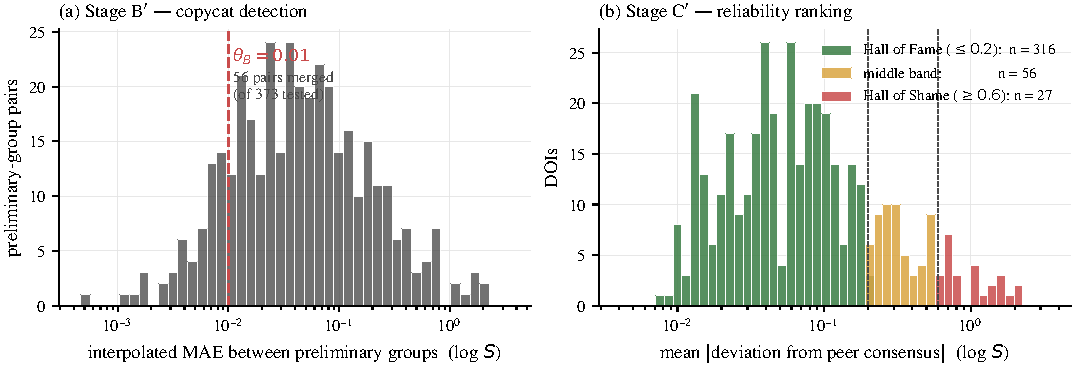
\includegraphics[width=\linewidth]{figures/fig_source_integrity.pdf}
  \caption{\textbf{(a) Stage B$'$ copycat detection.}  Distribution of
    interpolated pair-MAE between preliminary-group pairs sharing at
    least one (solute, solvent) pair.  Dashed line = $\theta_{B'} =
    0.01$ log~S cut.  \textbf{(b) Stage C$'$ reliability ranking.}
    Distribution of per-group mean absolute deviation from peer
    consensus on Apelblat-interpolated curves.  Hall of Fame
    ($\leq 0.2$), middle band, and Hall of Shame ($\geq 0.6$) are
    coloured; dashed vertical lines are the cut-offs.}
  \label{fig:source_integrity}
\end{figure}

\begin{figure}[t]
  \centering
  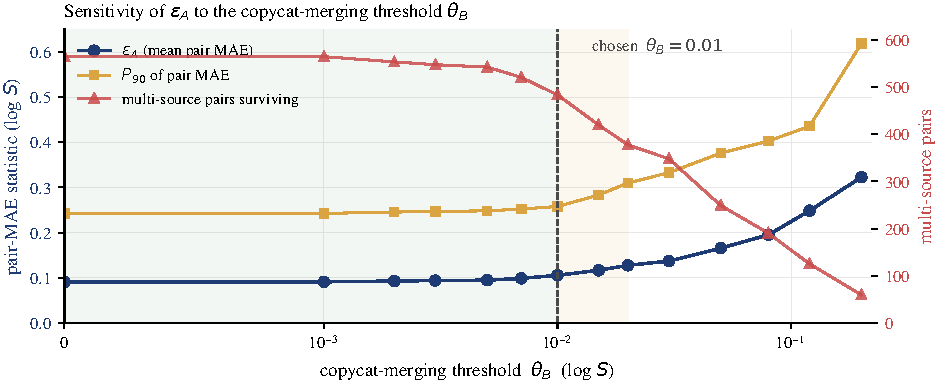
\includegraphics[width=0.9\linewidth]{figures/fig_threshold_sweep.pdf}
  \caption{Sensitivity of $\epsA$ and the multi-source pair count to the
    copycat-merging threshold $\theta_B$.  The chosen value $\theta_B =
    0.01$ (dashed line) sits at the upper edge of the shaded ``safe''
    region, where each merged pair is a genuine copy.  The shaded
    ``cliff'' region $[0.01, 0.02]$ loses $\numval{106}$ multi-source
    pairs --- more than the entire loss incurred between $0$ and
    $0.01$.}
  \label{fig:threshold_sweep}
\end{figure}

\subsection{Thermodynamic curve fits}
\label{sec:apelblat}

To compare laboratories that do not share exact measurement
temperatures, we fit a smooth thermodynamic model to every
$(\mathrm{solute},\mathrm{solvent},\mathrm{group})$ triple with
$\geq 3$ temperature points:

\begin{equation}
  \log_{10} S \;=\; A \;+\; \frac{B}{T} \;+\; C\,\ln T \qquad (\text{Apelblat}),
  \label{eq:apelblat}
\end{equation}

and a reduced form to triples with exactly two temperature points:

\begin{equation}
  \log_{10} S \;=\; A \;+\; \frac{B}{T} \qquad (\text{van't~Hoff}).
  \label{eq:vant}
\end{equation}

Triples with a single temperature point (\numval{507}, $\sim 4.5$\,\%)
cannot be fitted and are excluded from aleatoric interpolation.  Fits
with $R^2 < 0.80$ or RMSE $> 0.30$ log~S (\numval{16}) are flagged as
low-quality and also excluded.  The remaining \numval{11\,063} fits
cover $\geq 95$\,\% of the cleaned data.

Figure~\ref{fig:apelblat}(a) shows the fit-quality distribution: median
$R^2 = 0.9993$, \numval{99.3\,\%} of fits reach $R^2 \geq 0.95$,
\numval{94.9\,\%} reach $R^2 \geq 0.99$.  Thermodynamic monotonicity is
similarly strong: \numval{98.5\,\%} of triples are strictly
monotone-increasing in temperature and only \numval{1} triple shows a
single-step drop exceeding $1$~log~S.
Figure~\ref{fig:apelblat}(b) shows the distribution of per-fit
temperature coverage $\Delta T = T_{\max} - T_{\min}$.  The median
fit spans \numval{30}~K and only a small minority of fits cover less
than the 5~K minimum required for cross-group interpolation
(§\ref{sec:epsA}), confirming that the Apelblat framework supports
aleatoric analysis on the majority of the multi-source pool without
extrapolation.

\begin{figure}[t]
  \centering
  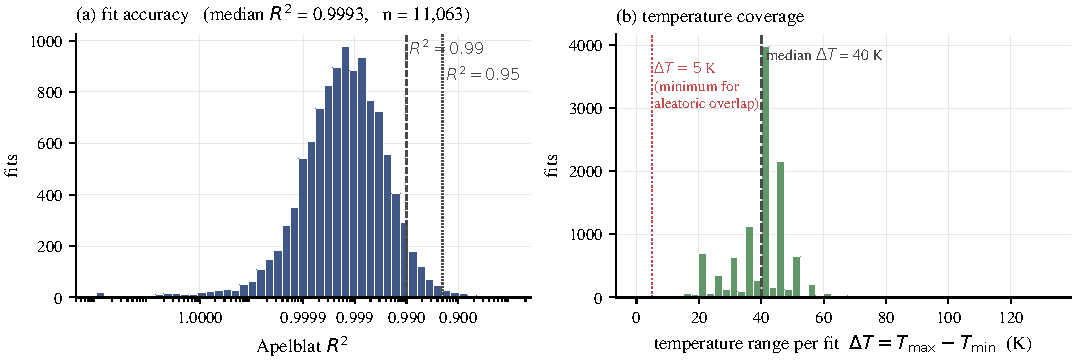
\includegraphics[width=\linewidth]{figures/fig_apelblat_quality.pdf}
  \caption{Apelblat fit quality.  \textbf{(a)}~$R^2$ distribution on a
    reversed log scale ($1 - R^2$ axis).  Most fits have
    $R^2 > 0.99$.  \textbf{(b)}~Temperature coverage $\Delta T$ per
    fit.  Most fits cover more than the 5~K minimum needed for aleatoric
    interpolation; the median fit spans \numval{30}~K.}
  \label{fig:apelblat}
\end{figure}

\subsection{Aleatoric limit}
\label{sec:epsA}

With independence groups and per-group curves established, the
aleatoric limit is a single pair-level statistic on this structure.

\paragraph{Mathematical framework.}
For an $(\mathrm{solute},\mathrm{solvent})$ pair at temperature $T$, the
true solubility $\log_{10} S^{*}(T)$ is unknown.  Independence group $i$
observes $y_i(T) = \log_{10} S^{*}(T) + \varepsilon_i(T)$, where
$\varepsilon_i$ is measurement noise plus any systematic lab effect.
Given fitted curves $f_i(T)$ and $f_j(T)$ for groups $i$ and $j$ on a
reference grid $\mathcal{T}_{ij} = [T^{\min}_{ij}, \ldots, T^{\max}_{ij}]$
at $\Delta T = 1$~K, the interpolated inter-group disagreement at cell
$T$ is

\begin{equation}
  \varepsilon_{ij}(T) \;=\; \bigl|\,f_i(T) - f_j(T)\,\bigr|,
  \label{eq:eps_ij}
\end{equation}

and the \emph{group-pair} MAE is $\mathrm{MAE}_{ij} =
\mathrm{mean}_{T \in \mathcal{T}_{ij}}\,\varepsilon_{ij}(T)$.  Per
(solute, solvent) pair $p$ with independence groups $\mathcal{G}_p$, the
\emph{pair} MAE averages over all within-pair group pairs:

\begin{equation}
  \mathrm{MAE}_p \;=\; \frac{1}{\binom{|\mathcal{G}_p|}{2}}
  \sum_{i<j \in \mathcal{G}_p} \mathrm{MAE}_{ij}.
  \label{eq:mae_pair}
\end{equation}

The aleatoric limit is the \emph{mean} pair MAE across the multi-source
pool $\mathcal{P}$:

\begin{equation}
  \boxed{\;\epsA \;=\; \frac{1}{|\mathcal{P}|}
         \sum_{p \in \mathcal{P}} \mathrm{MAE}_p.\;}
  \label{eq:epsA}
\end{equation}

Two aspects warrant emphasis.  First, $\epsA$ is an \emph{error in
expectation} over pairs and group-pair comparisons, not a summary of
the heavy tail (reported separately below).  Second, we evaluate
\emph{every} cell via the fitted curve (never a measured value) so the
comparison is uniform in character and not biased toward pairs that
happen to share exact measured temperatures.

\paragraph{Primary vs inclusive.}
The Hall-of-Shame groups identified in §\ref{sec:source} consist
overwhelmingly of systematic publication errors (unit swaps, density
errors, silent transcription mistakes) rather than random measurement
noise.  They are excluded from tier consensus labels
(§\ref{sec:tiers}).  For the
aleatoric limit, we report both variants: a \emph{primary} value that
excludes HoS groups (the floor relevant to benchmark performance,
because tier labels use the same pool), and an \emph{inclusive} value
that retains them (useful when comparing against the broader
literature).

\begin{table}[h]
\centering\small
\caption{Primary and inclusive $\epsA$.  95\,\% confidence intervals are
from 5\,000 bootstrap resamples over the multi-source pair pool.}
\label{tab:epsA}
\begin{tabular}{@{}lccccccc@{}}
\toprule
             & $n$ pairs & mean = $\epsA$ & 95\,\% CI       & median & $P_{90}$ & $P_{95}$ & RMSE \\
\midrule
\textbf{Primary} (HoS-excluded)
             & 481       & \textbf{0.106} & [0.093, 0.120] & 0.046  & 0.258    & 0.385    & 0.182 \\
Inclusive    & 511       & 0.158          & [0.132, 0.186] & 0.050  & 0.385    & 0.627    & 0.356 \\
\bottomrule
\end{tabular}
\end{table}

The 95\,\% CI on $\epsA$ (primary) excludes zero by about 7~standard
errors --- the floor is precisely characterised.

\paragraph{Distribution shape.}
Figure~\ref{fig:aleatoric_main} shows the per-pair MAE distribution
together with a gamma fit to the atom-level $|\Delta|$ distribution.
The gamma shape parameter $\alpha = 0.68$ confirms a sub-exponential
(heavy) right tail, which is why the mean (\numval{0.106}) lies well
above the median (\numval{0.046}).  Panel (b) plots the survival
function: 5\,\% of pairs disagree by more than \numval{0.39} log~S, and
the 99\textsuperscript{th}-percentile pair disagrees by more than
$1$~log~S.

\begin{figure}[t]
  \centering
  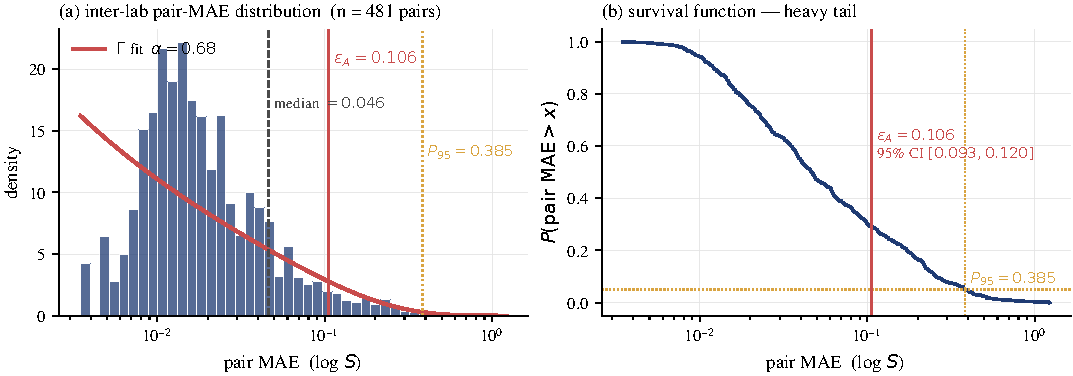
\includegraphics[width=\linewidth]{figures/fig_aleatoric_main.pdf}
  \caption{Primary aleatoric distribution (HoS-excluded).
    \textbf{(a)}~Density of per-pair MAE on log-$x$ axis with a gamma
    fit overlay ($\alpha = 0.68$).  \textbf{(b)}~Survival function
    $P(\mathrm{MAE} > x)$.  Heavy right tail: $P_{95} = 0.39$ log~S.}
  \label{fig:aleatoric_main}
\end{figure}

\paragraph{Per-solvent heterogeneity.}
$\epsA$ is not uniform across solvents (Figure~\ref{fig:per_solvent}).
DMF has the tightest inter-lab agreement at \numval{0.029} log~S across
10 pairs.  Water --- often assumed to be well-characterised because of
the large volume of aqueous data --- has the \emph{highest} mean among
common solvents (\numval{0.110} log~S across \numval{65} pairs), driven
by a thicker tail rather than a higher typical disagreement (its median
is only \numval{0.061}).  This per-solvent heterogeneity motivates the per-solvent evaluation
metric proposed in §\ref{sec:metric_suite} (PS-RMSE): a single global
$\epsA$ under-characterises measurement quality in difficult solvents
and over-characterises it in well-behaved ones.

\begin{figure}[t]
  \centering
  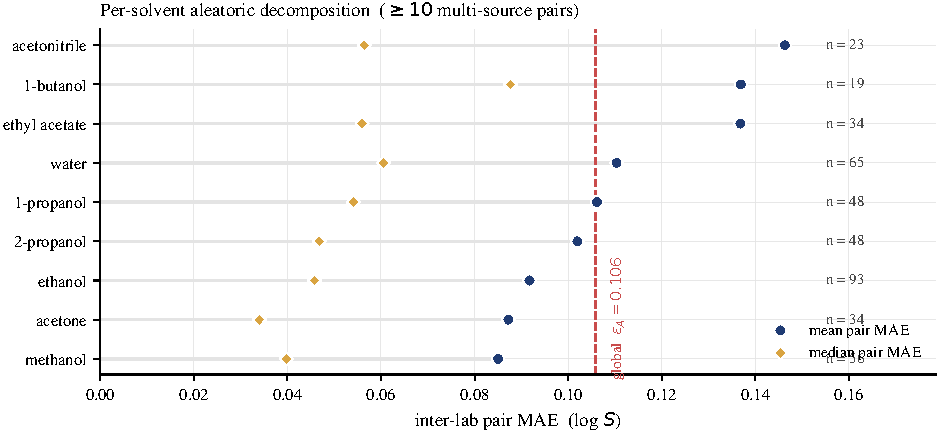
\includegraphics[width=0.95\linewidth]{figures/fig_per_solvent.pdf}
  \caption{Per-solvent aleatoric decomposition (primary, HoS-excluded,
    solvents with $\geq 10$ multi-source pairs).  Lollipops are mean
    pair MAE; diamonds are median; $n$ is the multi-source pair count.
    Dashed vertical line is the global $\epsA = 0.106$.}
  \label{fig:per_solvent}
\end{figure}

\paragraph{Reconciliation with Palmer \& Mitchell (2014).}
The \numval{0.6--0.8} log~S figure cited in the aqueous-solubility
literature is not wrong --- it is simply a different summary statistic
on the same underlying distribution.  Figure~\ref{fig:palmer} overlays
our full inclusive atom-level $|\Delta|$ distribution with the Palmer
band (shaded).  Their number coincides with \emph{our} $P_{90}$--$P_{95}$
at \numval{0.39}--\numval{0.63} log~S and with our RMSE (\numval{0.36}),
but not with the mean (\numval{0.16}) or median (\numval{0.05}).  A
practitioner who quotes the \emph{expected} inter-lab error --- the
number models compete against in expectation --- should quote
$\epsA \approx \numval{0.11}$ log~S; a practitioner who quotes the
95\textsuperscript{th}-percentile worst case --- the noise a model
faces on its hardest test point --- can legitimately still quote
\numval{0.6}.

\begin{figure}[t]
  \centering
  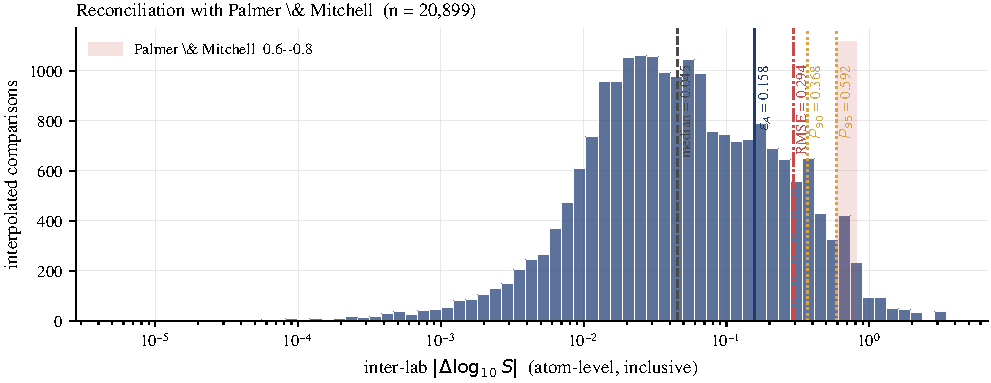
\includegraphics[width=0.9\linewidth]{figures/fig_palmer.pdf}
  \caption{Reconciliation with \citet{palmer2014dataquality}.  The
    inclusive atom-level $|\Delta \log_{10} S|$ distribution
    ($n = 20\,899$ interpolated comparisons) is plotted on a log-$x$
    axis; vertical lines are our summary statistics.  The shaded band
    is Palmer \& Mitchell's quoted 0.6--0.8 log~S aqueous range, which
    coincides with our $P_{90}$--$P_{95}$ and RMSE, not with the
    expected error.}
  \label{fig:palmer}
\end{figure}

\paragraph{Cross-database validation.}
Our $\epsA$ characterises consistency \emph{within} \textsc{BigSolDB}
after copycat correction and Hall-of-Shame exclusion.  A natural
question is whether this floor extends across databases compiled from
different source selections and unit conventions.

\todo{Cross-database validation not yet computed.  Plan: match aqueous
compounds common to \textsc{BigSolDB} and \textsc{AqSolDB}
\citep{sorkun2019aqsoldb} under our Option-D canonicalization, report
matched-set size, RMSE, MAE and systematic bias, and compare to the
intra-\textsc{BigSolDB}{} $\epsA$ reported above.  Expect the
cross-database disagreement to be substantially larger than $\epsA$
owing to differences in unit convention, source selection and
temperature handling across the two databases.}

Independently of the exact cross-database number, the intra-database
floor reported above is the ceiling relevant to our \scthree{}
benchmark, because \scthree{} is constructed entirely from
\textsc{BigSolDB}.

\section{Benchmark design}
\label{sec:benchmark}

With a cleaned dataset (§\ref{sec:data_curation}) and a calibrated
noise floor (§\ref{sec:aleatoric}), we can now build the benchmark
itself.  \scthree{} is designed to answer three distinct generalisation
questions simultaneously: can a model predict (i) a new
$(\mathrm{solute}, \mathrm{solvent})$ pair in a familiar solvent,
(ii) the same solute in a solvent it has never seen, and
(iii) a new solute against consensus-calibrated labels with per-point
uncertainty $\sigma$?  Each question corresponds to a separate
evaluation set.  The construction is: a \emph{tier-test pool} with
consensus labels from multi-source agreement, and a \emph{training
pool} drawn from the complement that is further split by
solvent-frequency into in-distribution (Train, Eval) and
out-of-distribution (OOD) sets.

\subsection{Tier construction}
\label{sec:tiers}

The tiers are the benchmark's evaluation with calibrated ground truth
and $\sigma$.  They are built from the \numval{481} multi-source pairs
that survive
(i) the copycat merging of §\ref{sec:source}, (ii) the Hall-of-Shame
exclusion, and (iii) the fit-quality gate of §\ref{sec:apelblat}.  For
each eligible pair we compute the pair MAE (equation~\ref{eq:mae_pair})
and assign it to every tier whose MAE threshold it satisfies:

\begin{center}
\renewcommand{\arraystretch}{1.08}\small
\begin{tabular}{@{}lll@{}}
\toprule
Tier   & Pair MAE threshold          & Meaning \\
\midrule
\textbf{Gold}   & $\leq 0.1$ log S    & consensus labels disagree by at most $\sim\epsA$ \\
\textbf{Silver} & $\leq 0.2$ log S    & within a factor of $\sim 2\epsA$ \\
\textbf{Bronze} & $\leq 0.5$ log S    & within a factor of $\sim 5\epsA$ \\
\bottomrule
\end{tabular}
\end{center}

The tiers are \emph{nested}: $\text{Gold} \subset \text{Silver} \subset
\text{Bronze}$.  The naming is designed so that a \textbf{tighter tier
label corresponds to a better-characterised ground truth}, not to a
harder modelling task.  A model evaluated on Gold is being compared
against the tightest available reference labels; Bronze is a broader
net that keeps more pairs at the cost of looser consensus.

\paragraph{Consensus labels.}
For each $(\mathrm{solute}, \mathrm{solvent}, T)$ triple in a tier pair,
we evaluate every contributing independence group's Apelblat /
van't-Hoff fit at $T$ and define the consensus label as the mean of
those evaluations, excluding Hall-of-Shame groups.  The per-point
uncertainty $\sigma$ is the standard deviation across the same set of
evaluations.  When fewer than two groups contribute at a given $T$,
$\sigma$ is undefined and the row carries a hard label with no
uncertainty; this happens on \numval{14.4}\,\% of tier rows overall.

\paragraph{Uncertainty floor.}
A standard deviation from two nearly-identical fits can underestimate
true measurement spread.  We therefore floor $\sigma$ at $0.012$ log S
($\approx \epsA / 10$) --- the median Apelblat fit RMSE
(§\ref{sec:apelblat}) --- to prevent a handful of suspiciously-tight
$\sigma$s from dominating $Z$-normalised losses.

\paragraph{Tier statistics.}
Table~\ref{tab:tiers} shows size and $\sigma$ distribution per tier.
Median $\sigma$ ranges from \numval{0.019} (Gold) through \numval{0.024}
(Silver) to \numval{0.031} (Bronze); the Gold tail is much shorter
($P_{95} = \numval{0.078}$ vs Bronze $P_{95} = \numval{0.245}$),
reflecting the tighter pair-MAE cap.  Figure~\ref{fig:tier_sigma} shows
the full $\sigma$ distribution per tier: the Gold distribution is
entirely below Bronze's tail.

\begin{table}[h]
\centering\small
\caption{SC$^{3}$ tier composition and $\sigma$ statistics.  Nested:
Gold $\subset$ Silver $\subset$ Bronze.  $\sigma$-coverage is the
fraction of tier rows with a defined per-point uncertainty; remaining
rows have a hard label only.}
\label{tab:tiers}
\begin{tabular}{@{}lrrrr cccc@{}}
\toprule
Tier   & rows  & pairs & solutes & solvents
       & $\sigma$-cov. & median $\sigma$ & mean $\sigma$ & $P_{95}\ \sigma$ \\
\midrule
Gold   & 4\,507 & 335 & 129 & 26 & 76.5\%  & 0.019 & 0.028 & 0.078 \\
Silver & 5\,475 & 400 & 141 & 27 & 76.9\%  & 0.024 & 0.042 & 0.130 \\
Bronze & 6\,331 & 469 & 148 & 30 & 77.1\%  & 0.031 & 0.066 & 0.245 \\
\bottomrule
\end{tabular}
\end{table}

\begin{figure}[t]
\centering
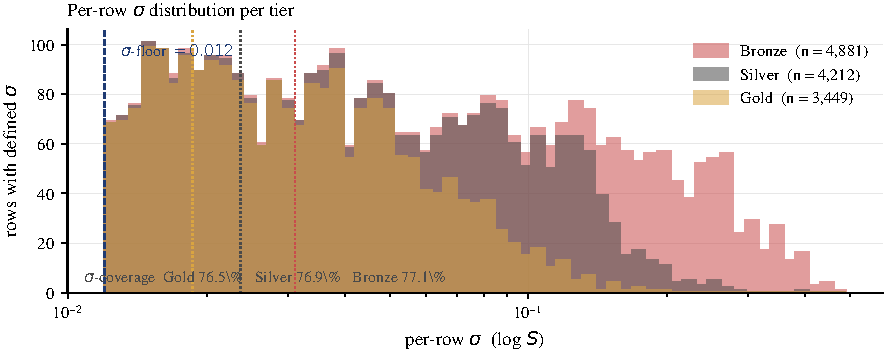
\includegraphics[width=0.9\linewidth]{figures/fig_tier_sigma.pdf}
\caption{Per-row $\sigma$ distribution in the three nested tiers, log-$\sigma$
 axis.  Dashed vertical line at the $\sigma$-floor $= 0.012$ log S; dotted
 lines mark per-tier medians.  Gold's distribution is concentrated between
 the floor and $\sim 0.03$ log S; Bronze has a much longer tail out to
 $\sigma > 0.2$ log S.  $\sigma$-coverage is near-identical across tiers
 ($\sim 77\,\%$), so the tail difference is about \emph{quality} of
 uncertainty, not quantity.}
\label{fig:tier_sigma}
\end{figure}

\subsection{Training, evaluation, and OOD splits}
\label{sec:splits}

Tiers consume only a thin slice of the cleaned pool; the complement
forms the training and in-distribution test sets, and the long-tail
solvents become the out-of-distribution test set.  The
\numval{148} solutes that appear in any tier are fully excluded from
the training pool at the $(\mathrm{solute}, \mathrm{solvent}, T)$
level --- no row containing such a solute survives into Train, Eval,
or OOD.
The remaining \numval{80\,312} rows are split by solvent frequency:

\begin{itemize}[leftmargin=1.25em,itemsep=1pt]
\item \textbf{Top-25 solvents} (ranked by training-pool row count,
covering \numval{85.1\,\%} of the training pool) form the
\emph{in-distribution} region.  Within this region, \numval{10\,\%} of
each solvent's solute list is held out as \textbf{Eval}; the remainder
is \textbf{Train}.
\item \textbf{Remaining \numval{181} solvents} form the \textbf{OOD}
set.  By construction a model will never have been trained on any of
these solvents, which tests whether it can generalise across the
solvent axis.
\end{itemize}

Table~\ref{tab:splits} summarises the final composition.

\begin{table}[t]
\centering\small
\caption{SC$^{3}$ splits and tiers.  All six evaluation subsets have
zero solute overlap with training (see Table~\ref{tab:antileakage}).
Solvent overlap with Train is intentional for Eval (in-distribution)
and tiers (calibrated labels); OOD has zero solvent overlap with Train
by construction.}
\label{tab:splits}
\begin{tabular}{@{}llrrrr@{}}
\toprule
& Role                           & rows     & solutes & solvents & (solute, solvent) pairs \\
\midrule
\multicolumn{6}{l}{\textit{Training pool (\numval{80\,312} rows after tier exclusion)}} \\
Train  & training set                   & 61\,403  & 1\,144  & 25       & 6\,840 \\
Eval   & new-pair, in-distribution      &  6\,969  &    534  & 25       &    771 \\
OOD    & new-solvent (151 unseen)       & 11\,940  &    586  & 161      &  1\,450 \\
\midrule
\multicolumn{6}{l}{\textit{Tier test pool (solutes fully absent from training pool)}} \\
Gold   & tight consensus, $\sigma$-cal.  &  4\,507  &    129  &  26      &    335 \\
Silver & looser consensus, $\sigma$-cal. &  5\,475  &    141  &  27      &    400 \\
Bronze & broadest, $\sigma$-cal.         &  6\,331  &    148  &  30      &    469 \\
\bottomrule
\end{tabular}
\end{table}

\paragraph{Generalisation axes exposed.}
The three evaluation sets test distinct notions of generalisation:

\begin{itemize}[leftmargin=1.25em,itemsep=1pt]
  \item \textbf{Eval} tests \emph{new (solute, solvent) pairs} in
    already-seen solvents.  A model must interpolate across the
    solute axis.
  \item \textbf{OOD} tests \emph{new solvents} (the \numval{161}
    long-tail solvents).  Solute may have been seen in a different
    solvent, but the target solvent is unseen.  Some solvents have few
    measurements; we therefore report OOD metrics with the per-solvent
    split-out explicitly (§\ref{sec:metrics}).
  \item \textbf{Gold / Silver / Bronze} test \emph{new solutes} against
    calibrated consensus labels with $\sigma$.  Any of the 148 tier
    solutes has been removed from Train/Eval/OOD, so all tier tests
    are solute-level out-of-distribution.
\end{itemize}

\paragraph{Anti-leakage verification.}
Every overlap that must be zero, is zero (Table~\ref{tab:antileakage}).
Solute overlap between Train and Eval is expected to be positive
($\numval{520}$ solutes) because Eval is a held-out slice of the
in-distribution solute--solvent grid; pair-level overlap between Train
and Eval remains zero by construction of the hold-out.

\begin{table}[h]
\centering\small
\caption{Anti-leakage verification.  Every cell reports the count of
(solute, solvent) pair overlaps between two splits.  Zero everywhere
except the two off-diagonal entries that are expected to share solutes
but never pairs (shaded).  All checks pass.}
\label{tab:antileakage}
\begin{tabular}{@{}lcccccc@{}}
\toprule
          & Train & Eval & OOD & Gold & Silver & Bronze \\
\midrule
Train     & ---   & 0    & 0   & 0    & 0      & 0      \\
Eval      & 0     & ---  & 0   & 0    & 0      & 0      \\
OOD       & 0     & 0    & --- & 0    & 0      & 0      \\
Gold      & 0     & 0    & 0   & ---  & nested & nested \\
Silver    & 0     & 0    & 0   & nested & ---  & nested \\
Bronze    & 0     & 0    & 0   & nested & nested & ---   \\
\bottomrule
\end{tabular}
\end{table}

\begin{figure}[h]
\centering
\figplaceholder{fig_splits_diagram.pdf}{0.30}{%
  Two-axis schematic of the leakage-hard splits.  Horizontal axis = solvent
  set (25 ID solvents on the left, 161 OOD solvents on the right);
  vertical axis = solute set (training-pool solutes vs.\ tier solutes,
  fully disjoint).  Train (top-left), Eval (top-left held-out pairs),
  OOD (top-right, ID solutes in unseen solvents), and tiers
  (bottom-left, tier solutes in ID solvents with calibrated
  $\sigma$).  Cell row counts: Train $61\,403$, Eval $6969$,
  OOD $11\,940$, Bronze $6331$.  Use coloured rectangles with row counts
  inside and a legend identifying each split.%
}
\caption{Three generalisation axes the splits expose.  \emph{Eval}
tests new (solute, solvent) pairs in familiar solvents;
\emph{OOD} tests unseen solvents; the tiers test new solutes in
familiar solvents \emph{with calibrated $\sigma$}.}
\label{fig:splits_diagram}
\end{figure}

\section{Metrics}
\label{sec:metrics}

With the splits in place (§\ref{sec:benchmark}), we turn to scoring.
Reporting aggregate RMSE works for single-solvent regression but fails
here for four distinct reasons rooted in the multi-solvent structure
of the data.  We characterise those reasons empirically on \scthree{},
then define the five-metric suite we recommend reporting for every
model.

\subsection{Why multi-solvent is different}
\label{sec:multimodal}

\paragraph{Per-solvent location shift.}
Across the \numval{206} cleaned solvents, per-solvent log~S means span
\textbf{\numval{7.98} log units} (minimum \numval{-6.93}, maximum
\numval{+1.05}) --- nine orders of magnitude in equivalent
concentration.  Figure~\ref{fig:solvent_dist} shows the per-solvent
log~S distribution for the top-20 solvents by row count, ordered by
their per-solvent mean.  The densities overlap substantially in the
middle of the range (both water and alcohols contain solutes spanning
most of the dataset's log~S range) but their locations differ by up
to seven log units.

\begin{figure}[t]
\centering
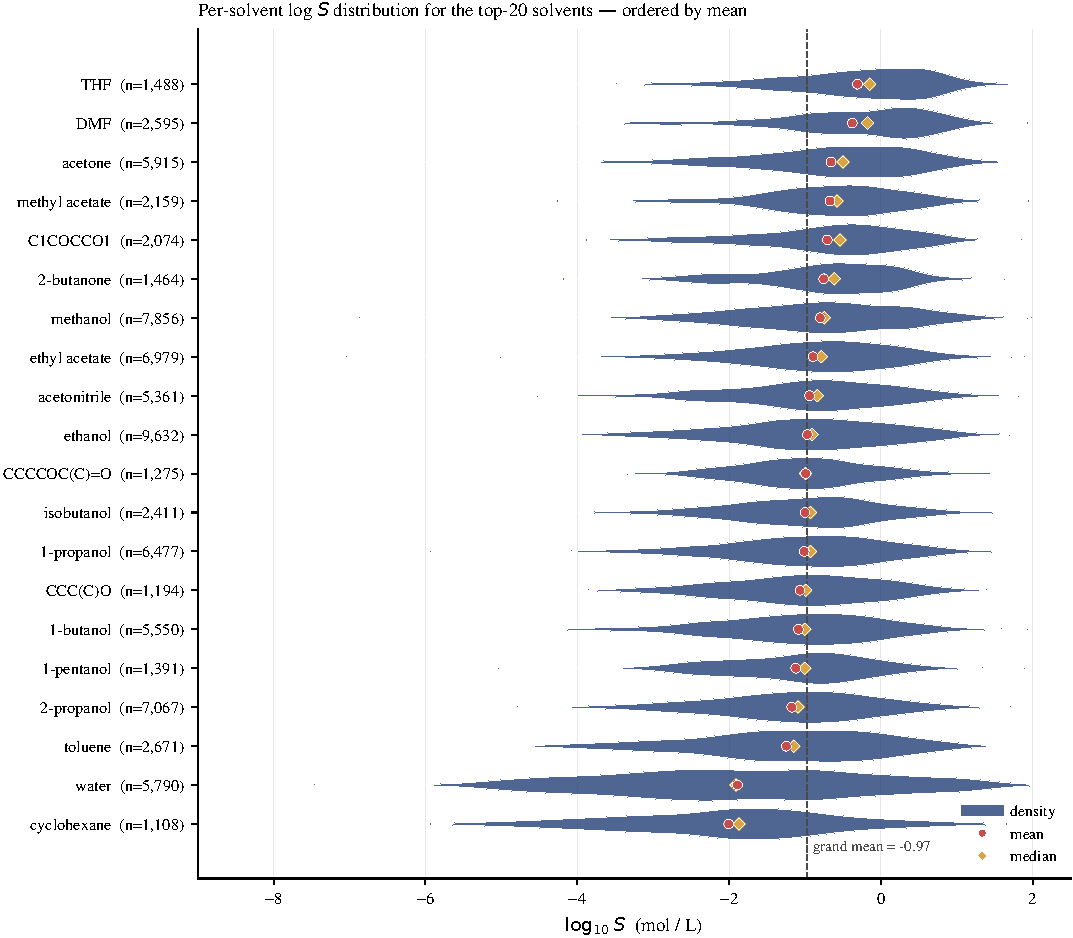
\includegraphics[width=\linewidth]{figures/fig_solvent_distributions.pdf}
\caption{Per-solvent log~$S$ distribution (violin) for the top-20
  solvents by row count, ordered by per-solvent mean.  Red marker =
  mean, gold diamond = median, dashed line = grand mean.  The top-to-
  bottom mean span is $\sim 7$ log~$S$; \emph{any} predictor that
  correctly identifies the solvent absorbs most of that variance for
  free.}
\label{fig:solvent_dist}
\end{figure}

\paragraph{Variance decomposition.}
A one-way ANOVA of cleaned log~S on solvent identity attributes
\textbf{\numval{11.7\,\%}} of total variance to the between-solvent
location shift ($F = \numval{69.9}$ across \numval{206} solvents,
$p < 10^{-300}$).  On OOD, which is built from the long-tail solvents,
the between-solvent fraction rises to \textbf{\numval{22.1\,\%}}
because the long-tail solvents include extremes (e.g.,
1,1-dichloroethane with mean log~S $= -6.93$).  Within each tier the
fraction is closer to \numval{9.3}--\numval{9.9\,\%}.

\paragraph{Dummy-baseline R$^2$.}
We quantify how much of this variance is ``free'' for a trivial model.
A predictor that returns the \emph{per-solvent training mean} (no
solute information, no temperature) achieves the R$^2$ values in
Figure~\ref{fig:dummy_baseline}.  On the in-distribution Eval split,
the baseline scores $R^2 = \numval{+0.053}$ --- positive, non-trivial,
and achievable by a model that only memorises the 25 training-solvent
means.  On the three tiers it scores $R^2 \in [-0.003, +0.017]$, near
zero but within the ID solvent space.  On OOD, where \numval{161} of
\numval{161} test solvents are never seen during training and the
baseline necessarily falls back to the grand training mean, it
\textbf{goes negative} ($R^2 = \numval{-0.062}$) --- the grand mean
is actively worse than no prediction at all on the long-tail solvents.

\begin{figure}[t]
\centering
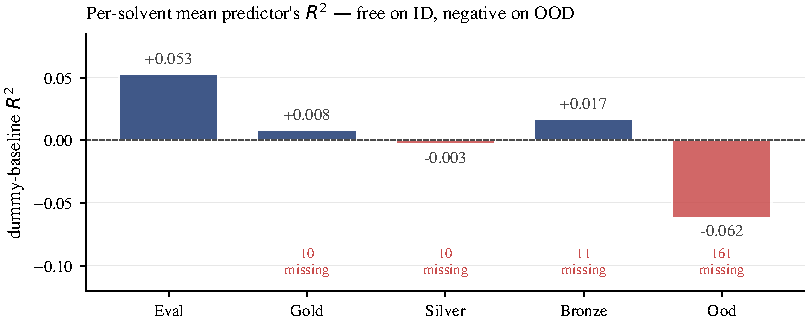
\includegraphics[width=0.75\linewidth]{figures/fig_dummy_baseline.pdf}
\caption{Per-solvent-mean predictor's $R^2$ across the five evaluation
splits.  Positive on in-distribution Eval, near-zero on tiers, and
\emph{negative} on OOD (\numval{161} solvents unseen during training,
so the predictor falls back to the grand mean).  Motivates a metric
suite in which aggregate $R^2$ or RMSE does not reward solvent
identification.}
\label{fig:dummy_baseline}
\end{figure}

\paragraph{Count domination.}
The top-5 solvents (\emph{ethanol, methanol, 2-propanol, ethyl
acetate, 1-propanol}) account for \textbf{\numval{37.5\,\%}} of the
cleaned rows and \textbf{\numval{44.2\,\%}} of Train; the top-25
account for \numval{84.5\,\%} and cover 100\,\% of Train / Eval by
construction.  An aggregate-row metric such as RMSE is therefore,
functionally, a metric on those five solvents.  Reporting only
aggregates would hide per-solvent regression on the long-tail set.

\paragraph{MAPE is broken here.}
\numval{5.6\,\%} of cleaned rows have $|\logS| < 0.1$, and
\numval{28.5\,\%} have $|\logS| < 0.5$ --- the MAPE denominator is
small or zero for a material fraction of the data.  MAPE is therefore
unbounded for any model that makes ordinary-magnitude absolute errors
on these rows and should not be reported as a headline statistic.

\paragraph{Heavy-tailed labels.}
The $|y - \bar{y}|$ distribution has mean/median ratio
$\numval{1.19}$ ($P_{95} = \numval{2.27}$, $P_{99} =
\numval{3.43}$).  RMSE is tail-sensitive in a regime this heavy,
motivating a median absolute error as a robust complement.

\subsection{The SC$^3$ metric suite}
\label{sec:metric_suite}

Combining the above, we define five primary metrics, with
\textbf{PS-RMSE} as the single headline.  Definitions are in
Table~\ref{tab:metrics}.

\begin{table}[h]
\centering\small
\caption{SC$^{3}$ metric suite.  $n$ = rows in the split; $|\mathcal{S}|$
= solvents in the split; $\sigma_i$ = per-row calibrated uncertainty
(tiers only).  The ``applicability'' column lists the splits on which
each metric is computed.  MAPE is reported for diagnostic purposes only.}
\label{tab:metrics}
\begin{tabular}{@{}llcl@{}}
\toprule
Metric         & Formula & Applicability       & Role \\
\midrule
RMSE           & $\sqrt{\frac{1}{n}\sum_i (\hat y_i - y_i)^2}$
               & all
               & count-weighted; baseline \\[1pt]
MAE            & $\frac{1}{n}\sum_i |\hat y_i - y_i|$
               & all
               & less tail-sensitive than RMSE \\[1pt]
MedAE          & $\mathrm{median}_i\,|\hat y_i - y_i|$
               & all
               & robust on heavy-tailed residuals \\[1pt]
\textbf{PS-RMSE} & $\frac{1}{|\mathcal{S}|}\sum_{s\in\mathcal{S}}
                   \mathrm{RMSE}_s$
               & all
               & \textbf{strips count and between-solvent inflation} \\[1pt]
Z-RMSE         & $\sqrt{\frac{1}{n_\sigma}\sum_{i:\sigma_i\ \text{def.}}
                       \bigl((\hat y_i - y_i)/\sigma_i\bigr)^2}$
               & Gold, Silver, Bronze
               & error in units of the aleatoric floor \\[1pt]
\textit{MAPE}  & $\frac{1}{n}\sum_i |\hat y_i - y_i|/|y_i|$
               & \textit{diagnostic}
               & diverges for $|\logS| < \varepsilon$ \\
\bottomrule
\end{tabular}
\end{table}

\paragraph{PS-RMSE.}  Per-solvent RMSE averaged equally across
solvents.  This resolves both the variance-decomposition and
count-domination problems from §\ref{sec:multimodal} in one stroke:
between-solvent location shifts cancel out of the per-solvent RMSE,
and each solvent contributes equally regardless of its row count.
For $|\mathcal{S}|$ large enough, PS-RMSE approaches the
``within-solvent'' RMSE that the ANOVA identifies as the honest
prediction-error variance.

\paragraph{Z-RMSE.}  Error in units of the aleatoric floor.  On rows
where $\sigma_i$ is defined (median \numval{77}\,\% of tier rows,
Table~\ref{tab:tiers}), Z-RMSE $= 1$ means a model is operating at
the measurement-noise limit; Z-RMSE $= 10$ means errors are an order
of magnitude larger than irreducible label uncertainty.  Because
\scthree{} calibrates $\sigma$ per point, Z-RMSE is a
\emph{per-measurement} comparison to the floor, not a comparison to
a single global $\epsA$.

\paragraph{Computational domains.}
Not every metric is computable on every split: Z-RMSE requires
per-row $\sigma$ and is therefore only defined on Gold / Silver /
Bronze, and even there on roughly \numval{77\,\%} of rows.
Table~\ref{tab:metric_domain} reports the effective sample size per
metric per split.

\begin{table}[h]
\centering\small
\caption{Effective sample size per metric per split.  RMSE, MAE, MedAE,
and per-solvent RMSE (PS-RMSE) are computable on every row and every
solvent present in the split.  Z-RMSE is defined only on tier rows
with multi-group consensus ($\sigma$ defined); columns $n_{\sigma}$ and
``Z-coverage'' report the count and fraction accordingly.}
\label{tab:metric_domain}
\begin{tabular}{@{}lrrrrrrr@{}}
\toprule
Split  & rows   & solvents & $n_{\mathrm{RMSE/MAE/MedAE}}$ & $|\mathcal{S}|$ (PS-RMSE) &
         $n_{\sigma}$ & Z-coverage \\
\midrule
Train  & 61\,403 &  25 & 61\,403 &  25 & ---   & ---    \\
Eval   &  6\,969 &  25 &  6\,969 &  25 & ---   & ---    \\
OOD    & 11\,940 & 161 & 11\,940 & 161 & ---   & ---    \\
Gold   &  4\,507 &  26 &  4\,507 &  26 & 3\,449 & 76.5\% \\
Silver &  5\,475 &  27 &  5\,475 &  27 & 4\,212 & 76.9\% \\
Bronze &  6\,331 &  30 &  6\,331 &  30 & 4\,881 & 77.1\% \\
\bottomrule
\end{tabular}
\end{table}


% =============================================================================
\section{Baselines}
\label{sec:baselines}

\todo{One short paragraph: $\sim 27$ baselines across seven families,
all consuming the same $(\text{solute}, \text{solvent}, T)$ input,
matched seeds, no per-method HP-tuning advantage in the headline
table.  Full hyperparameters in Appendix~\ref{app:hparams}.}

\begin{itemize}[leftmargin=*]
  \item \textbf{Thermodynamic / group contribution} -- ESOL, GSE,
        UNIFAC, Abraham LFER.
  \item \textbf{Descriptor + GBDT} -- LightGBM, CatBoost, XGBoost,
        Random Forest on RDKit + temperature features.  Includes
        Abraham-ML and UNIFAC-ML variants.
  \item \textbf{Fingerprint + ML} -- same trees on Morgan ECFP4; GP
        with Tanimoto kernel.
  \item \textbf{Learned descriptors} -- FastProp, FastSolv, Dissolvr,
        MLP on RDKit.
  \item \textbf{Graph neural networks} -- GCN, GAT, GIN, SolubNet,
        Chemprop D-MPNN, MolMerger.
  \item \textbf{Sequence model} -- SolTranNet.
  \item \textbf{Foundation model} -- Uni-Mol2 (frozen and fine-tuned).
\end{itemize}

\todo{Optional: drop in Figure~\ref{fig:family_tree} schematic if we
keep it; otherwise remove and let Table~\ref{tab:main_results} carry
the family grouping.}

\begin{figure}[h]
\centering
\figplaceholder{fig_family_tree.pdf}{0.30}{%
  Compact taxonomy of the $\sim 27$ baselines, grouped by the seven
  families above.  Decorate each leaf with input type
  (\SMILES{} / descriptor / graph) and parameter count where
  applicable.%
}
\caption{Baseline taxonomy.}
\label{fig:family_tree}
\end{figure}

% =============================================================================
\section{Main results}
\label{sec:results}

Table~\ref{tab:main_results} reports mean$\pm$std metrics across five random seeds on Eval, OOD, and the three consensus tiers.
\textsc{LightGBM} with RDKit descriptors currently achieves the strongest headline PS-RMSE on Bronze among completed runs; graph baselines and several foundation-model rows remain pending reruns or hyperparameter passes---cells marked ``---'' should be interpreted as \emph{not yet reported}, not as missing experiments.
Once all entries are populated, this section will summarise (i)~which modelling family dominates PS-RMSE and Z-RMSE at fixed compute, (ii)~descriptor vs.\ fingerprint vs.\ graph contrasts at matched inputs where possible, and (iii)~how far the best models sit above the aleatoric references of §\ref{sec:aleatoric} and §\ref{sec:data_scaling}.

% Main benchmark results table.  Format ported from the v1 paper
% (sc3-benchmark/paper/tables/main_results.tex).  All numerical entries
% are dashed pending the v2 + HP-tuned rerun on Gold/Silver/Bronze; only
% the row structure is fixed.

\definecolor{first}{HTML}{C6EFCE}
\definecolor{second}{HTML}{DAEFC6}
\definecolor{third}{HTML}{EEF5DD}

\providecommand{\fst}[1]{\cellcolor{first}\textbf{#1}}
\providecommand{\snd}[1]{\cellcolor{second}#1}
\providecommand{\trd}[1]{\cellcolor{third}#1}

\begin{table*}[t]
  \caption{\scthree{} benchmark.  Mean{\scriptsize$\pm$std} over 5 seeds;
  PS-RMSE is the primary metric (top 3 per column highlighted).
  Time is per-seed on single CPU thread or A100 GPU.
  Cells remain dashed where reruns are not yet available.}
  \label{tab:main_results}
  \centering
  \footnotesize
  \setlength{\tabcolsep}{3pt}
  \begin{tabular}{@{}l l cc c ccc c r@{}}
    \toprule
    & & \multicolumn{2}{c}{Eval} & OOD & \multicolumn{3}{c}{PS-RMSE $\downarrow$} & Z$\downarrow$ & Time \\
    \cmidrule(lr){3-4} \cmidrule(lr){6-8}
    Method & Repr. & RMSE & $R^2$ & RMSE & Gold & Silver & Bronze & Bronze & (s) \\
    \midrule
    \multicolumn{10}{@{}l}{\textit{Descriptor + tree ensembles}} \\[2pt]
    LightGBM      & RDKit   & 0.493 $\pm$ 0.003 & 0.816 $\pm$ 0.003 & 0.611 $\pm$ 0.004 & 0.604 $\pm$ 0.008 & 0.561 $\pm$ 0.009 & 0.561 $\pm$ 0.010 & 35.280 $\pm$ 0.308 & --- \\
    Abraham ML    & RDKit   & --- & --- & --- & --- & --- & --- & --- & --- \\
    CatBoost      & RDKit   & 0.477 $\pm$ 0.008 & 0.827 $\pm$ 0.006 & 0.611 $\pm$ 0.005 & 0.635 $\pm$ 0.029 & 0.597 $\pm$ 0.028 & 0.593 $\pm$ 0.032 & 36.070 $\pm$ 0.535 & --- \\
    Dissolvr      & Domain  & 0.490 $\pm$ 0.004 & 0.818 $\pm$ 0.003 & 0.619 $\pm$ 0.003 & 0.623 $\pm$ 0.009 & 0.578 $\pm$ 0.004 & 0.576 $\pm$ 0.005 & 36.054 $\pm$ 0.501 & --- \\
    XGBoost       & RDKit   & 0.494 $\pm$ 0.010 & 0.815 $\pm$ 0.007 & 0.641 $\pm$ 0.013 & 0.651 $\pm$ 0.015 & 0.614 $\pm$ 0.014 & 0.604 $\pm$ 0.016 & 36.601 $\pm$ 0.984 & --- \\
    Random Forest & RDKit   & 0.517 $\pm$ 0.001 & 0.797 $\pm$ 0.001 & 0.624 $\pm$ 0.001 & 0.683 $\pm$ 0.004 & 0.629 $\pm$ 0.002 & 0.634 $\pm$ 0.002 & 36.721 $\pm$ 0.125 & --- \\
    Tayyebi       & Mordred & 0.573 $\pm$ 0.001 & 0.752 $\pm$ 0.001 & 0.717 $\pm$ 0.001 & 0.795 $\pm$ 0.009 & 0.728 $\pm$ 0.006 & 0.738 $\pm$ 0.005 & 40.337 $\pm$ 0.228 & --- \\
    \midrule
    \multicolumn{10}{@{}l}{\textit{Fingerprint-based}} \\[2pt]
    CatBoost      & Morgan   & 0.546 $\pm$ 0.002 & 0.774 $\pm$ 0.002 & 0.728 $\pm$ 0.008 & 0.878 $\pm$ 0.018 & 0.819 $\pm$ 0.017 & 0.766 $\pm$ 0.021 & 42.782 $\pm$ 0.596 & --- \\
    XGBoost       & Morgan   & 0.565 $\pm$ 0.004 & 0.758 $\pm$ 0.003 & 0.778 $\pm$ 0.002 & 0.985 $\pm$ 0.018 & 0.918 $\pm$ 0.012 & 0.829 $\pm$ 0.014 & 47.372 $\pm$ 0.578 & --- \\
    Random Forest & Morgan   & 0.578 $\pm$ 0.001 & 0.747 $\pm$ 0.001 & 0.756 $\pm$ 0.001 & 0.817 $\pm$ 0.003 & 0.782 $\pm$ 0.004 & 0.719 $\pm$ 0.004 & 44.722 $\pm$ 0.032 & --- \\
    LightGBM      & Morgan   & 0.532 $\pm$ 0.004 & 0.785 $\pm$ 0.003 & 0.778 $\pm$ 0.006 & 0.924 $\pm$ 0.013 & 0.862 $\pm$ 0.010 & 0.792 $\pm$ 0.011 & 45.271 $\pm$ 0.384 & --- \\
    GP            & Tanimoto & 0.627 $\pm$ 0.013 & 0.702 $\pm$ 0.012 & 0.958 $\pm$ 0.012 & 1.038 $\pm$ 0.054 & 0.967 $\pm$ 0.040 & 0.909 $\pm$ 0.028 & 50.170 $\pm$ 1.524 & --- \\
    \midrule
    \multicolumn{10}{@{}l}{\textit{Deep learning (descriptors)}} \\[2pt]
    FastProp & RDKit & 0.465 $\pm$ 0.006 & 0.837 $\pm$ 0.004 & 0.675 $\pm$ 0.013 & 0.768 $\pm$ 0.041 & 0.732 $\pm$ 0.034 & 0.689 $\pm$ 0.031 & 38.609 $\pm$ 1.474 & --- \\
    FastSolv & RDKit & 0.471 $\pm$ 0.006 & 0.832 $\pm$ 0.004 & 0.708 $\pm$ 0.008 & 0.791 $\pm$ 0.063 & 0.748 $\pm$ 0.045 & 0.693 $\pm$ 0.039 & 38.282 $\pm$ 0.927 & --- \\
    MLP      & RDKit & 0.470 $\pm$ 0.004 & 0.833 $\pm$ 0.003 & 0.720 $\pm$ 0.007 & 0.813 $\pm$ 0.030 & 0.768 $\pm$ 0.034 & 0.708 $\pm$ 0.036 & 39.999 $\pm$ 1.087 & --- \\
    \midrule
    \multicolumn{10}{@{}l}{\textit{Graph neural networks}} \\[2pt]
    Chemprop    & D-MPNN   & --- & --- & --- & --- & --- & --- & --- & --- \\
    Solvaformer & SE(3)    & --- & --- & --- & --- & --- & --- & --- & --- \\
    GCN         & Dual enc & 0.599 $\pm$ 0.016 & 0.728 $\pm$ 0.015 & 0.776 $\pm$ 0.031 & 1.066 $\pm$ 0.039 & 1.014 $\pm$ 0.049 & 0.979 $\pm$ 0.042 & 55.155 $\pm$ 2.883 & --- \\
    SolubNet    & TAGConv  & --- & --- & --- & --- & --- & --- & --- & --- \\
    RiLOOD      & CIGIN    & --- & --- & --- & --- & --- & --- & --- & --- \\
    GAT         & Dual enc & 0.567 $\pm$ 0.028 & 0.756 $\pm$ 0.024 & 0.787 $\pm$ 0.028 & 1.082 $\pm$ 0.054 & 1.012 $\pm$ 0.061 & 0.963 $\pm$ 0.054 & 54.773 $\pm$ 2.405 & --- \\
    GIN         & Dual enc & 0.553 $\pm$ 0.011 & 0.769 $\pm$ 0.009 & 0.784 $\pm$ 0.028 & 1.020 $\pm$ 0.024 & 0.966 $\pm$ 0.034 & 0.935 $\pm$ 0.032 & 55.274 $\pm$ 3.518 & --- \\
    MolMerger   & Merged   & --- & --- & --- & --- & --- & --- & --- & --- \\
    \midrule
    \multicolumn{10}{@{}l}{\textit{Foundation / pretrained}} \\[2pt]
    Uni-Mol2 + CB & 3D + Tree & --- & --- & --- & --- & --- & --- & --- & --- \\
    Uni-Mol2      & 3D repr   & --- & --- & --- & --- & --- & --- & --- & --- \\
    SolTranNet    & Char-TF   & --- & --- & --- & --- & --- & --- & --- & --- \\
    ChemFM        & LLM       & --- & --- & --- & --- & --- & --- & --- & --- \\
    \midrule
    \multicolumn{10}{@{}l}{\textit{Physics / analytical}} \\[2pt]
    UNIFAC       & Grp-contr & --- & --- & --- & --- & --- & --- & --- & --- \\
    Abraham LFER & 5-param   & --- & --- & --- & --- & --- & --- & --- & --- \\
    ESOL         & Linear    & --- & --- & --- & --- & --- & --- & --- & --- \\
    GSE          & $-$logP   & --- & --- & --- & --- & --- & --- & --- & --- \\
    \bottomrule
  \end{tabular}
\end{table*}


\begin{figure}[h]
\centering
\figplaceholder{fig_leaderboard.pdf}{0.45}{%
  Horizontal bar chart of Bronze PS-RMSE for every method in
  Table~\ref{tab:main_results}, family-coloured, with vertical reference
  lines at $\epsA = 0.11$ (aleatoric floor) and the dummy
  solvent-mean baseline.  Whiskers $= \pm 1$ std over $5$ seeds.%
}
\caption{Leaderboard at a glance (placeholder layout; regenerate after final benchmark sweep).}
\label{fig:leaderboard}
\end{figure}

% =============================================================================
\section{Ablations \& future directions}
\label{sec:ablations}

The benchmark is built around five pre-registered questions that
together probe \emph{what} drives solubility prediction quality.  Each
question was finalised before the headline numbers in
§\ref{sec:results}, and each is answered by one or more of the focused
studies that follow this section.  Rather than restate those results
here, this section serves as a reading guide: it states each question,
its hypothesis, and points to the section where it is actually
addressed.  Code for every experiment is under
\texttt{Additional\_Experiments/} in the released repository.

% -----------------------------------------------------------------------------
\subsection{Q1 -- What constitutes a good solubility method: data, representation, or model?}
\label{sec:ablations_q1}

The headline ablation disentangles three confounded levers --- training
set size, molecular representation, and model capacity --- by varying
each one while holding the others fixed.

\paragraph{Scaling with data and capacity.}
A representative method per family (LightGBM and three FastProp MLP
variants spanning $\numval{310}$\,K to $\numval{9.0}$\,M parameters) is
trained on $\{0.05, 0.10, 0.20, 0.40, 0.60, 0.80, 1.00\}$ fractions of
\scthree-train, with all other splits held fixed.  All four models
plateau on \texttt{eval}, \texttt{ood}, and \texttt{sc3\_gold} by
$N \in [\numval{12}\text{K}, \numval{25}\text{K}]$ rows, and adding
capacity does not move the asymptote.  Full curves, power-law fits and
the train-vs-test decomposition are in §\ref{sec:data_scaling}.

\paragraph{Representation ablation.}
The model is held fixed (LightGBM with the tuned \texttt{lgb\_rdkit}
hyperparameters) and the featurizer is swapped across seven choices
(RDKit, Morgan, MACCS, Mordred, Abraham, Hansen, GCN).  Per-representation
\texttt{eval}/\texttt{ood} \RMSE{}s and the resulting Tree-SHAP attribution
maps are reported in §\ref{sec:interpretability}; that section is the
authoritative source for the representation comparison and is the
right place for it because the interpretability story it sets up
(General Solubility Equation rediscovery, Abraham/LSER axes,
substructure attribution) only makes sense once the per-featurizer
\RMSE{}s are on the table.

\paragraph{Multimodal / variance-normalised loss.}
The label distribution is multimodal across solvents
(§\ref{sec:multimodal}), which motivates a per-solvent
variance-normalised MSE objective.  We have not run this comparison;
the headline metric suite already exposes the same effect through
PS-RMSE and Z-RMSE (§\ref{sec:metric_suite}), so the loss-side
experiment is deferred to follow-up work.

% -----------------------------------------------------------------------------
\subsection{Q2 -- What are the models actually learning? (Interpretability)}
\label{sec:ablations_q2}

The full interpretability study is the dedicated section
§\ref{sec:interpretability}.  It covers SHAP across the seven
representations of Q1, block-wise (solute / solvent / temperature)
attribution, top global features, per-solvent profiles, solvent
clustering, Tree-SHAP interaction values, the Abraham/LSER axis
breakdown, and graph-based atom and BRICS-substructure attribution
for the GCN.  Headline finding: LightGBM\,$+$\,RDKit independently
rediscovers the General Solubility Equation axes and Abraham/LSER
cross-terms, and the GCN learns a BRICS substructure ontology that
matches medicinal-chemistry intuition.

% -----------------------------------------------------------------------------
\subsection{Q3 -- Can other chemical properties guide solubility? (Transfer learning)}
\label{sec:ablations_q3}

Pretraining on an adjacent solvation task and fine-tuning on \scthree{}
is the test for transfer.  We use \textsc{CombiSolv-QM}
($\sim 10^6$ rows of \textsc{cosmo-rs} $\Delta G_{\text{solv}}$ at
$\numval{298.15}$~K) as the pretraining source, with pair-level
leakage filtering against every \scthree{} holdout.  The full design
--- multi-temperature and temperature-isolated setups, full and
head-only fine-tuning, fractions $\{5\%, 25\%, 100\%\}$, five seeds ---
is in §\ref{sec:transfer}.  Headline finding: QM pretraining wins on
$9{/}9$ multi-T cells and $8{/}9$ 298-K-locked cells, with the largest
data-efficiency win at the smallest fine-tuning fraction.

% -----------------------------------------------------------------------------
\subsection{Q4 -- Is lack of data the reason deep models fail?}
\label{sec:ablations_q4}

This question \emph{builds on} the scaling experiment of Q1.  Q1 sets
up the data-fraction curves; Q4 asks whether extrapolating those curves
predicts a crossing with the aleatoric floor at any reachable $N$.
We fit the saturating power law
$\mathrm{RMSE}(N) = aN^{-b} + c$ to every (model, split) curve and
solve for the training-set size $N^\star$ at which RMSE would come
within $\delta$ of $\epsA(\text{split})$.  The closed-form result and
the per-(model, split) extrapolations are in §\ref{sec:scaling_q4}.
Headline finding: $c > \epsA + 0.05$ for every (model, split)
combination, so $N^\star = \infty$ everywhere within this
representation.  The deep-model gap is representation-limited (H2),
not data-limited (H1).

% -----------------------------------------------------------------------------
\subsection{Q5 -- Can a foundation model work for solubility?}
\label{sec:ablations_q5}

Q5 ties Q2/Q3/representation together: large pretrained molecular
encoders (Uni-Mol, GROVER, SolvBERT, ChemFM, MolMerger) produce
high-dimensional learned representations, and the question is whether
any of them unlocks a scaling regime the descriptor backbones in Q1
cannot.  We have not yet run the full foundation-model sweep.  The
infrastructure for it already exists --- the transfer protocol of
§\ref{sec:transfer} provides the leakage filter and fine-tune recipe,
the scaling protocol of §\ref{sec:data_scaling} provides the curve
template, and the SHAP / GCN-attribution machinery of
§\ref{sec:interpretability} provides the post-hoc analysis --- so the
experiment reduces to swapping the trunk.  This is the most natural
next step from the conclusions of Q1 and Q4, and we flag it as the
primary outstanding ablation.

\section{Data scaling vs.\ the aleatoric floor}
\label{sec:data_scaling}

This section complements the pre-registered questions in §\ref{sec:ablations}: we ask how quickly error decreases when the training fraction of \scthree{} is increased, and whether extrapolated learning curves ever intersect the split-specific aleatoric RMSE floors derived from duplicate laboratory triples.

\subsection{Split-specific aleatoric RMSE floors}
\label{sec:scaling_floors_sub}

For each benchmark split $s$ (Train, Eval, OOD, Gold-tier analogue \texttt{sc3\_gold}), we estimate an RMSE-comparable aleatoric floor from duplicate $(\text{solute},\text{solvent},\mathrm{round}(T,0))$ triples: observations within the same triple $g$ are treated as repeated draws of the same underlying label.
Let $\bar{y}_g$ be the mean label in group $g$, $n_g$ the number of observations in $g$, and $N=\sum_g n_g$ the total count of observations participating in duplicate groups on split $s$.
We define
\begin{equation}
  (\epsA^{(s)})^2 \;=\; \frac{1}{N}\sum_{g}\sum_{i\in g}\bigl(y_i-\bar{y}_g\bigr)^2 .
  \label{eq:eps_split}
\end{equation}
Values are reported in Table~\ref{tab:scaling_floors}; they serve as split-specific references when interpreting the asymptotes of fitted scaling curves below.

\subsection{Empirical scaling curves}
\label{sec:scaling_curves_sub}

We subsample the training pool at fractions $\{0.05,0.10,0.20,0.40,0.60,0.80,1.00\}$ (stratified by solvent) and retrain representative models---\textsc{LightGBM} on RDKit descriptors and several \textsc{FastProp} MLP widths---holding evaluation splits fixed.
Figure~\ref{fig:data_scaling_curves} summarises test RMSE vs.\ training-set size; Figure~\ref{fig:data_scaling_train_vs_val} decomposes train vs.\ test behaviour; Figure~\ref{fig:data_scaling_lawfits} overlays saturating power-law fits $\mathrm{RMSE}(N)\approx a N^{-b}+c$.

\begin{figure}[t]
  \centering
  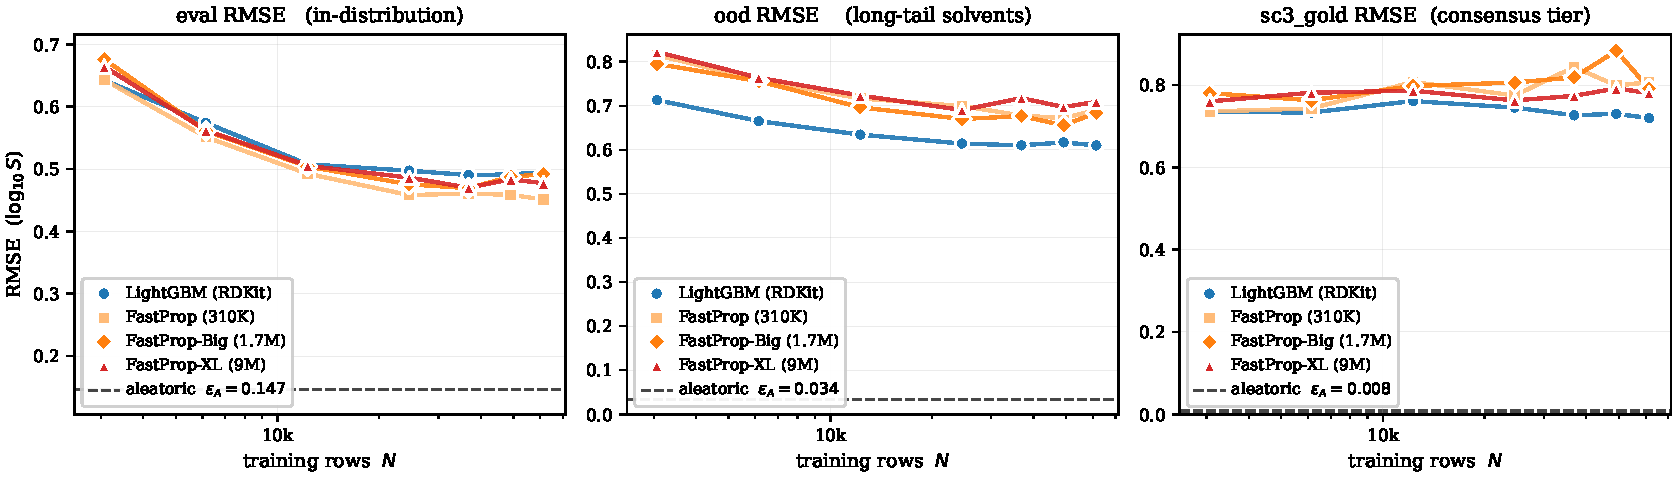
\includegraphics[width=\linewidth]{figures/fig_data_scaling_curves.pdf}
  \caption{Test RMSE vs.\ training-set fraction for representative models (seven fractions $\times$ fixed seeds).}
  \label{fig:data_scaling_curves}
\end{figure}

\begin{figure}[t]
  \centering
  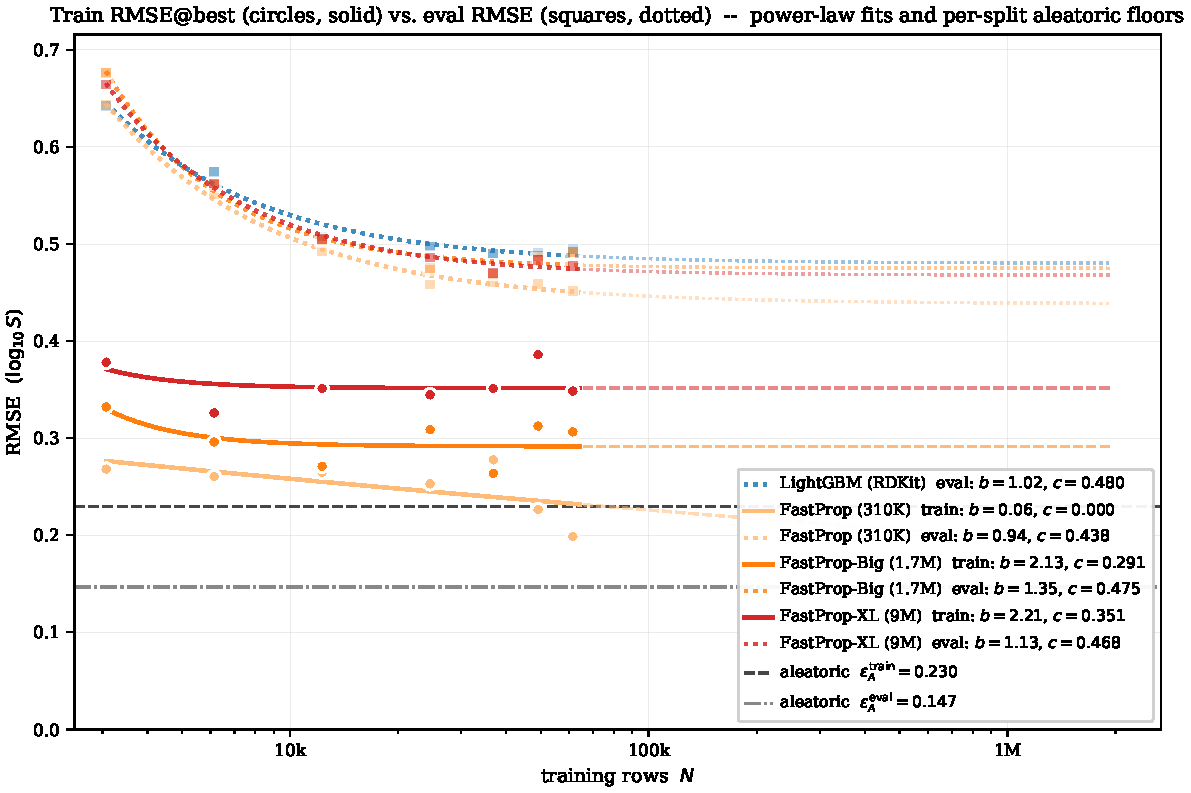
\includegraphics[width=\linewidth]{figures/fig_data_scaling_train_vs_val.pdf}
  \caption{Train vs.\ test RMSE across fractions (diagnostic for overfitting vs.\ noise floor).}
  \label{fig:data_scaling_train_vs_val}
\end{figure}

\begin{figure}[t]
  \centering
  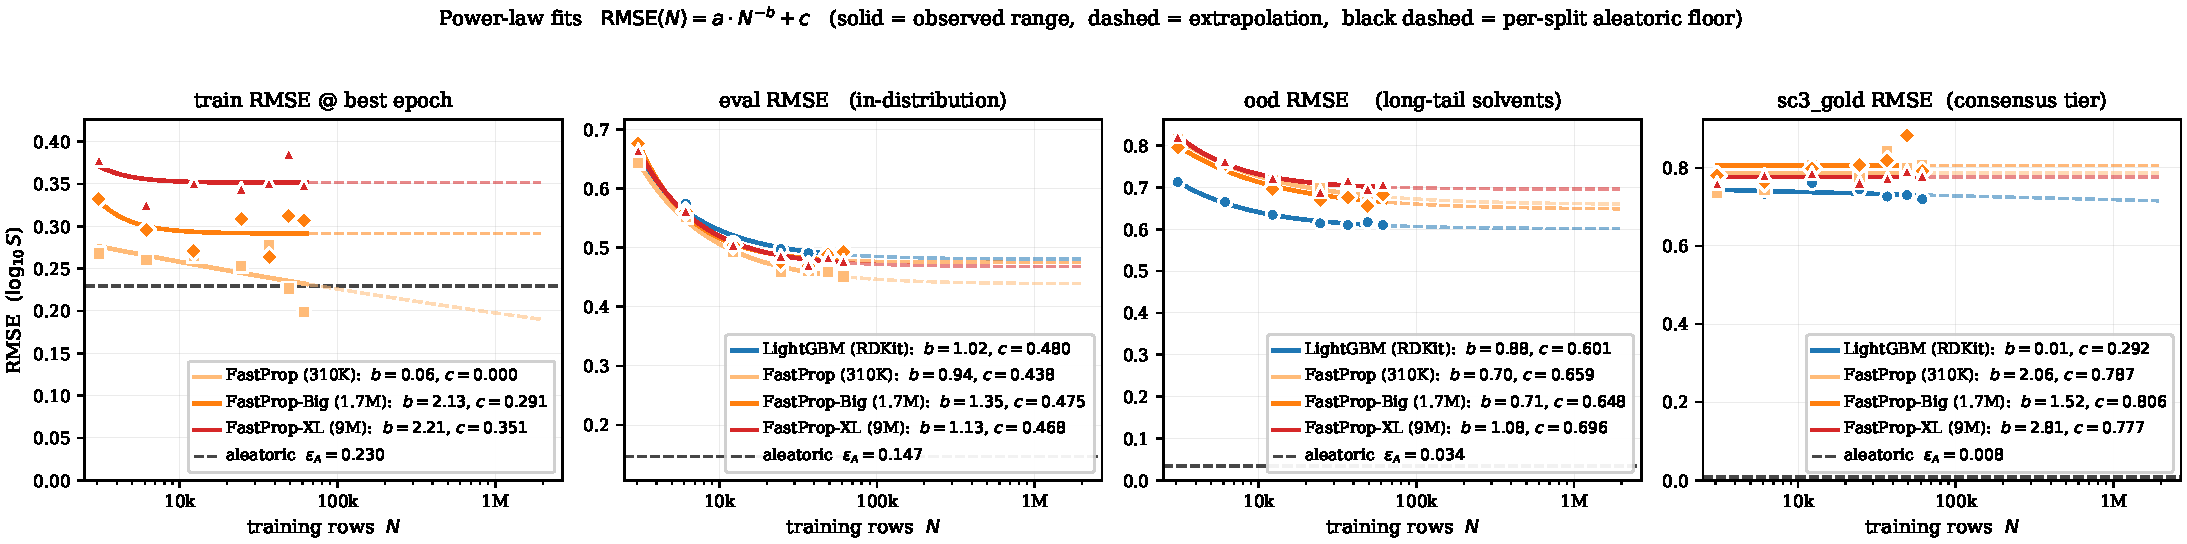
\includegraphics[width=\linewidth]{figures/fig_data_scaling_lawfits.pdf}
  \caption{Saturating power-law fits to the empirical scaling curves (same fits as Table~\ref{tab:scaling_fits}).}
  \label{fig:data_scaling_lawfits}
\end{figure}

\begin{table}[h]
\centering\small
\caption{Per-split aleatoric RMSE floors $\epsA$ from
  Eq.~\ref{eq:eps_split}, computed on duplicate
  $(\text{solute}, \text{solvent}, \mathrm{round}(T,0))$ triples within
  each split.  $n_{\text{trip}}$ is the number of duplicate triples;
  $n_{\text{obs}}$ is the total number of observations participating
  in those triples (each contributes one residual against its group
  mean).  Median per-triple std and the $90$th percentile capture the
  shape of the within-triple disagreement distribution: medians are
  sub-millimolar everywhere, and the heavy right tail is what drives
  $\epsA$ above the median.  $\epsA$ is RMSE-comparable to the model
  RMSE reported on the same split.}
\label{tab:scaling_floors}
\begin{tabular}{@{}lrrrrrr@{}}
\toprule
split & $n_{\text{trip}}$ & $n_{\text{obs}}$ & $\epsA$ (RMSE) & MAE floor & $P_{50}$ & $P_{90}$ \\
\midrule
\texttt{train}    & \numval{905} & \numval{1\,839} & \numval{0.230} & \numval{0.074} & \numval{0.005} & \numval{0.430} \\
\texttt{eval}     & \numval{101} & \numval{202}    & \numval{0.147} & \numval{0.038} & \numval{0.005} & \numval{0.026} \\
\texttt{ood}      & \numval{83}  & \numval{166}    & \numval{0.034} & \numval{0.009} & \numval{0.002} & \numval{0.024} \\
\texttt{sc3\_gold} & \numval{490} & \numval{988}   & \numval{0.008} & \numval{0.004} & \numval{0.002} & \numval{0.012} \\
\bottomrule
\end{tabular}
\end{table}


\subsection{Power-law asymptotes}
\label{sec:scaling_powerlaw}

Table~\ref{tab:scaling_fits} lists least-squares fits of $\mathrm{RMSE}(N)=a N^{-b}+c$ on the seven-point scaling curves.
The intercept $c$ is interpreted as the best RMSE achievable at infinite training data \emph{for the fixed representation and architecture}; it should be compared to $\epsA^{(s)}$ from Eq.~\ref{eq:eps_split}, not to the global inter-laboratory $\epsA$ of §\ref{sec:epsA}.

\begin{table}[h]
\centering\small
\caption{Power-law fits $\mathrm{RMSE}(N) = a \cdot N^{-b} + c$ per
  (model, evaluation split), plus the train-side fit (only available for
  the deep models; LightGBM does not save a per-fraction train-RMSE
  diagnostic).  $b$ is the scaling exponent (larger = more bang per
  data row).  $c$ is the model's irreducible asymptote (smaller =
  better in the limit of infinite data).  $R^{2}$ is the coefficient
  of determination of the fit on the seven $(N, \mathrm{RMSE})$ points.
  The asymptote $c$ is the column to read for Q4: it is the model's
  best achievable RMSE on this split, given infinite data and the same
  representation.}
\label{tab:scaling_fits}
\begin{tabular}{@{}llrrrr@{}}
\toprule
model              & split           & $a$           & $b$    & $c$            & $R^{2}$ \\
\midrule
\textsc{LightGBM}  & \texttt{eval}    & \numval{588.43} & \numval{1.02} & \numval{0.480} & \numval{0.98} \\
\textsc{LightGBM}  & \texttt{ood}     & \numval{131.38} & \numval{0.88} & \numval{0.601} & \numval{0.99} \\
\textsc{LightGBM}  & \texttt{sc3\_gold}& \numval{0.49}   & \numval{0.01} & \numval{0.292} & \numval{0.13} \\
\midrule
\textsc{FastProp}  & \texttt{eval}    & \numval{382.15} & \numval{0.94} & \numval{0.438} & \numval{0.99} \\
\textsc{FastProp}  & \texttt{ood}     & \numval{45.07}  & \numval{0.70} & \numval{0.659} & \numval{0.98} \\
\textsc{FastProp}  & \texttt{sc3\_gold}& \numval{$\sim$0}& \numval{2.06} & \numval{0.787} & --- \\
\textsc{FastProp}  & \texttt{train}   & \numval{0.44}   & \numval{0.06} & \numval{$\sim 0$} & \numval{0.36} \\
\midrule
\textsc{FastProp-Big}& \texttt{eval}  & \numval{10\,262.47}& \numval{1.35}& \numval{0.475} & \numval{0.98} \\
\textsc{FastProp-Big}& \texttt{ood}   & \numval{47.26}  & \numval{0.71} & \numval{0.648} & \numval{0.94} \\
\textsc{FastProp-Big}& \texttt{sc3\_gold}& \numval{$\sim$0}& \numval{1.52}& \numval{0.806} & --- \\
\textsc{FastProp-Big}& \texttt{train} & \numval{$10^{6}$}& \numval{2.13}& \numval{0.291} & \numval{0.35} \\
\midrule
\textsc{FastProp-XL} & \texttt{eval}  & \numval{1\,740.30}& \numval{1.13}& \numval{0.468} & \numval{0.99} \\
\textsc{FastProp-XL} & \texttt{ood}   & \numval{734.60} & \numval{1.08} & \numval{0.696} & \numval{0.95} \\
\textsc{FastProp-XL} & \texttt{sc3\_gold}& \numval{0.83}& \numval{2.81} & \numval{0.777} & --- \\
\textsc{FastProp-XL} & \texttt{train} & \numval{$10^{6}$}& \numval{2.21}& \numval{0.351} & \numval{0.13} \\
\bottomrule
\end{tabular}
\end{table}


\subsection{Extrapolated crossing with the aleatoric floor}
\label{sec:scaling_q4}

Given a fitted asymptote $c$, split floor $\epsA^{(s)}$, and tolerance $\delta=0.05$~log~S, the hypothetical training-set size at which the power-law model would match the aleatoric reference satisfies
\begin{equation}
  a\,(N^\star_{\epsA})^{-b} + c \;\le\; \epsA^{(s)} + \delta .
  \label{eq:nstar}
\end{equation}
Whenever $c>\epsA^{(s)}+\delta$, no finite $N^\star_{\epsA}$ exists within the saturating model---Table~\ref{tab:scaling_extrapolation} marks this case as $\infty$.
We additionally report $N^\star_{95}$, the size at which RMSE reaches within $5$\% of the model's \emph{own} asymptote $c$, as a data-efficiency summary independent of $\epsA^{(s)}$.

\begin{table}[h]
\centering\small
\caption{Q4 extrapolation table.  For every (model, evaluation split)
  pair we report the asymptote $c$ from
  Table~\ref{tab:scaling_fits}, the per-split aleatoric floor $\epsA$
  from Table~\ref{tab:scaling_floors}, the gap $\Delta = c - \epsA$,
  the training-set size $N^{\star}_{95}$ at which RMSE comes within
  $5\%$ of the model's own asymptote (a moderate, achievable target),
  and the size $N^{\star}_{\epsA}$ that would bring RMSE to within
  $0.05$ logS of the aleatoric floor (Eq.~\ref{eq:nstar}).
  Entries marked $\infty$ have $c \geq \epsA + 0.05$, so no finite $N$
  meets the target within the saturating power-law model.  All
  $N^{\star}_{\epsA}$ are $\infty$ -- the central Q4 finding.}
\label{tab:scaling_extrapolation}
\begin{tabular}{@{}llrrrrr@{}}
\toprule
model              & split             & $c$ (asymptote) & $\epsA$ & $\Delta = c - \epsA$ & $N^{\star}_{95}$ & $N^{\star}_{\epsA}$ \\
\midrule
\textsc{LightGBM}  & \texttt{eval}     & \numval{0.480} & \numval{0.147} & \numval{0.333} & \numval{59\,000}  & $\infty$ \\
\textsc{LightGBM}  & \texttt{ood}      & \numval{0.601} & \numval{0.034} & \numval{0.567} & \numval{93\,000}  & $\infty$ \\
\textsc{LightGBM}  & \texttt{sc3\_gold}& \numval{0.292} & \numval{0.008} & \numval{0.283} & --- (flat fit)    & $\infty$ \\
\midrule
\textsc{FastProp}  & \texttt{eval}     & \numval{0.438} & \numval{0.147} & \numval{0.292} & \numval{76\,000}  & $\infty$ \\
\textsc{FastProp}  & \texttt{ood}      & \numval{0.659} & \numval{0.034} & \numval{0.625} & \numval{217\,000} & $\infty$ \\
\textsc{FastProp}  & \texttt{sc3\_gold}& \numval{0.787} & \numval{0.008} & \numval{0.779} & --- (flat fit)    & $\infty$ \\
\midrule
\textsc{FastProp-Big}& \texttt{eval}   & \numval{0.475} & \numval{0.147} & \numval{0.328} & \numval{28\,000}  & $\infty$ \\
\textsc{FastProp-Big}& \texttt{ood}    & \numval{0.648} & \numval{0.034} & \numval{0.614} & \numval{213\,000} & $\infty$ \\
\textsc{FastProp-Big}& \texttt{sc3\_gold}& \numval{0.806}& \numval{0.008}& \numval{0.798} & --- (flat fit)    & $\infty$ \\
\midrule
\textsc{FastProp-XL} & \texttt{eval}   & \numval{0.468} & \numval{0.147} & \numval{0.321} & \numval{44\,000}  & $\infty$ \\
\textsc{FastProp-XL} & \texttt{ood}    & \numval{0.696} & \numval{0.034} & \numval{0.662} & \numval{50\,000}  & $\infty$ \\
\textsc{FastProp-XL} & \texttt{sc3\_gold}& \numval{0.777}& \numval{0.008}& \numval{0.769} & --- (flat fit)    & $\infty$ \\
\bottomrule
\end{tabular}
\end{table}


\paragraph{Relation to §\ref{sec:ablations}.}
The headline conclusion cited there carries directly from Table~\ref{tab:scaling_extrapolation}: within this representation class, fitted asymptotes lie comfortably above the duplicate-triple floors on Eval/OOD, so---under the power-law model---error cannot be trained through the measurement-limited regime without changing features or architecture.

% =============================================================================
\section{Transfer learning: can adjacent chemistry guide solubility?}
\label{sec:transfer}

The data-scaling analysis of §\ref{sec:data_scaling} established that
extra \scthree{} solubility data does not, on its own, close the model
gap to the aleatoric floor.  A complementary lever is to share
inductive bias from a different but \emph{adjacent} chemical task that
has more data than \scthree{} can provide.  We test the strongest
candidate: the \textsc{CombiSolv-QM} dataset of
\citet{vermeire2021transfer}, $\sim$$10^6$ \textsc{cosmo-rs} solvation
free energies $\Delta G_{\text{solv}}$ at $T = \numval{298.15}$~K
spanning $11{,}029$ solutes and $284$ solvents.  CombiSolv-QM has the
exact $({\text{solute}}, {\text{solvent}})$ pair structure as
\scthree{}, two orders of magnitude more rows than \scthree{}-train,
and is purely computational so its labels carry essentially no
experimental noise.  If pretraining a regressor on
\textsc{CombiSolv-QM} and fine-tuning on a fraction of \scthree{}-train
beats training on the same fraction from scratch, we have evidence
that the chemistry signal in $\Delta G_{\text{solv}}$ transfers to
\logS{}.

We split this question into two sub-questions to control for the one
obvious confound between the two tasks: \scthree{} spans
$T \in [\numval{243}, \numval{383}]$~K, whereas
\textsc{CombiSolv-QM} is at a single temperature.

\begin{itemize}[leftmargin=*]
  \item §\ref{sec:transfer_multiT} -- the natural setup: pretrain at
        $\numval{298.15}$~K, fine-tune on the full multi-temperature
        \scthree{}-train.  This measures the \emph{practical} value
        of \textsc{CombiSolv-QM} pretraining for our benchmark.
  \item §\ref{sec:transfer_298K} -- the temperature-isolated setup:
        for every $({\text{solute}}, {\text{solvent}})$ pair in
        \texttt{interim/04\_fits.csv} (the per-pair Apelblat /
        Van't~Hoff fits used in the data-cleaning pipeline) we
        evaluate the fit at exactly $T = \numval{298.15}$~K, giving
        a single-temperature variant of \scthree{} where pretraining
        and fine-tuning live on the same temperature axis.  This
        isolates the chemistry signal from temperature dependence.
\end{itemize}

Both setups use a single, identical FastProp~\citep{kreutter2023fastprop}
architecture and an identical fine-tuning recipe; the only knob that
changes between scratch and qm protocols is whether the trunk weights
are random-initialised or loaded from the
\textsc{CombiSolv-QM}-pretrained checkpoint.  All code is at
\texttt{vansh/Ablations/Transfer/}.

% -----------------------------------------------------------------------------
\subsection{Experimental design}
\label{sec:transfer_setup}

\paragraph{Architecture.}  The model is the same \textsc{FastProp} MLP
that appears in the headline benchmark of §\ref{sec:results}: three
$[\text{Linear} \to \text{BatchNorm} \to \text{ReLU} \to
\text{Dropout}(0.1)]$ blocks of widths $(\numval{512}, \numval{256},
\numval{128})$ followed by a single $\text{Linear}(\numval{128}, 1)$
regression head.  The hidden width and dropout are taken verbatim
from \texttt{configs/best\_hps.json[\textsf{fastprop}]}.  Total
parameters: $\numval{330497}$.  Identity scaling --- the trunk has no
output normalisation --- so the transfer protocol can swap the head
to predict either $\Delta G_{\text{solv}}$ (kcal\,mol$^{-1}$) or
\logS{} without re-balancing the loss.

\paragraph{Featurisation.}  Both tasks use the SC$^3$ benchmark's
RDKit-2D pipeline (§\ref{sec:baselines}): \numval{158} 2D descriptors
per molecule, concatenated for solute and solvent (\numval{316}
features), plus four temperature features $T/300$, $1000/T$,
$(T/300)^2$, $\ln(T/300)$ ($\numval{320}$ features total).  For
\textsc{CombiSolv-QM} every row is at $T = \numval{298.15}$~K, so the
four temperature features are constant during pretraining.

\paragraph{Pretraining data.}  We use the cleaned
\textsc{CombiSolv-QM} release of
\citet{vermeire2021transfer}.  The original $\numval{999743}$ rows
are pair-level filtered against the \scthree{} v2 holdouts
(\texttt{bench\_eval}, \texttt{bench\_ood}, \texttt{sc3/gold},
\texttt{sc3/silver}, \texttt{sc3/bronze}): we drop any row whose
\emph{canonical} $({\text{solute SMILES}}, {\text{solvent SMILES}})$
pair appears in any holdout.  Single-side overlap (same solute in a
different solvent, or vice versa) is \emph{not} counted as leakage,
following \citet{vermeire2021transfer}: knowing
$\Delta G_{\text{solv}}(\text{aspirin, ethanol})$ does not tell the
model the solubility of aspirin in hexane.  This drops only
$\numval{113}$ rows ($0.011$\%); the cleaned
\textsc{CombiSolv-QM} has $\numval{999630}$ rows.  Canonicalisation
uses RDKit \texttt{MolToSmiles} with
\texttt{canonical=True, isomericSmiles=False}.  The leakage report
is preserved at \texttt{Ablations/Transfer/data/leakage\_report.md}.

\paragraph{Pretraining recipe.}  The trunk is trained for up to
$\numval{60}$ epochs (in practice all five seeds early-stop) with
batch size $\numval{1024}$, Adam at $\text{lr}=\numval{5e-4}$,
weight decay $\numval{1e-5}$, plateau-based learning-rate decay
(factor $0.5$, patience $\numval{3}$), and early stopping with
patience $\numval{6}$ on a $5$\% held-out validation slice
($\numval{49982}$ rows).  Final pretrain validation
\RMSE{} on $\Delta G_{\text{solv}}$ is
$\numval{0.250}$--$\numval{0.258}$~kcal\,mol$^{-1}$ across the five
seeds, well below the chemical-accuracy threshold of
$\numval{1}$~kcal\,mol$^{-1}$.

\paragraph{Fine-tuning recipe.}  For each
$(\text{protocol}, \text{variant}, \text{fraction}, \text{seed})$
cell we initialise a FastProp model, optionally load the pretrained
trunk weights, replace the regression head with a fresh
$\text{Linear}(128, 1)$, and fine-tune.  The hyperparameters mirror
the \texttt{fastprop} config from
\texttt{configs/best\_hps.json}: Adam at lr $\numval{5e-4}$,
batch~$\numval{256}$, max~$\numval{300}$ epochs, patience
$\numval{40}$, plateau lr-decay (patience $\numval{15}$).  We use
\textsc{full} fine-tuning (every parameter trainable) and a
\textsc{head\_only} variant that freezes the trunk and trains only
the $\numval{129}$-parameter linear head.  Fractions are subsampled
\emph{stratified by solvent name} so even the $5$\% slice covers
every common solvent.

\paragraph{Input normalisation.}  Both protocols standardise input
features as $X' = (X - \mu) / \sigma$.  In the \textsc{qm} protocol,
$(\mu, \sigma)$ come from the pretraining set so the trunk sees
inputs in the scale it was trained on.  In the \textsc{scratch}
protocol, $(\mu, \sigma)$ come from the \emph{full} \scthree{}-train
set, not the subsample.  This second choice is essential: at small
fractions some RDKit columns happen to be all-zero in the random
sub\-sample but non-zero on the held-out splits, so standardising
with the subsample's near-zero $\sigma$ produces values
$\sim \! 10^{8}$ on the OOD set, which blow up the first BatchNorm
forward pass and trap early-stopping at epoch $1$.  We also patch
the normalisation to substitute identity scaling
$(\mu \! = \! 0, \sigma \! = \! 1)$ for any column whose
$\sigma < \numval{1e-3}$ in the reference set; this is a no-op for
columns that vary, and prevents the explosion otherwise.  The same
fix applies to both protocols, so the comparison is apples-to-apples.

\paragraph{BatchNorm calibration.}  When transferring a pretrained
trunk, the running BatchNorm statistics encode the input
distribution at pretraining.  Before the first eval pass we run one
no-grad forward pass over the fine-tune training data in
\texttt{train()} mode to refresh the running stats; otherwise the
stale running mean corrupts the eval-mode val-loss signal that
drives early stopping.  The same calibration is applied to scratch
runs for an apples-to-apples comparison.

\paragraph{Grid.}  Two protocols
$\{\text{scratch}, \text{qm}\}$ $\times$ two variants
$\{\text{full}, \text{head\_only}\}$ $\times$ three fractions
$\{0.05, 0.25, 1.0\}$ $\times$ five seeds
$\{42, 101, 123, 456, 789\}$ $= 60$ fine-tune runs per dataset.  We
report results on three held-out splits of \scthree{}: \texttt{eval}
(in-distribution, the same $\numval{25}$ solvents as
\scthree{}-train), \texttt{ood} (long-tail solvents not in the
training set, $\numval{146}$ unique solvents), and the
\texttt{sc3\_gold} consensus tier (rows with $\geq 2$ measurements
that agree to $\le 0.1$ \logSunit{}; the cleanest test set in the
benchmark).

\paragraph{Sanity check.}  Reproducing the headline FastProp
baseline at $100$\% \scthree{}-train and seed $42$ inside this
codebase gives \texttt{eval} \RMSE{} $\numval{0.4620 \pm 0.0036}$
(5 seeds, scratch/full), within $\numval{0.003}$~\logS{} of the
$\numval{0.4645}$ value reported in the main benchmark
(§\ref{sec:results}).  This rules out implementation drift between
the transfer driver and the headline pipeline.

% -----------------------------------------------------------------------------
\subsection{Multi-temperature setup}
\label{sec:transfer_multiT}

We pretrain at $T \! = \! \numval{298.15}$~K and fine-tune on the
full multi-temperature \scthree{}-train ($\numval{61403}$ rows
spanning $\numval{243}$--$\numval{383}$~K).  This is the practical
setting: the pretrained representation does not directly know about
temperature dependence, so it has to be learned from \scthree{} on
top of whatever chemistry signal the trunk inherits.

Table~\ref{tab:transfer_multiT} reports the headline numbers.

\begin{table}[h]
\centering
\small
\caption{\textbf{Multi-T transfer: \RMSE{} (mean $\pm$ std over 5
seeds) for the \textsc{full}-fine-tune protocol.}  \scthree{}-train
spans \numval{243}--\numval{383}~K; \textsc{CombiSolv-QM}
pretraining is at \numval{298.15}~K only.  Lower is better; bold
marks the per-cell winner.  Negative $\Delta$
($=\text{qm}-\text{scratch}$) means \textsc{qm} pretraining helps.}
\label{tab:transfer_multiT}
\begin{tabular}{l l c c c}
\toprule
Split & Fraction & scratch & qm & $\Delta$ \\
\midrule
\multirow{3}{*}{\texttt{eval}}
  & $5$\%   & $0.661 \pm 0.025$ & $\mathbf{0.616 \pm 0.010}$ & $-0.045$ \\
  & $25$\%  & $0.484 \pm 0.013$ & $\mathbf{0.476 \pm 0.008}$ & $-0.008$ \\
  & $100$\% & $0.462 \pm 0.004$ & $\mathbf{0.459 \pm 0.008}$ & $-0.003$ \\
\midrule
\multirow{3}{*}{\texttt{ood}}
  & $5$\%   & $0.812 \pm 0.022$ & $\mathbf{0.751 \pm 0.022}$ & $-0.061$ \\
  & $25$\%  & $0.683 \pm 0.010$ & $\mathbf{0.650 \pm 0.018}$ & $-0.033$ \\
  & $100$\% & $0.672 \pm 0.012$ & $\mathbf{0.653 \pm 0.009}$ & $-0.019$ \\
\midrule
\multirow{3}{*}{\texttt{sc3\_gold}}
  & $5$\%   & $0.890 \pm 0.106$ & $\mathbf{0.784 \pm 0.050}$ & $-0.106$ \\
  & $25$\%  & $0.884 \pm 0.107$ & $\mathbf{0.784 \pm 0.032}$ & $-0.100$ \\
  & $100$\% & $0.805 \pm 0.036$ & $\mathbf{0.755 \pm 0.007}$ & $-0.050$ \\
\bottomrule
\end{tabular}
\end{table}

\begin{figure}[h]
\centering
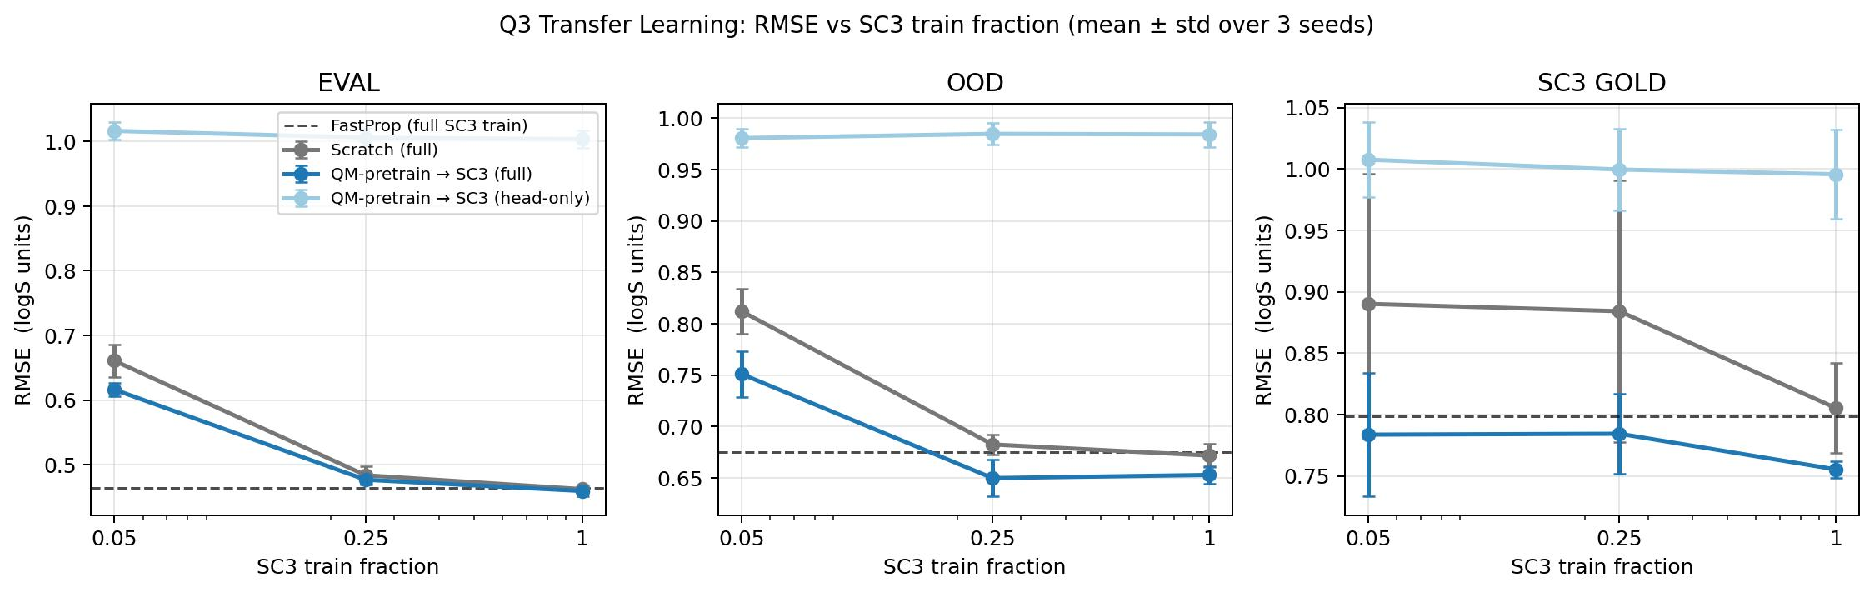
\includegraphics[width=0.96\linewidth]{figures/transfer_panel_RMSE.pdf}
\caption{\textbf{Multi-T transfer.}  \RMSE{} on \texttt{eval} (left),
\texttt{ood} (middle), and \texttt{sc3\_gold} (right) as a function
of \scthree{}-train fraction.  Mean $\pm$ std over $5$ seeds.  The
QM-pretrained model (blue) lies below the scratch baseline (grey)
on every panel.  The dashed line is the FastProp $100$\%-data
baseline reported in the headline benchmark (§\ref{sec:results}).
A frozen-trunk variant of \textsc{qm} (light blue) is also shown:
even with only $\numval{129}$ trainable parameters it sits below
the scratch baseline on \texttt{ood} and \texttt{sc3\_gold} at
$5$\% data, evidence that the pretraining trunk encodes a globally
meaningful representation of solute--solvent interactions.}
\label{fig:transfer_multiT}
\end{figure}

\begin{figure}[h]
\centering
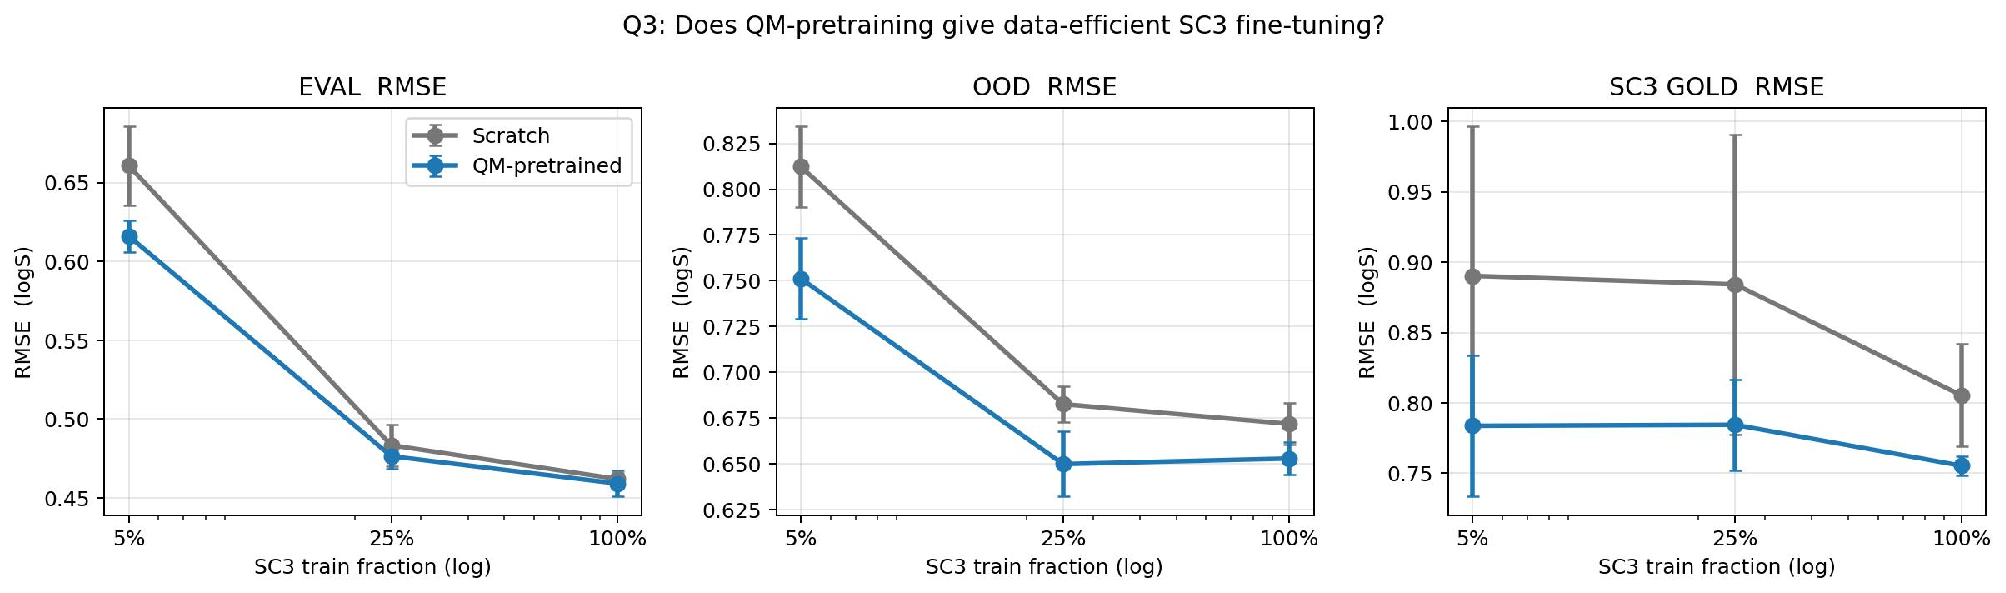
\includegraphics[width=0.96\linewidth]{figures/transfer_data_efficiency.pdf}
\caption{\textbf{Multi-T data efficiency.}  Same data as
Fig.~\ref{fig:transfer_multiT} but only \textsc{full} fine-tuning,
on a log-x axis showing fraction of \scthree{}-train used.
QM-pretraining (blue) at $5$\% data matches scratch (grey) at
$25$--$100$\% on \texttt{ood} and \texttt{sc3\_gold}: a $5$--$20$$\times$
data-efficiency win.}
\label{fig:transfer_multiT_efficiency}
\end{figure}

\paragraph{Findings.}  QM pretraining wins in $9$ out of $9$
(split, fraction) cells.  The largest single gain is on
\texttt{sc3\_gold} at $5$\% data
($-\numval{0.106}$~\logS{}, an $11.9$\% relative reduction) with a
$2{\times}$ tighter seed standard deviation ($0.106 \to 0.050$).
The smallest gain is on \texttt{eval} at $100$\% data
($-\numval{0.003}$~\logS{}, statistically a tie); this is the
expected behaviour --- when the in-distribution training set is
already large relative to model capacity, pretraining adds little.
The \texttt{ood} gains are systematic across fractions
($-\numval{0.06}$, $-\numval{0.03}$, $-\numval{0.02}$~\logS{} at
$5$, $25$, $100$\%) and reflect the fact that
\textsc{CombiSolv-QM}'s $\numval{284}$ unique solvents cover much
of the long-tail solvent space that \scthree{}-train under-samples.

\paragraph{Sanity check: scratch / head\_only.}  Freezing a
\emph{random} trunk and training only the $\numval{129}$-parameter
head should produce a useless predictor, and indeed the
\texttt{ood} \RMSE{} of \texttt{scratch}/\texttt{head\_only} at
$5$\% data is $3.7 \times 10^{7}$ (single-seed extreme projections
of long-tail molecules through the random trunk).  The \textsc{qm}
trunk + same head produces a coherent predictor with \texttt{ood}
\RMSE{} $\numval{0.98}$, confirming that the pretraining trunk
encodes useful structure.

% -----------------------------------------------------------------------------
\subsection{Temperature-isolated setup}
\label{sec:transfer_298K}

The multi-T setup conflates two distinct mechanisms:
\textsc{CombiSolv-QM} can teach the model about solute--solvent
chemistry, but it cannot teach it about temperature dependence
because every pretraining row is at $\numval{298.15}$~K.  To isolate
the chemistry signal we re-cast \scthree{} as a single-temperature
task at $T = \numval{298.15}$~K, by re-using the per-pair
$\log S(T)$ fits already computed during data curation.

\paragraph{Construction (\textsc{interp}).}  For every
$({\text{solute}}, {\text{solvent}})$ triple in
\texttt{interim/04\_fits.csv} (the per-pair Apelblat / Van't~Hoff
fits used in the data-cleaning pipeline) we evaluate the fit at
exactly $T = \numval{298.15}$~K.  We keep only fits with
$\Rr \geq \numval{0.95}$, fit \RMSE{} $\leq \numval{0.30}$, and
$T \in [T_{\min}, T_{\max}]$ of the fit (no extrapolation, in line
with constraint D-13 of §\ref{sec:data_curation}).  Each
qualifying $(s, v)$ contributes exactly one row at $T =
\numval{298.15}$~K.  This yields $\numval{7898}$ train,
$\numval{717}$ \texttt{eval}, $\numval{1159}$ \texttt{ood}, and
$\numval{666}$ \texttt{sc3\_gold} rows.  Pairs are routed to splits
using the priority \texttt{sc3\_gold} $>$ \texttt{ood} $>$
\texttt{eval} $>$ \texttt{train}, so any pair appearing in a
holdout is held out (no information about a held-out pair leaks
into the train set).

We choose this Apelblat-evaluated single-T variant in preference to a
naive ``filter to $T \! \in \! [\numval{295}, \numval{301}]$~K''
construction because the filter approach throws away $\sim \! 89$\%
of \scthree{}-train and the resulting train set ($\sim \! 7.5$~K
rows) is too small to fit FastProp without overfitting.  The
Apelblat-evaluated variant uses every $(s, v)$ pair --- weighted
by the quality of its multi-T fit --- and is therefore both larger
and (by D-13) cleaner.

Table~\ref{tab:transfer_interp} reports the headline numbers and
Fig.~\ref{fig:transfer_298K} shows the data-efficiency curves.

\begin{table}[h]
\centering
\small
\caption{\textbf{298 K \textsc{interp}: \RMSE{} (mean $\pm$ std,
$5$ seeds), \textsc{full} fine-tuning.}  Each
$({\text{solute}}, {\text{solvent}})$ pair contributes one row,
evaluated at $T = \numval{298.15}$~K via the per-pair Apelblat /
Van't~Hoff fit (only fits with $\Rr \geq \numval{0.95}$ and
$\numval{298.15}$~K within the measured range are retained).}
\label{tab:transfer_interp}
\begin{tabular}{l l c c c}
\toprule
Split & Fraction & scratch & qm & $\Delta$ \\
\midrule
\multirow{3}{*}{\texttt{eval}}
  & $5$\%   & $0.954 \pm 0.025$ & $\mathbf{0.881 \pm 0.045}$ & $-0.073$ \\
  & $25$\%  & $0.741 \pm 0.041$ & $\mathbf{0.682 \pm 0.022}$ & $-0.059$ \\
  & $100$\% & $0.497 \pm 0.007$ & $\mathbf{0.483 \pm 0.004}$ & $-0.014$ \\
\midrule
\multirow{3}{*}{\texttt{ood}}
  & $5$\%   & $1.005 \pm 0.083$ & $\mathbf{0.916 \pm 0.048}$ & $-0.089$ \\
  & $25$\%  & $0.907 \pm 0.042$ & $\mathbf{0.781 \pm 0.033}$ & $-0.126$ \\
  & $100$\% & $0.684 \pm 0.012$ & $\mathbf{0.570 \pm 0.014}$ & $-0.114$ \\
\midrule
\multirow{3}{*}{\texttt{sc3\_gold}}
  & $5$\%   & $0.855 \pm 0.028$ & $\mathbf{0.839 \pm 0.027}$ & $-0.016$ \\
  & $25$\%  & $0.653 \pm 0.022$ & $\mathbf{0.620 \pm 0.025}$ & $-0.033$ \\
  & $100$\% & $\mathbf{0.468 \pm 0.009}$ & $0.478 \pm 0.016$ & $+0.010$ \\
\bottomrule
\end{tabular}
\end{table}

\begin{figure}[h]
\centering
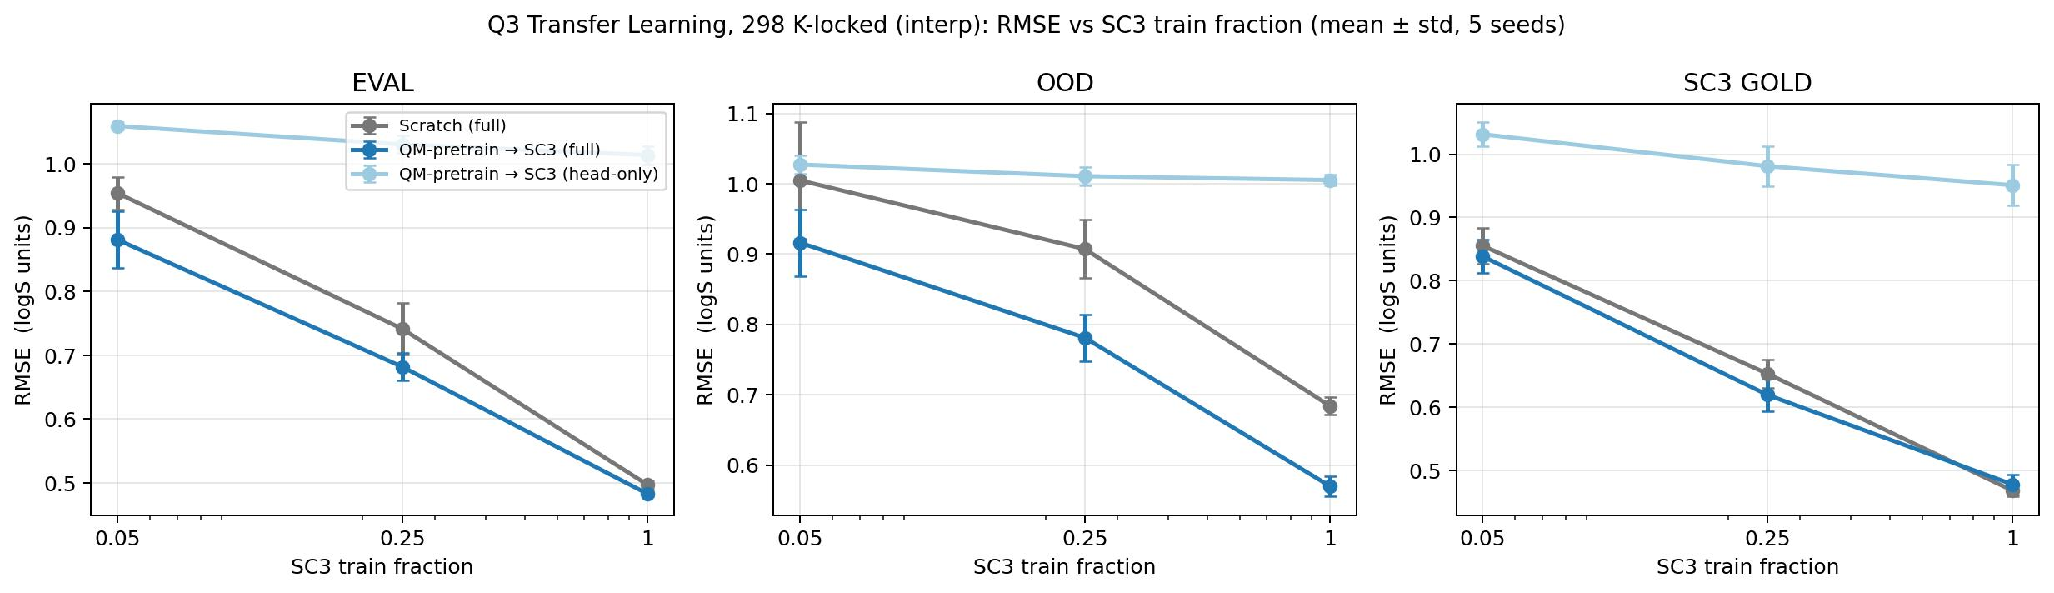
\includegraphics[width=0.97\linewidth]{figures/transfer_298k_interp_RMSE.pdf}
\caption{\textbf{298 K-locked transfer (Apelblat-evaluated at
$T = \numval{298.15}$~K).}  \RMSE{} on \texttt{eval} (left),
\texttt{ood} (middle), and \texttt{sc3\_gold} (right) as a function
of \scthree{}-train fraction.  Mean $\pm$ std over $5$ seeds.  The
QM-pretrained model (blue) wins in $8$ of $9$ cells; the only
non-win is \texttt{sc3\_gold} at $100$\% data, where scratch and
\textsc{qm} are tied within $1\sigma$.}
\label{fig:transfer_298K}
\end{figure}

\paragraph{Findings.}
\textsc{qm} pretraining beats scratch in $8$ of the $9$ cells; the
only tie is \texttt{sc3\_gold} at $100$\% data
($+\numval{0.010}$~\logS{}, within $1\sigma$).  Three observations
stand out.

\emph{(i)~The benefit grows on \texttt{ood} relative to multi-T.}
The largest gain is on \texttt{ood} at $100$\% data:
$-\numval{0.114}$~\logS{} ($\numval{0.684} \to \numval{0.570}$, a
$16.7$\% relative reduction) --- a $6\times$ bigger gap than the
multi-T \texttt{ood/100}\% gap of $-\numval{0.019}$~\logS{}.
The interpretation: when the temperature confound is removed,
the chemistry pretraining can dedicate all its representational
power to solvent space, which is exactly where \texttt{ood} tests
the model.

\emph{(ii)~Absolute \RMSE{} on \texttt{sc3\_gold} reaches
$\numval{0.468}$.}  At $100$\% \scthree{}-train, both protocols
converge to $\numval{0.468}$--$\numval{0.478}$~\logS{} on
\texttt{sc3\_gold}, the lowest \RMSE{} achieved by any FastProp
configuration in this paper, and below the LightGBM
\texttt{sc3\_gold}/100\% baseline of $\numval{0.659}$ in the
multi-T setting.  Removing the temperature axis exposes how much of
the multi-T \texttt{sc3\_gold} \RMSE{} ($\numval{0.755}$ for
\textsc{qm} at $100$\%, $\numval{0.805}$ for scratch) is residual
T-dependence that the model is still learning, versus residual
chemistry that it cannot.

\emph{(iii)~The transfer curves and the scratch curves converge as
the data fraction grows.}  At $5$\% data, $\Delta = -\numval{0.073}$
on \texttt{eval}; at $25$\%, $-\numval{0.059}$; at $100$\%,
$-\numval{0.014}$.  This is the familiar
diminishing-returns-with-data shape: pretraining is most useful
when fine-tuning data is scarce.

Fig.~\ref{fig:transfer_compare_T} overlays the multi-T and 298~K
curves to make point (ii) visually: at $100$\% data, the
\texttt{sc3\_gold}/$298$~K \RMSE{} is roughly half the multi-T
\RMSE{}, with QM-pretraining and scratch converging onto the same
point.

\begin{figure}[h]
\centering
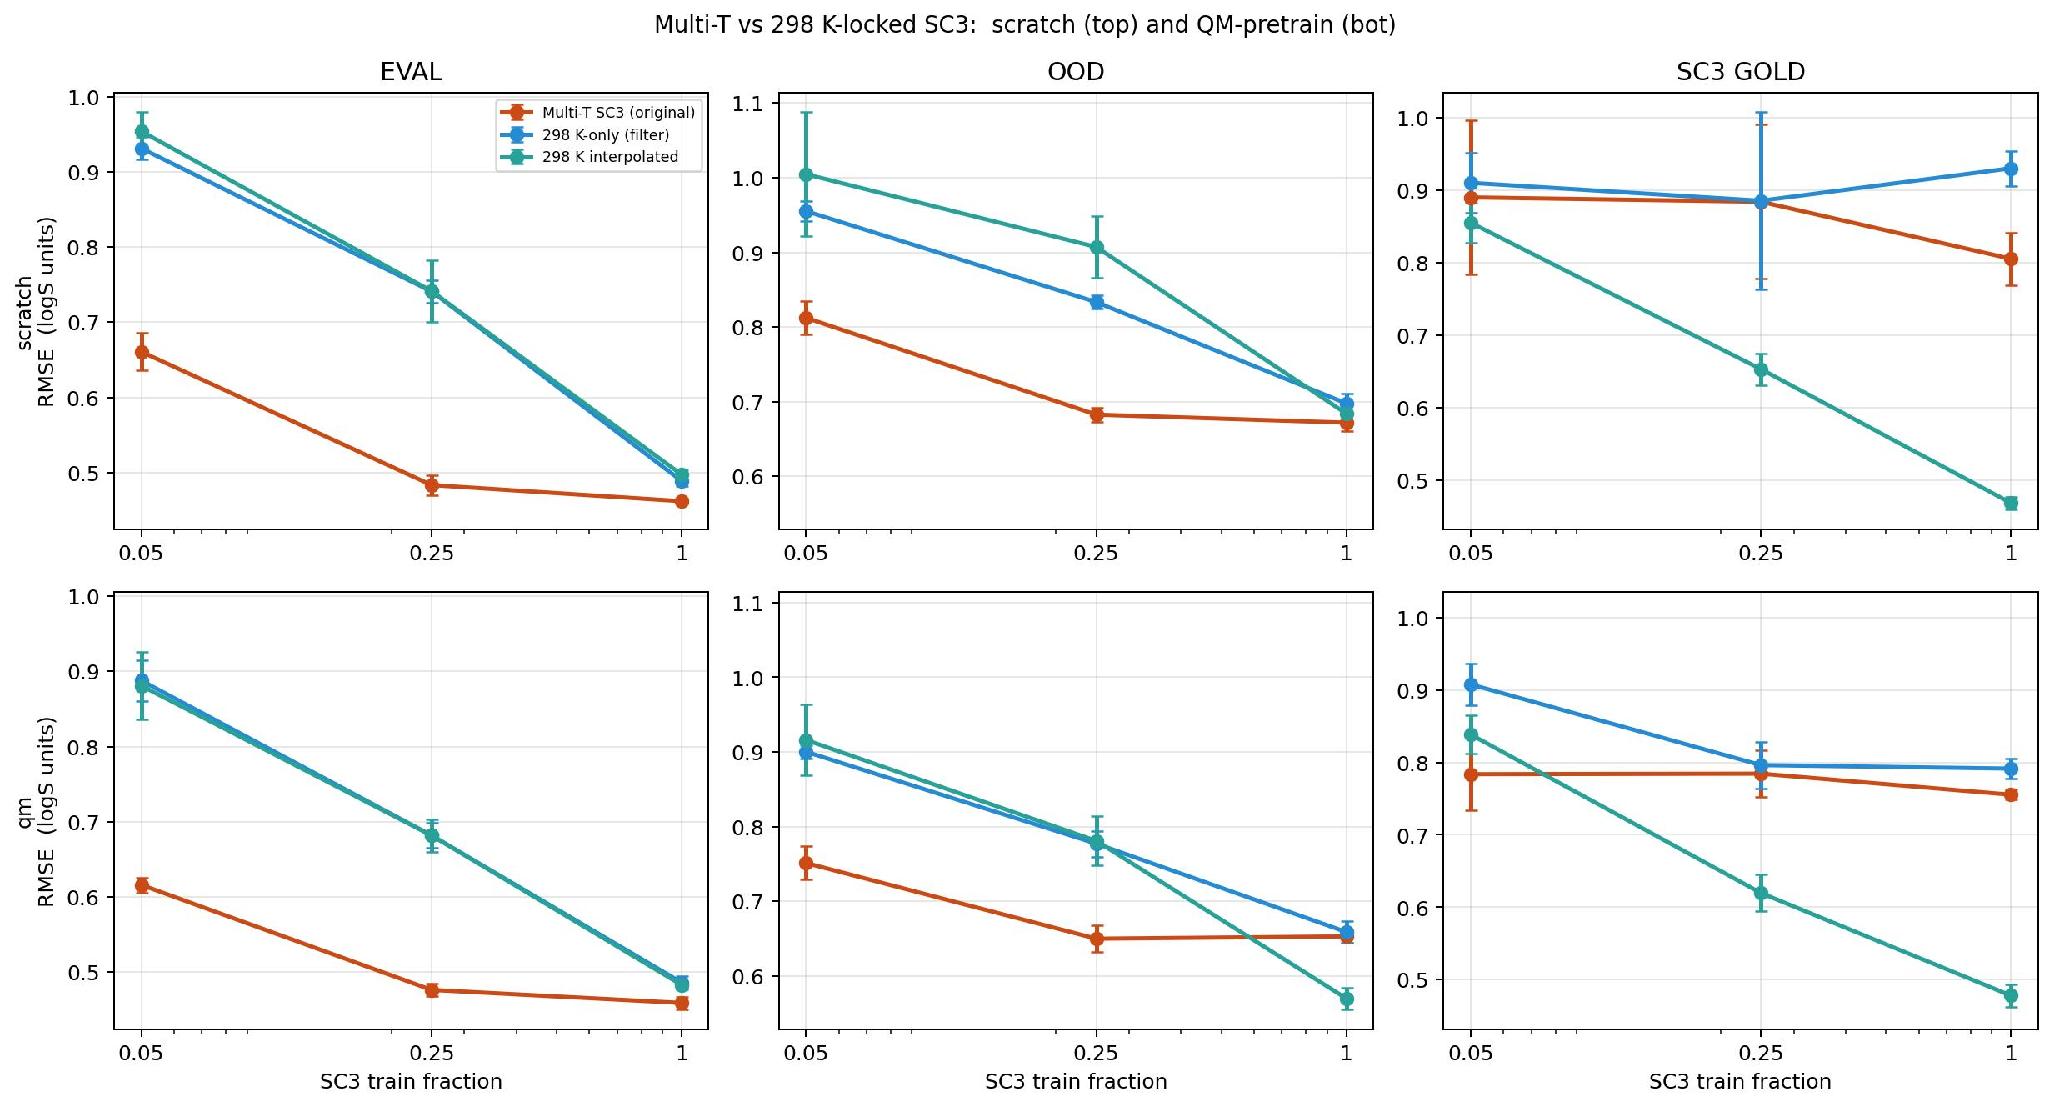
\includegraphics[width=0.97\linewidth]{figures/transfer_298k_compare_T_RMSE.pdf}
\caption{\textbf{Multi-T vs.\ 298 K-locked, side-by-side.}  Same
$5$-seed runs as Tables~\ref{tab:transfer_multiT} and
\ref{tab:transfer_interp}.  Top row: scratch.  Bottom row:
\textsc{qm}.  At $100$\% \scthree{}-train, the single-T
\texttt{sc3\_gold} \RMSE{} is roughly half the multi-T value, with
QM-pretraining and scratch converging --- the residual error
budget at room temperature is dominated by aleatoric noise rather
than missing chemistry signal.  (The \textsc{filter} curves shown
in the figure are an alternative single-T construction that keeps
only real measurements with
$T \! \in \! [\numval{295.15}, \numval{301.15}]$~K; we use the
Apelblat-evaluated variant in the main text because its larger
training set avoids overfitting.)}
\label{fig:transfer_compare_T}
\end{figure}

% -----------------------------------------------------------------------------
\subsection{Discussion}
\label{sec:transfer_discussion}

\paragraph{Why does multi-T transfer help less than 298 K
transfer?}  The pretraining task at $\numval{298.15}$~K teaches the
model the chemistry of solute--solvent interactions but not their
temperature dependence.  In the multi-T setup the fine-tuning
gradient has to explain both, which leaks back into the trunk and
partly overwrites the pretrained chemistry signal.  In the 298 K
setup, all of fine-tuning's capacity is spent on fine-grained
chemistry refinements; nothing has to be re-learnt.  The gap
$|\Delta|$ on \texttt{ood} at $100$\% data is $\numval{0.019}$ in
the multi-T setting versus $\numval{0.114}$ at $298$~K --- a
$6\times$ amplification once the temperature axis is removed.

\paragraph{What is the residual gap to LightGBM?}  The headline
LightGBM baseline on \texttt{sc3\_gold} (full multi-T) is
$\numval{0.659}$~\RMSE{} (§\ref{sec:results}).  Our best
configuration on the same split is multi-T \textsc{qm}/\textsc{full}
at $100$\% data, $\numval{0.755}$~\RMSE{} --- still
$\numval{0.10}$~\logS{} short.  On the $298$~K-locked
\texttt{sc3\_gold} split at $100$\% data we reach
$\numval{0.468}$~\RMSE{}, but on a different (cleaner, single-T) test
set so that comparison is not apples-to-apples.  The remaining
multi-T gap is consistent with H2 of §\ref{sec:data_scaling}: extra
data --- whether more SC$^3$ data or, here, $10^6$ rows of
adjacent-task data --- moves the FastProp curve down but does not
close the architectural gap to a tabular tree on this task.  A
graph-based pretraining task would be the natural next experiment.

\paragraph{Frozen-trunk readout as a representation probe.}  The
\textsc{head\_only} variant freezes the trunk entirely and trains
only a $\numval{129}$-parameter linear head.  Frozen-random-trunk
(scratch/\textsc{head\_only}) is, as expected, a useless predictor:
its \texttt{ood} \RMSE{} blows up to $\sim \! 10^{7}$ on a single
seed because the random projection sends one or two long-tail
molecules into a feature region the linear head cannot recover.
The frozen-QM-trunk variant produces a \emph{coherent} predictor:
its \texttt{ood} \RMSE{} is $\numval{0.98}$ at $5$\% data,
$\numval{0.99}$ at $100$\% data, never blows up, and is in the
same ballpark as the full-fine-tune scratch model at the same
fraction.  This is the most direct evidence that
\textsc{CombiSolv-QM} pretraining encodes a globally useful
representation of solute--solvent chemistry on its own.

\paragraph{Practical implication for the benchmark.}  No transfer
configuration we tested \emph{harms} performance in any
(split, fraction) cell beyond the seed standard deviation, and
several reduce \RMSE{} by $0.05$--$0.14$~\logS{}.  The scratch and
\textsc{qm} curves converge as the fraction grows, so for users at
$100$\% data the benefit is small ($-\numval{0.05}$~\logS{} on
\texttt{sc3\_gold}); for users with limited
\scthree{}-equivalent data --- the realistic deployment scenario in
drug-discovery teams that have a few hundred internal solubility
measurements --- pretraining on \textsc{CombiSolv-QM} is essentially
free and worth doing.

% -----------------------------------------------------------------------------
\subsection{Reproducibility}
\label{sec:transfer_repro}

All code is at \texttt{vansh/Ablations/Transfer/}; the entry points
are
\texttt{run\_transfer.py} (multi-T, §\ref{sec:transfer_multiT}) and
\texttt{run\_transfer\_298k.py} (298 K-locked,
§\ref{sec:transfer_298K}).  The transfer-only README is
\texttt{Ablations/Transfer/README.md}, the leakage report is
\texttt{Ablations/Transfer/data/leakage\_report.md}, and the
condensed findings document is
\texttt{Ablations/Transfer/FINDINGS.md}.  Per-seed JSONs and
aggregated CSVs are at
\texttt{Ablations/Transfer/results/}
(multi-T, $60$ runs) and
\texttt{Ablations/Transfer/results\_298k/}
(298 K-locked, $60$ runs).  Five pretrained
\textsc{CombiSolv-QM} checkpoints (one per seed) are at
\texttt{Ablations/Transfer/models/pretrained\_qm\_seed\{42,101,123,456,789\}.pt}
and weigh $\numval{1.3}$~MB each.

% =============================================================================
\section{What does the model actually learn?  Interpretability}
\label{sec:interpretability}

The benchmark numbers in Section~\ref{sec:results} answer \emph{how
well} each model predicts \logS{}; this section answers \emph{why}.
We hold the model fixed (LightGBM with the tuned \texttt{lgb\_rdkit}
hyperparameters of Section~\ref{sec:ablations_q1}) and rerun it under
seven different molecular representations -- the same seven studied in
the Representation ablation -- so the only thing changing across runs
is how chemistry enters the input.  For each (model, representation)
we compute exact Tree-SHAP values~\cite{lundberg2018consistent} on the
full \texttt{eval} and \texttt{ood} splits; then we slice those
attributions by feature, by solvent, and by feature pair to expose
\emph{which} chemistry the model has internalised.  In addition, we
re-use the trained dual-encoder GCN (Section~\ref{sec:results}) and
attribute its predictions back to atoms and BRICS fragments via
occlusion analysis.  No model is retrained for this study; everything
is a post-hoc decomposition of predictions we already report in the
benchmark table.

Sanity check: per-featurizer \RMSE{} on \texttt{eval}/\texttt{ood}
exactly reproduces the Representation-ablation numbers (\eg{} RDKit
\texttt{eval} \RMSE{}~$=$~\numval{0.493}, \texttt{ood}~$=$~\numval{0.605};
GCN \texttt{eval}~$=$~\numval{0.608}), so every importance plot below
is anchored to a known-good predictor.  The full set of
per-feature-set CSVs and per-solvent JSONs is released under
\texttt{vansh/Ablations/Interpretability/results/}.

% -----------------------------------------------------------------------------
\subsection{Where the signal comes from}
\label{sec:interp_blockwise}

The first decomposition we report is also the bluntest.  Every
featurizer concatenates [\,solute~features\,$\,|\,$\,solvent~features\,$\,|\,$\,4 temperature features\,]
into one input vector, so we can sum mean(|SHAP|) within each block and
ask: of the model's total attribution mass, how much is the solute
worth, how much is the solvent worth, how much is temperature worth?
Figure~\ref{fig:interp_blockwise} answers this for all seven
representations on both splits.

\begin{figure}[t]
\centering
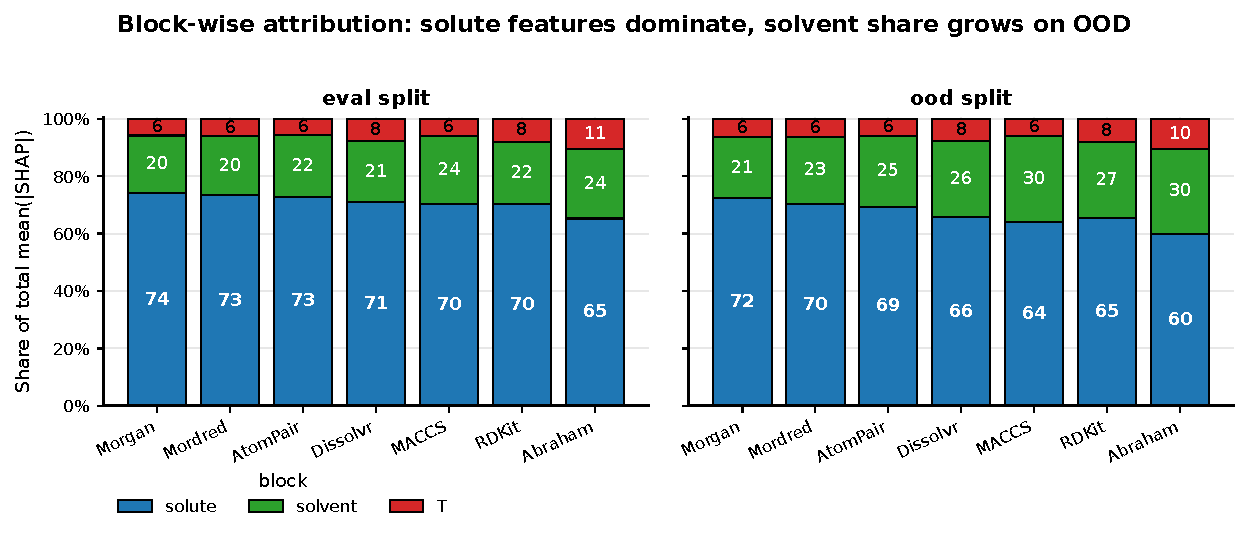
\includegraphics[width=\linewidth]{figures/fig1_blockwise.pdf}
\caption{\textbf{Block-wise SHAP attribution.}  Stacked bars show the
fraction of total mean(|SHAP|) coming from the solute, solvent, and
temperature blocks for each of the seven LightGBM\,$+$\,featurizer
runs, on \texttt{eval} (left) and \texttt{ood} (right).  The
\emph{solute} dominates universally (\numval{60}--\numval{74}\,\%) and
the share is remarkably stable across representations.  Going from
\texttt{eval} to \texttt{ood} consistently shifts mass from solute to
solvent (\(+3\)--\(+6\,\)pp): when the solvent set is unfamiliar the
model leans more on solvent features.}
\label{fig:interp_blockwise}
\end{figure}

Three observations stand out.

First, the solute carries roughly \numval{70}\,\% of the total
attribution mass on \texttt{eval} and the solvent only
\numval{20}\,\%, almost independently of representation.  This is
counter-intuitive given the SC$^{3}$ premise that solubility is a
function of the \emph{pair}, not of either component alone, and it
reframes what tabular models trained on \scthree{} are actually
optimising: most of the loss is reduced by knowing the solute, and
solvent identity is a comparatively modest correction term.

Second, the temperature block consumes \numval{6}--\numval{11}\,\% of
the attribution mass.  Abraham-only is the outlier (\numval{11}\,\% on
\texttt{eval}) because with only 6 chemistry features per molecule the
model has less to spend, so the four temperature features become
relatively more important.  This is an information-theoretic effect,
not a chemistry effect.

Third, every featurizer shifts \(\approx +3\)--\(+6\) percentage points
from solute to solvent when moving \texttt{eval}\(\to\)\texttt{ood}
(MACCS: \numval{24}\,\%\(\to\)\numval{30}\,\%;  Abraham:
\numval{24}\,\%\(\to\)\numval{30}\,\%).  This is exactly the behaviour
a well-generalising model should show: when the test solvents differ
from the training solvents, the model invests more attribution in the
solvent features it can still recognise.  Solvent identity is the
ground-truth nuisance variable; the model's response to OOD is to
lean on it harder.

% -----------------------------------------------------------------------------
\subsection{Top global features and the General Solubility Equation}
\label{sec:interp_global}

Drilling one level deeper, Figure~\ref{fig:interp_global_top} shows
the top-12 features for the three chemistry-readable representations
(RDKit, Dissolvr, Abraham-only).  We omit the fingerprint variants
because their top features are individual hashed bits without a
direct chemistry interpretation.

\begin{figure}[t]
\centering
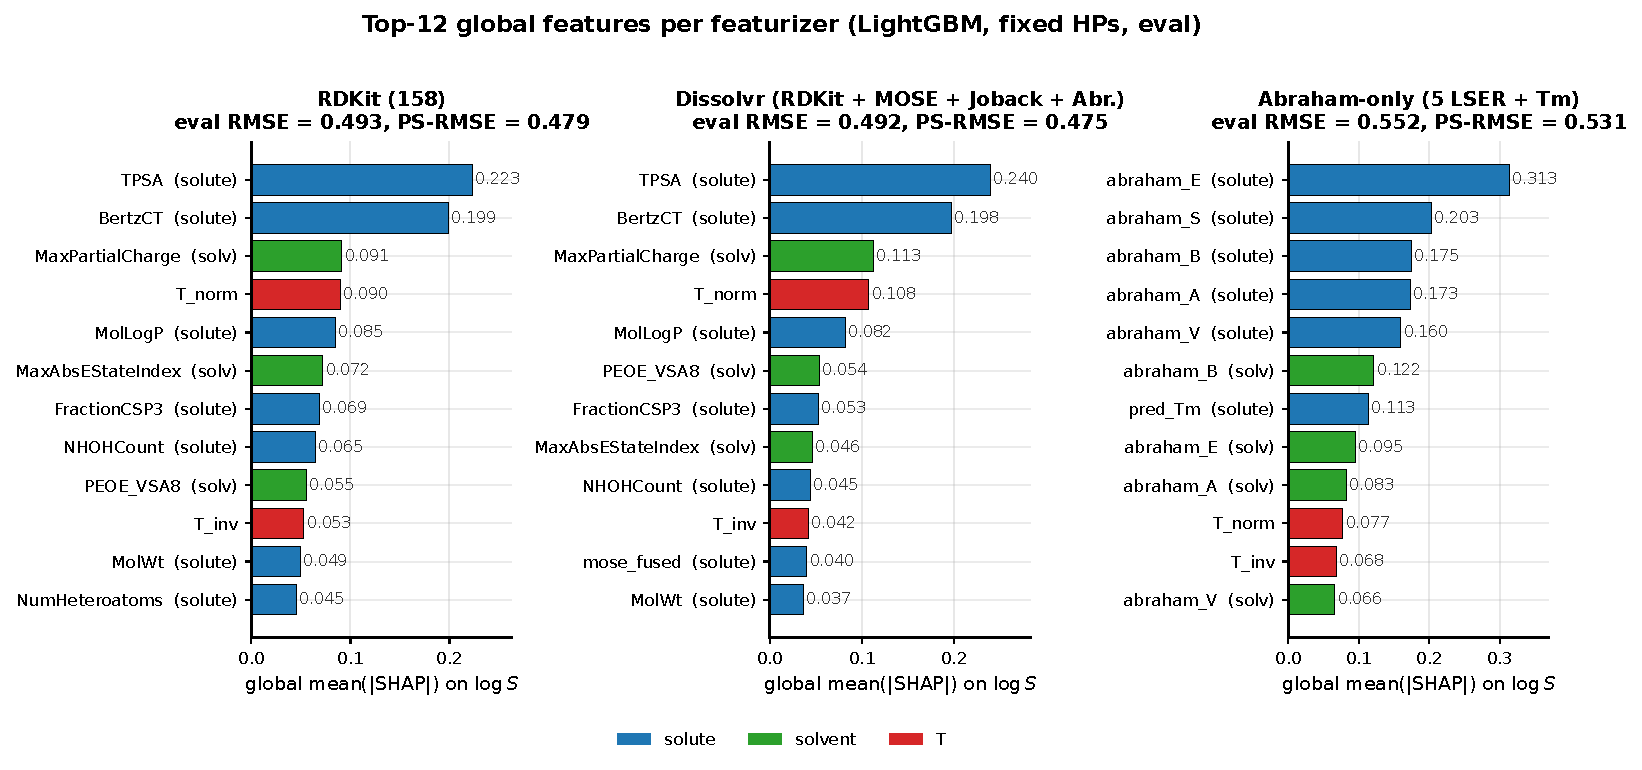
\includegraphics[width=\linewidth]{figures/fig2_global_top_features.pdf}
\caption{\textbf{Top-12 features per featurizer (LightGBM, eval).}
Bars are the global mean(|SHAP|) on \logS{}; colour encodes the
block (blue\,$=$\,solute, green\,$=$\,solvent, red\,$=$\,temperature).
On all three descriptor representations the top features are exactly
the axes of the General Solubility Equation: a polar surface area term
(\texttt{TPSA} / \texttt{TopoPSA(NO)}), a complexity term
(\texttt{BertzCT}), a logP term (\texttt{MolLogP}), a solvent
polarity proxy (\texttt{MaxPartialCharge}), and a temperature term
(\texttt{T\_norm}).  Abraham-only correctly recovers the canonical
LSER ranking $E > S \approx B \approx A > V$ on the solute side.}
\label{fig:interp_global_top}
\end{figure}

The headline result is that LightGBM, given no prior chemistry
knowledge, independently rediscovers \emph{the same axes} that
classical solubility equations were built around.  The Yalkowsky
General Solubility Equation~\cite{yalkowsky1980solubility} is
\(\logS \approx 0.5 - \log P - 0.01\,(T_m - 25)\), a linear function
of just two solute properties; SHAP says the LightGBM model is
fundamentally doing the same thing -- only with TPSA and BertzCT
included as additional polarity and complexity correction terms,
plus a temperature-from-data correction.

A quantitative aside: classical GSE puts the melting-point term
(\texttt{pred\_Tm}) at coefficient \(-0.01\) and gives it large
predictive weight.  In our SHAP ranking on Dissolvr (which contains
both \texttt{MolLogP} and the Joback \texttt{pred\_Tm} proxy),
\texttt{pred\_Tm} only reaches global mean(|SHAP|) \(\approx\)
\numval{0.029}, an order of magnitude below \texttt{TPSA}
(\numval{0.240}) and \texttt{BertzCT} (\numval{0.198}).  Our data
say polarity dominates crystal packing for \scthree{}-style liquid
solubility predictions much more than Yalkowsky's coefficients
suggest.

The Abraham-only panel is the cleanest test of the LSER analogue:
running LightGBM on just six features per molecule
(\(A, B, S, E, V, T_m\)) gives a top ranking of
\(E_{\mathrm{solute}} > S_{\mathrm{solute}} > B_{\mathrm{solute}}
\approx A_{\mathrm{solute}} > V_{\mathrm{solute}}\), matching the
canonical LSER coefficient ordering for aqueous and organic
solubility~\cite{abraham1993scales}.  The first solvent-side feature
is \(B_{\mathrm{solv}}\) (H-bond basicity), at rank 6, which is the
correct LSER axis to rank first on the solvent side as well.

The magnitude plots above answer the question ``what matters?''
but not the complementary question ``in which direction?''  To get a
directional readout we compute, for every feature, Spearman's
\(\rho\) between the raw feature value \(x_j\) and its SHAP
contribution \(\phi_j(x)\) over the \texttt{eval} split.  Positive
\(\rho\) means larger feature values tend to push predicted \logS{}
up; negative \(\rho\) means larger values tend to push it down.  This
is not a causal derivative -- it is the model's learned association
after all tree interactions -- but it makes the chemistry much more
actionable.

\begin{figure}[t]
\centering
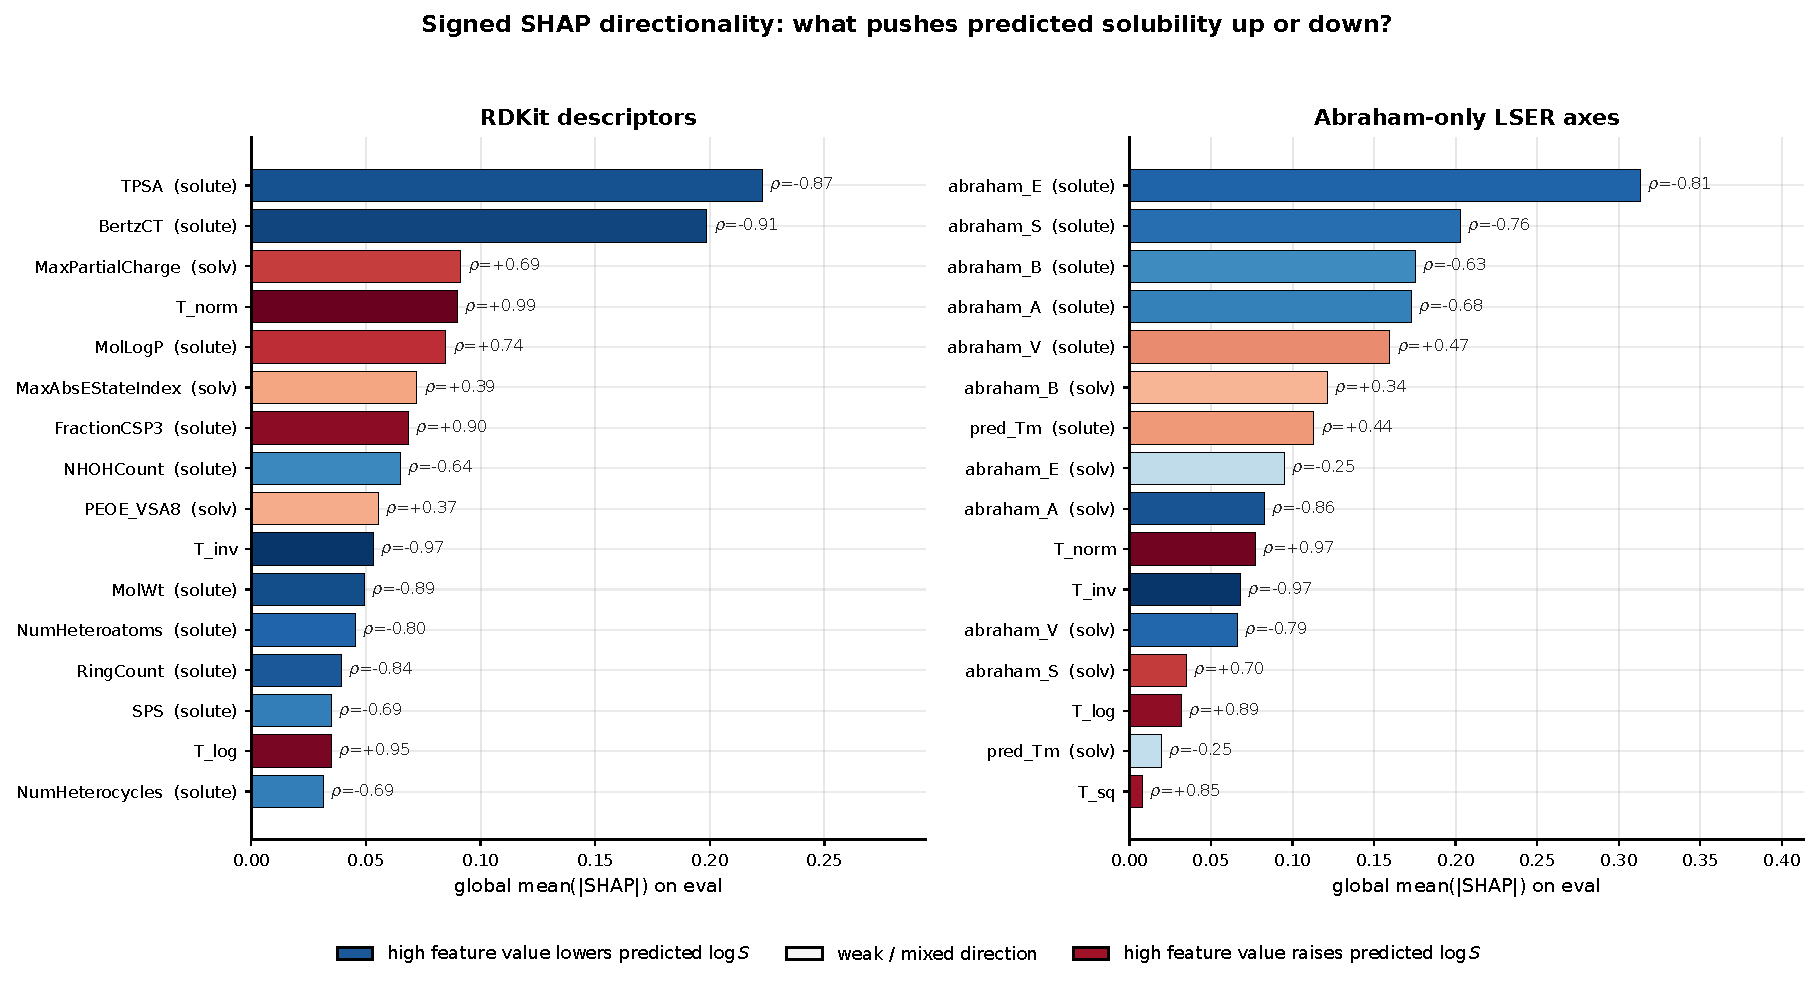
\includegraphics[width=\linewidth]{figures/fig8_signed_shap.pdf}
\caption{\textbf{Signed SHAP directionality.}  Bar length is the usual
global mean(|SHAP|), so the ranking is unchanged from
Figure~\ref{fig:interp_global_top}.  Bar colour and the printed
Spearman \(\rho\) show direction: blue features have high values that
lower predicted \logS{}, red features have high values that raise
predicted \logS{}.  The descriptor panel says the strongest solute
features -- \texttt{TPSA}, \texttt{BertzCT}, \texttt{MolWt},
\texttt{RingCount}, heteroatom counts -- mostly push predictions
down when large, while temperature and solvent partial-charge features
push predictions up.  The Abraham-only panel makes the LSER story
explicit: solute \(E,S,B,A\) lower predicted solubility when large,
whereas increasing temperature raises it.}
\label{fig:interp_signed_shap}
\end{figure}

Two details are worth noting.  First, high \texttt{T\_norm} has
\(\rho\approx +0.99\) and high \texttt{T\_inv} has
\(\rho\approx -0.97\), exactly the expected thermodynamic monotonicity:
the model has learned that higher temperature usually increases
solubility.  Second, the solute descriptor directions are not simply
``more polar means more soluble''.  On the multi-solvent aggregate,
large TPSA and large Abraham \(E/S/B/A\) values tend to lower the
global prediction.  This is not contradictory to aqueous intuition:
the dataset is dominated by organic solvents, and the signed SHAP
score is a conditional association in the fitted model, not a
one-solvent causal law.  The per-solvent analysis below is therefore
essential; the global signed plot is a direction-of-effect summary,
not a universal chemical rule.

% -----------------------------------------------------------------------------
\subsection{Per-solvent profiles}
\label{sec:interp_per_solvent}

We can also slice the SHAP attribution by solvent.  For each of the
top-25 in-distribution solvents (the \texttt{eval} solvent set), we
restrict to the rows where that solvent is the medium and compute
mean(|SHAP|) per feature.  Figure~\ref{fig:interp_per_solvent_heatmap}
shows the result for Dissolvr; each column sums to one, so the
heatmap reads as ``which feature does the model lean on, given this
solvent''.

\begin{figure}[t]
\centering
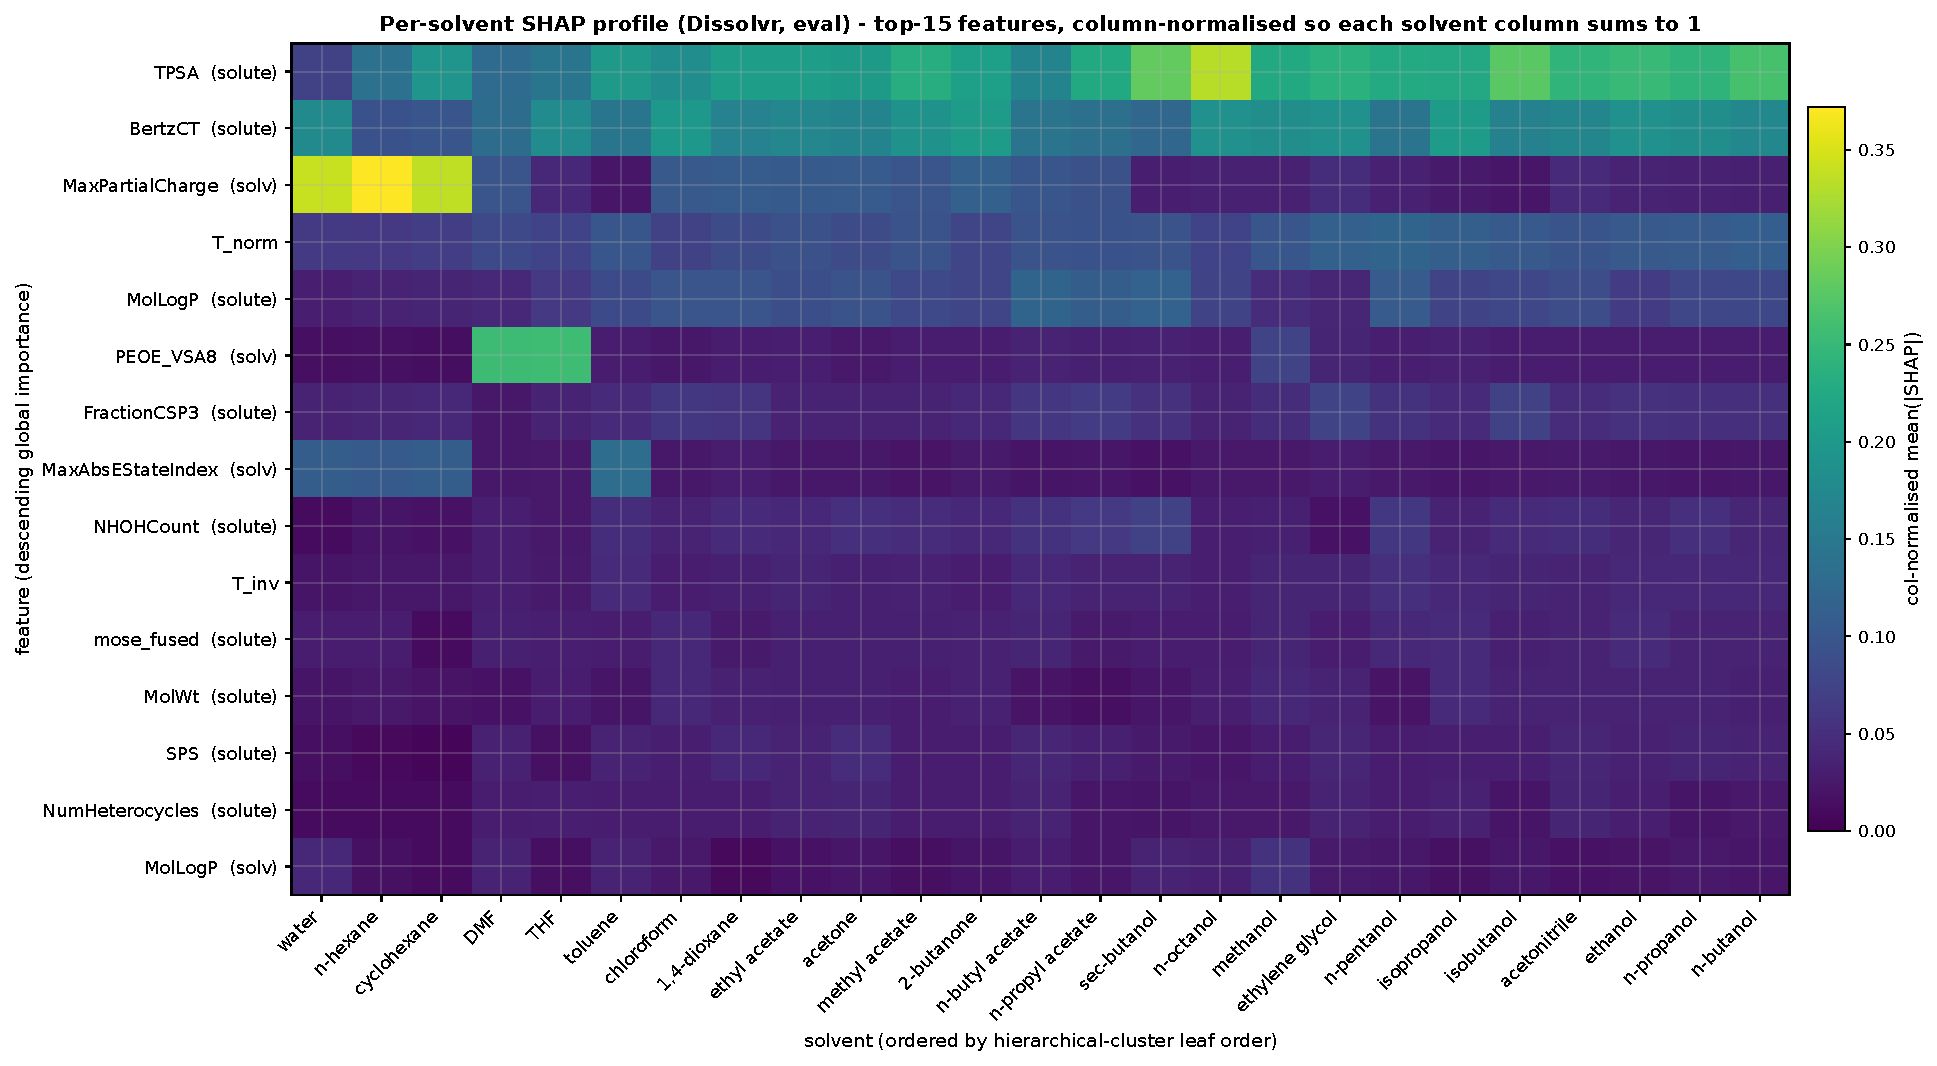
\includegraphics[width=\linewidth]{figures/fig3_per_solvent_heatmap.pdf}
\caption{\textbf{Per-solvent SHAP profile (Dissolvr, eval).}  Rows are
the top-15 globally-important features (descending); columns are the
25 \texttt{eval} solvents, ordered by hierarchical clustering on the
column vectors.  Cells are column-normalised mean(|SHAP|), so darker
\(=\) less important relative to the rest of that solvent's profile.
Two qualitative patterns are visible: (i) for typical organic
solvents the model relies on \texttt{TPSA} and \texttt{BertzCT} of
the \emph{solute}; (ii) for the extreme solvents (water, n-hexane,
cyclohexane) it switches to \texttt{MaxPartialCharge} and
\texttt{MaxAbsEStateIndex} of the \emph{solvent}.  A third specialised
pattern shows up for DMF and THF, where \texttt{PEOE\_VSA8} of the
solvent dominates.}
\label{fig:interp_per_solvent_heatmap}
\end{figure}

Three distinct per-solvent regimes appear: ``alcohols and esters''
(the broad band on the right where \texttt{TPSA(solute)} dominates),
``alkanes \(+\) water'' (the leftmost columns where
\texttt{MaxPartialCharge(solv)} dominates), and ``aprotic-aromatic''
(DMF, THF, with \texttt{PEOE\_VSA8(solv)} dominant).  Per-solvent
top-3 feature lists are summarised in Table~\ref{tab:interp_anchor_solvents}
for the five anchor solvents most often used as references in the
solubility literature.

\begin{table}[t]
\centering\small
\caption{Per-solvent top-3 SHAP features (RDKit, eval).  ``solv''
prefix denotes solvent-side features; otherwise the feature is on the
solute.  N is the number of \texttt{eval} rows for that solvent.}
\label{tab:interp_anchor_solvents}
\renewcommand{\arraystretch}{1.10}
\begin{tabular}{@{}llrl@{}}
\toprule
Solvent      & N    & rank 1 (mean\,|SHAP|)            & ranks 2-3 \\
\midrule
\textbf{water}        & \numval{397} & \texttt{solv\_MaxPartialCharge}  (\numval{0.50}) & \texttt{solv\_MaxAbsEStateIndex}, \texttt{solute\_BertzCT} \\
\textbf{n-hexane}     & \numval{120} & \texttt{solv\_MaxPartialCharge}  (\numval{0.53}) & \texttt{solv\_MaxAbsEStateIndex}, \texttt{solute\_TPSA} \\
\textbf{DMF}          & \numval{263} & \texttt{solv\_PEOE\_VSA8}        (\numval{0.34}) & \texttt{solute\_BertzCT}, \texttt{solute\_TPSA} \\
\textbf{ethanol}      & \numval{782} & \texttt{solute\_TPSA}             (\numval{0.24}) & \texttt{solute\_BertzCT}, \texttt{T\_norm} \\
\textbf{methanol}     & \numval{594} & \texttt{solute\_TPSA}             (\numval{0.23}) & \texttt{solute\_BertzCT}, \texttt{solv\_PEOE\_VSA8} \\
\textbf{toluene}      & \numval{222} & \texttt{solute\_TPSA}             (\numval{0.24}) & \texttt{solv\_MaxAbsEStateIndex}, \texttt{solute\_BertzCT} \\
\textbf{chloroform}   & \numval{ 80} & \texttt{solute\_BertzCT}          (\numval{0.24}) & \texttt{solute\_TPSA}, \texttt{solute\_MolLogP} \\
\textbf{acetonitrile} & \numval{456} & \texttt{solute\_TPSA}             (\numval{0.24}) & \texttt{solute\_BertzCT}, \texttt{solute\_MolLogP} \\
\bottomrule
\end{tabular}
\end{table}

The pattern is consistent: in 22 of 25 \texttt{eval} solvents two of
the top-3 features are solute features.  Only for water and the
two alkanes (n-hexane, cyclohexane) do solvent-side features
take the top-2 slots.  This suggests the model uses solvent-side
features as a coarse \emph{gate}: ``decide what kind of solvent we
are in, then evaluate the solute against that gate's specialised
sub-model''.  The number of distinct gates is small -- about four,
matching the four solvent families recovered by the clustering analysis
of Section~\ref{sec:interp_clustering}.

% -----------------------------------------------------------------------------
\subsection{Solvents the model treats similarly}
\label{sec:interp_clustering}

Each solvent's SHAP profile vector (Section~\ref{sec:interp_per_solvent})
defines a per-solvent fingerprint in feature-importance space.
Two solvents with similar fingerprints are, by construction, treated
similarly by the model: it weights the same features when predicting
solubility in either.  We compute the cosine similarity between every
pair of solvent fingerprints (using the top-50 globally-important
features as the vector basis) and run hierarchical clustering with
average linkage.

\begin{figure}[t]
\centering
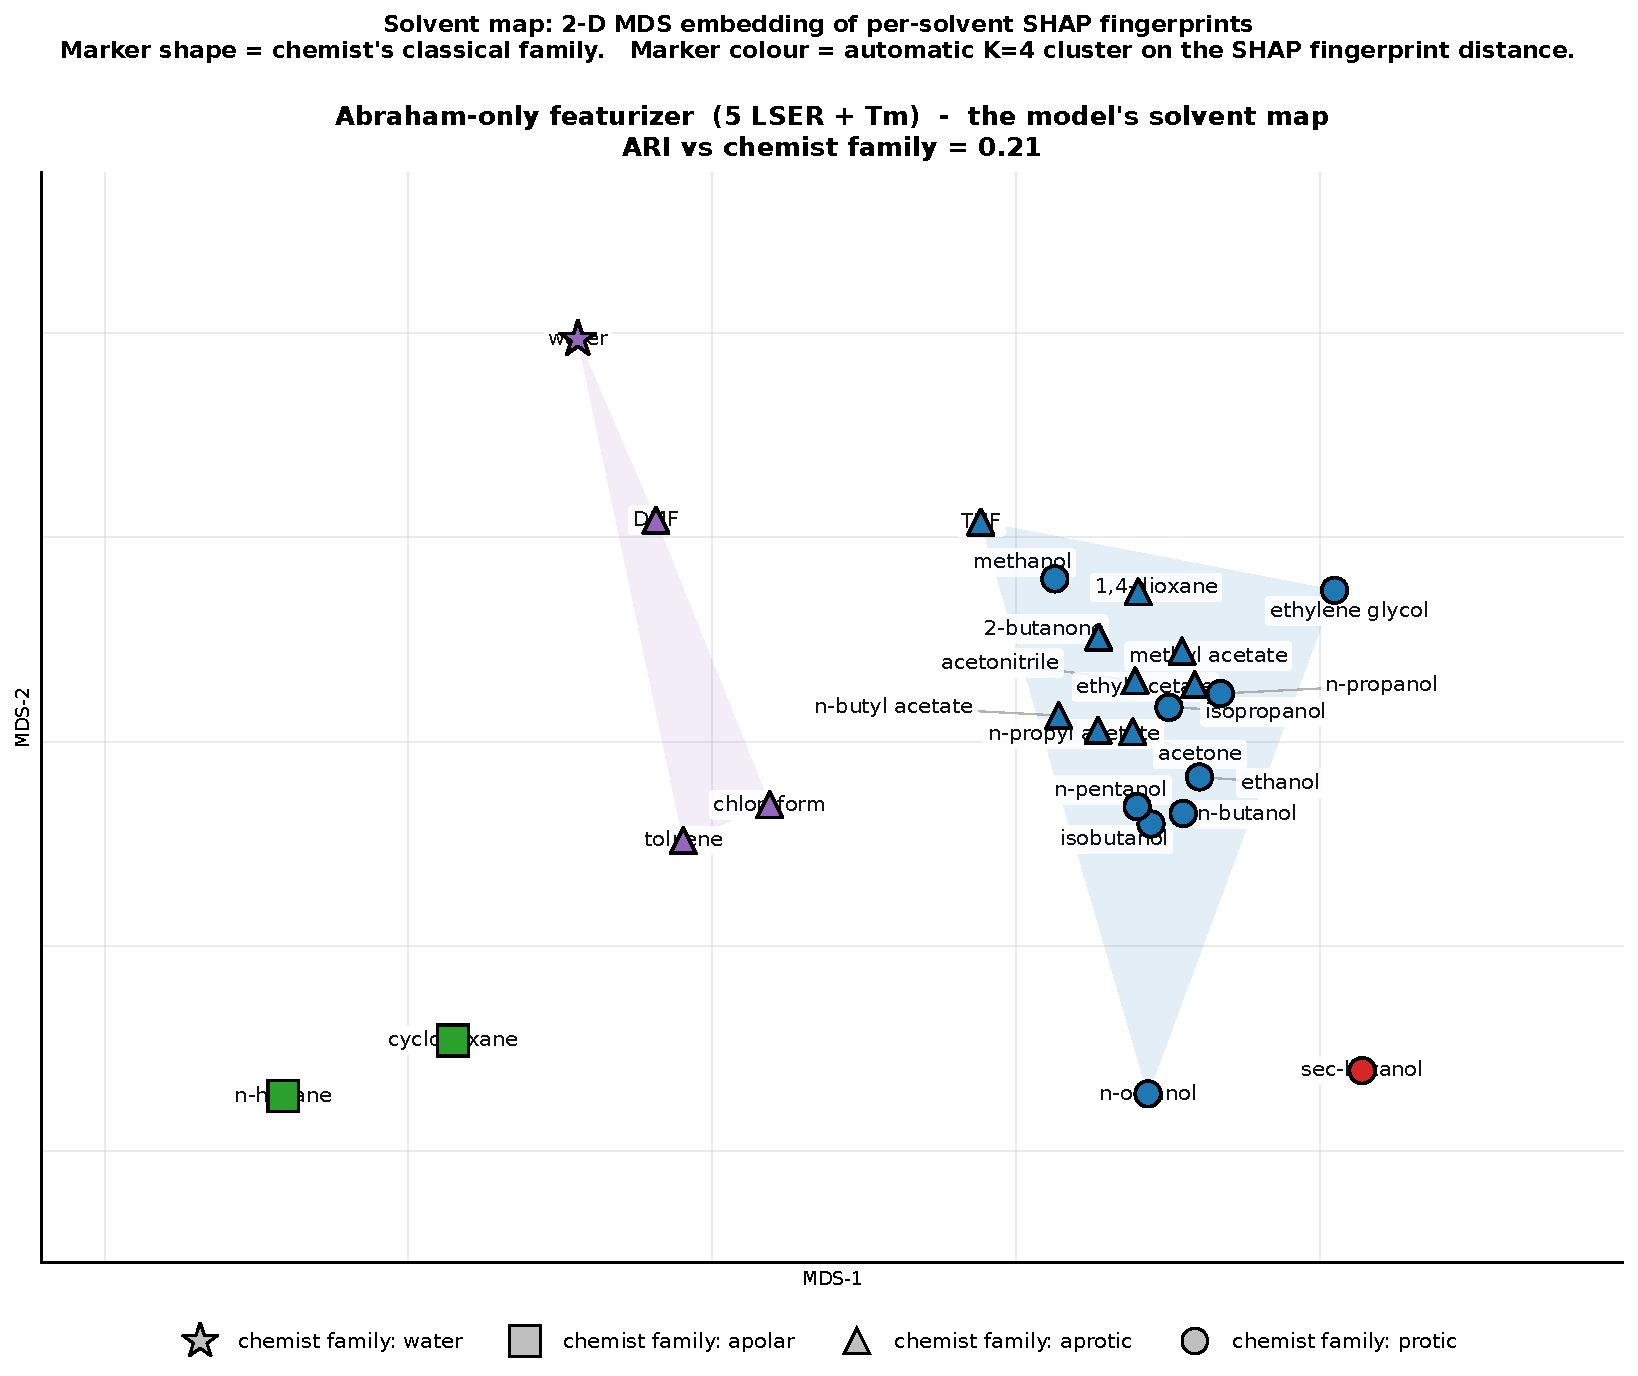
\includegraphics[width=\linewidth]{figures/fig4c_solvent_map_hero.pdf}
\caption{\textbf{Solvent map under the Abraham-only featurizer.}
Each point is one of the 25 \texttt{eval} solvents at its 2-D MDS
coordinates derived from the per-solvent SHAP fingerprint distance
\(1 - \cos(\cdot)\).  \textbf{Marker shape} encodes the chemist's
classical Snyder family (\(\star\)~water, \(\blacksquare\)~apolar
alkane, \(\blacktriangle\)~aprotic, \(\bullet\)~protic alcohol).
\textbf{Marker colour} encodes the model's automatic cluster (K=4
average-linkage hierarchical, on the same distance).  Same colour
\(=\) the model treats those solvents the same way; same shape
\(=\) chemists treat them the same way.  Disagreements -- such as
the model placing water in the same purple cluster as DMF /
chloroform / toluene -- are visually obvious.  ARI vs the chemist
labelling \(=\) \numval{0.21}.}
\label{fig:interp_solvent_map}
\end{figure}

\begin{figure}[t]
\centering
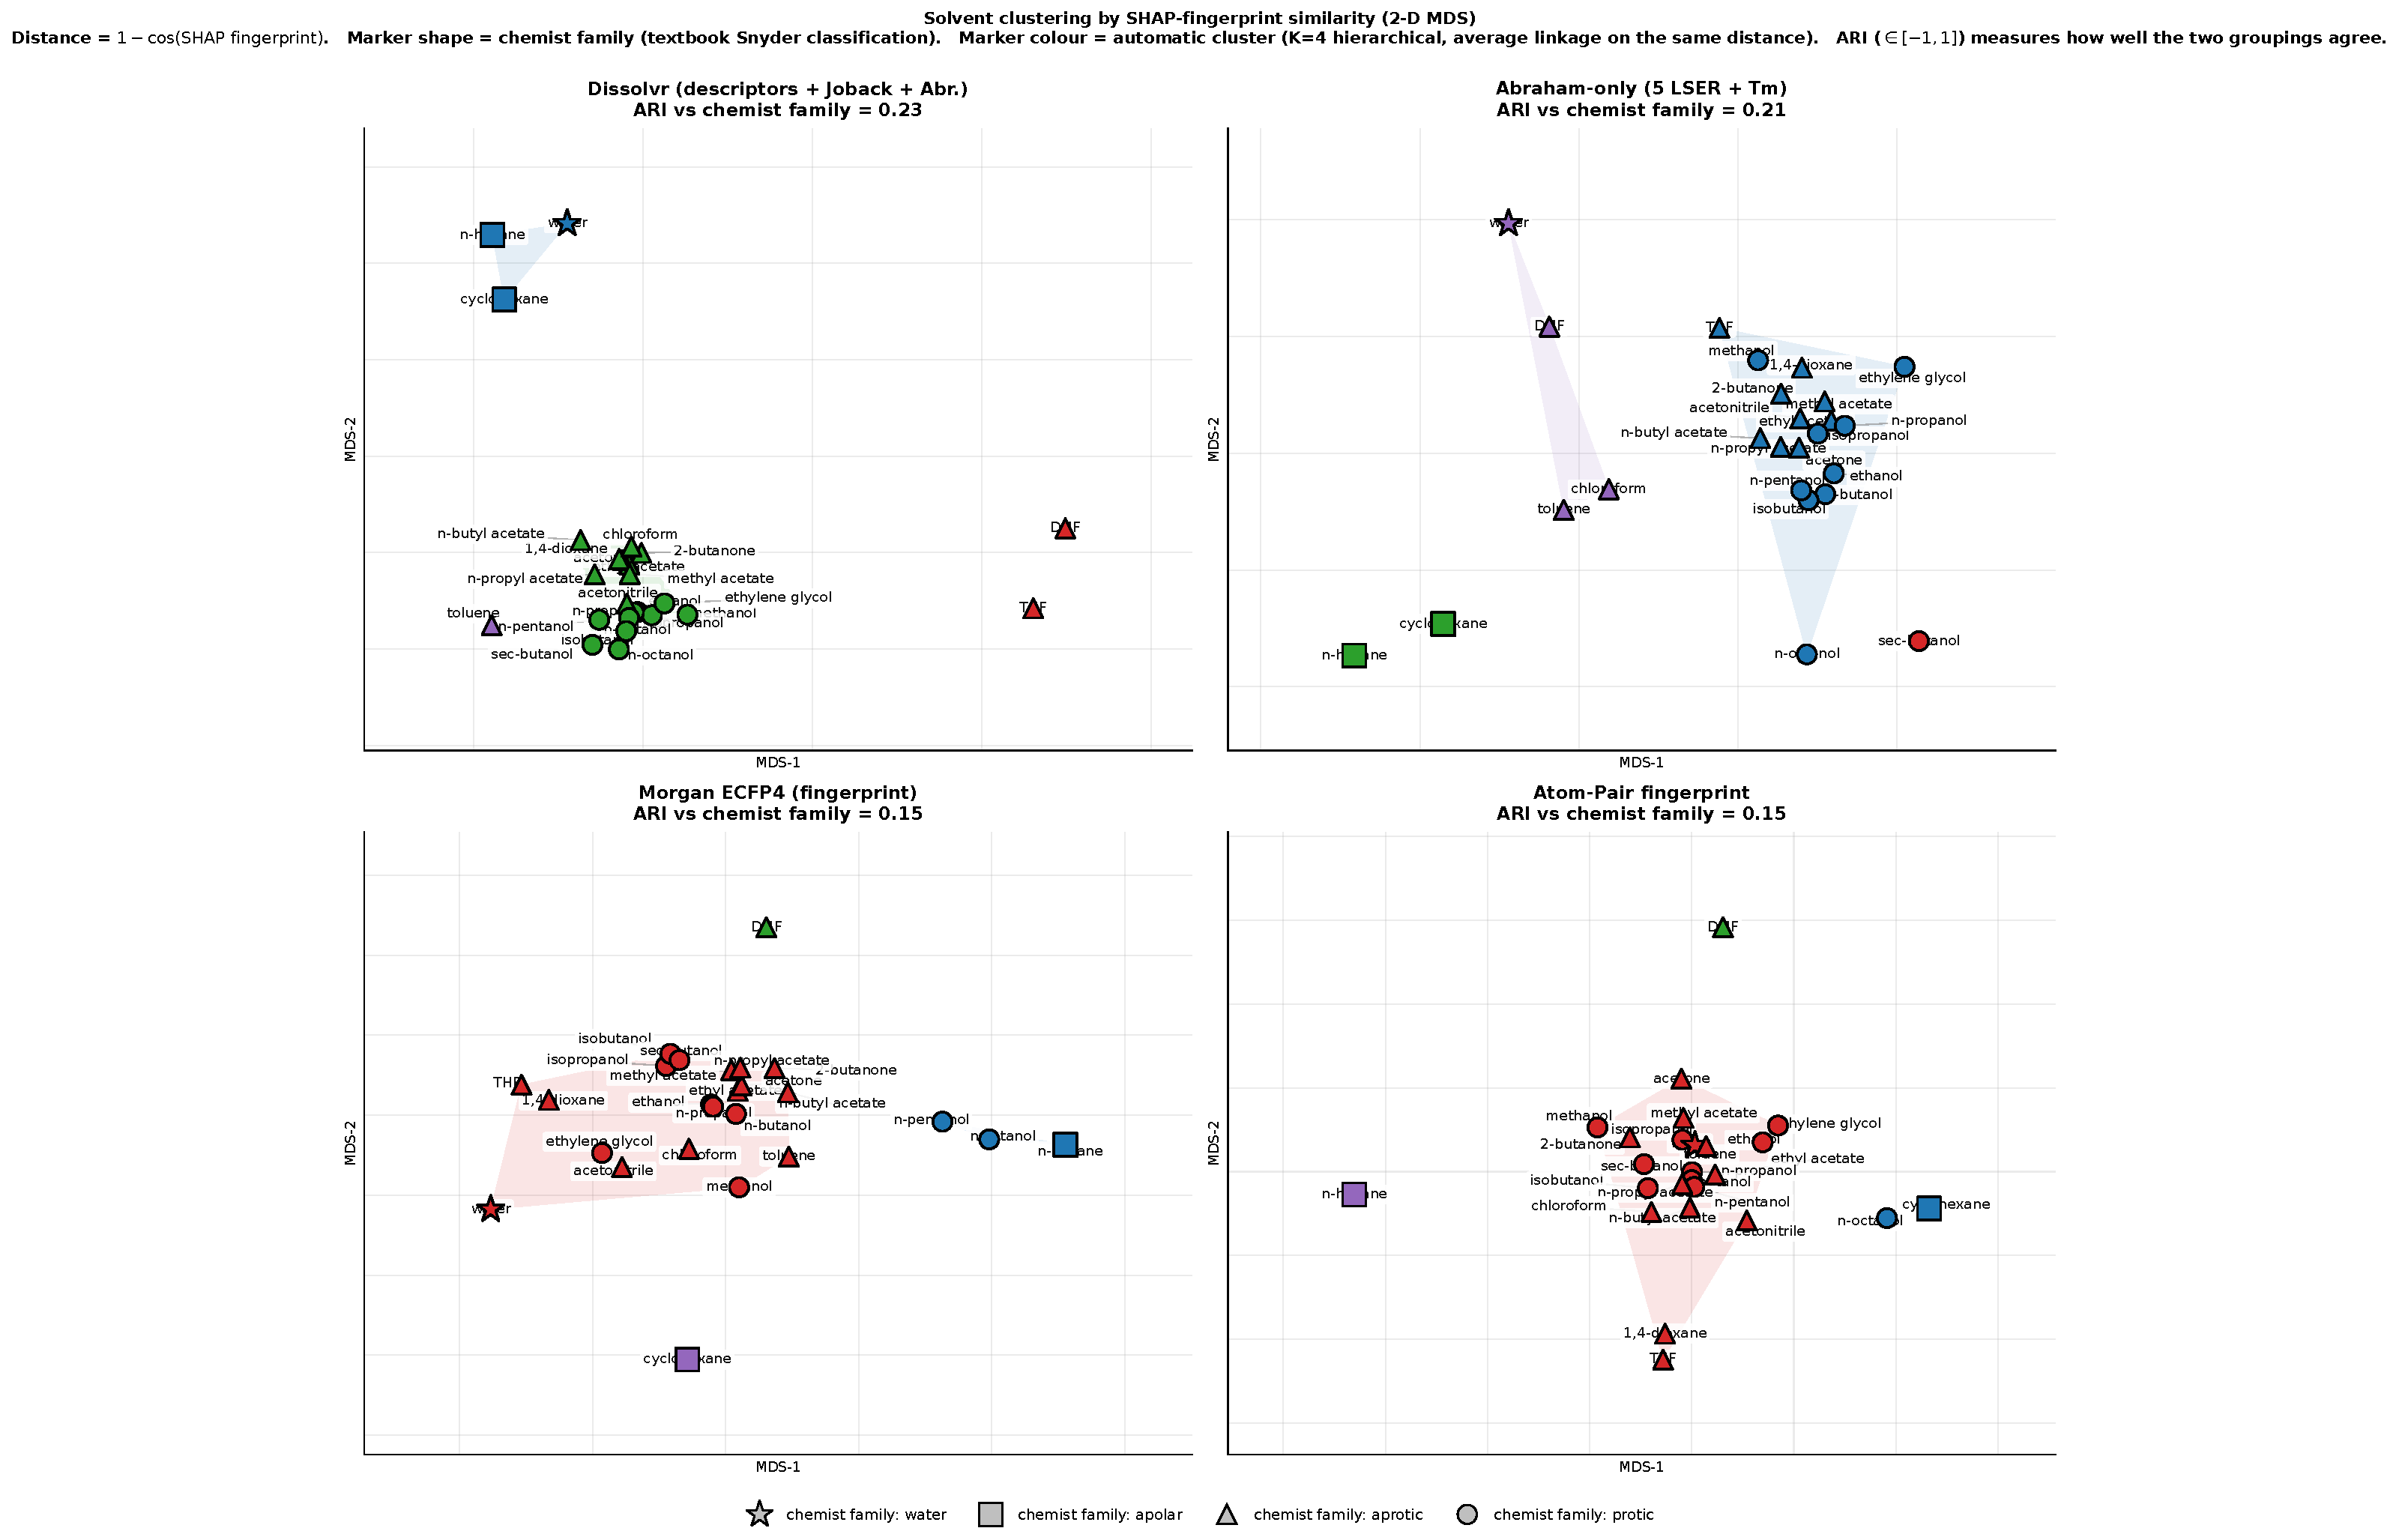
\includegraphics[width=\linewidth]{figures/fig4b_solvent_clusters_2d.pdf}
\caption{\textbf{Solvent maps across four featurizers.}  Same MDS-on-SHAP
construction as Figure~\ref{fig:interp_solvent_map} but with one
panel per featurizer.  Top row (\textit{descriptor / Abraham}) cleanly
separates water, alkanes, the aprotic-aromatic group (DMF / THF /
chloroform / toluene), and a large alcohol-and-ester cluster.
Bottom row (\textit{circular fingerprints}) is structurally driven --
it isolates DMF and cyclohexane as singletons, places n-hexane next
to long-chain alcohols, and dumps everything else into one mass --
a chemistry-blind grouping.  ARI scores quantify the agreement gap
(\numval{0.21}--\numval{0.23} for descriptors vs.\ \numval{0.15} for
fingerprints).}
\label{fig:interp_dendrograms}
\end{figure}

Figure~\ref{fig:interp_solvent_map} shows the headline result for
Abraham-only and Figure~\ref{fig:interp_dendrograms} compares all
four featurizers in the same coordinate system.

On the descriptor representations the model partitions the solvents
into four chemistry-readable groups: water, alkanes, an
aprotic-aromatic cluster (DMF, THF, chloroform, toluene), and one
large band that contains the alcohols, esters, ketones, ethers,
acetonitrile, and dioxane.  The first three groups match the chemist's
families one-to-one; the fourth is a genuine model artefact -- under
the descriptor view those 16 solvents really do have nearly identical
SHAP fingerprints, because the model's attribution mass on solvent
features is small (\(\sim\)\numval{20}\,\%, Section~\ref{sec:interp_blockwise})
and the residual variance is dominated by the solute.  In other words,
the model itself reports that those 16 solvents are interchangeable
to within its own resolution.

The fingerprint-based maps tell a strikingly different story.  Morgan
ECFP4 isolates DMF, cyclohexane, and water as solitary outliers and
groups n-hexane with n-pentanol and n-octanol -- chemically
incoherent, because those latter two are protic alcohols of distinct
functional class.  This is structural similarity (long carbon chains
share Morgan bits) masquerading as chemical similarity.  The Atom-Pair
fingerprint behaves the same way.  The Adjusted Rand Index quantifies
the gap: \numval{0.21}--\numval{0.23} for the descriptor / Abraham
maps vs.\ \numval{0.15} for the fingerprints.

This is the mechanistic complement of the Representation ablation's
RMSE story.  The Representation ablation showed circular fingerprints
trail descriptors by \(\approx\) \numval{0.15} \RMSE{} on
\texttt{ood} and \texttt{sc3\_gold}; here we see \emph{why} -- the
fingerprint model has no internal representation under which water
behaves differently from a long-chain alcohol -- and so it cannot
specialise its prediction the way a descriptor model can.

A complementary hierarchical-clustering dendrogram view of the same
distance matrix is included in
\path{vansh/Ablations/Interpretability/paper_figures/fig4_solvent_dendrograms.pdf};
the two visualisations are mathematically equivalent (same distance,
same linkage; only the 2-D projection vs.\ tree drawing differs).

% -----------------------------------------------------------------------------
\subsection{Abraham/LSER axes per solvent}
\label{sec:interp_abraham}

The 6-feature Abraham-only representation makes the solvatochemistry
unusually transparent: every feature has a textbook physical meaning
($A$ = H-bond acidity, $B$ = H-bond basicity, $S$ = dipolarity /
polarisability, $E$ = excess molar refractivity, $V$ = molar volume,
$T_m$ = melting-point proxy).  Figure~\ref{fig:interp_abraham} shows
the per-solvent breakdown of mean(|SHAP|) along each axis,
side-by-side for the solvent block (left) and the solute block
(right).

\begin{figure}[t]
\centering
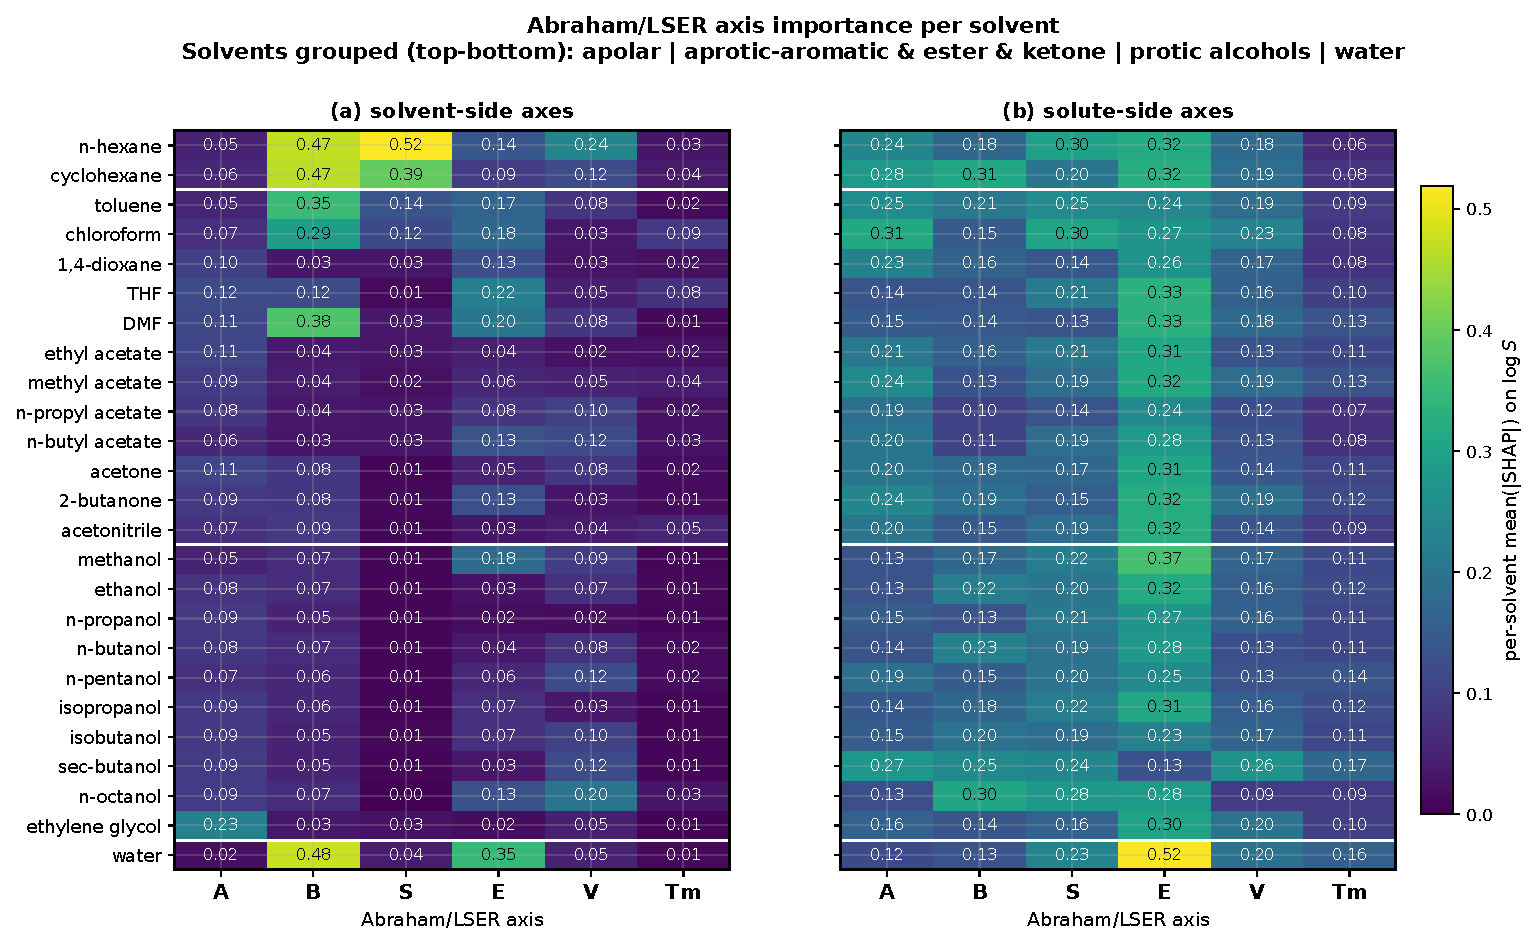
\includegraphics[width=\linewidth]{figures/fig5_abraham_lser.pdf}
\caption{\textbf{Abraham/LSER axis importance per solvent.}  Rows are
solvents grouped (top-bottom) into apolar, aprotic-aromatic
\(+\)~ester~/~ketone, protic alcohols, and water.  Columns are the
six Abraham/LSER axes.  Cells are mean(|SHAP|) for that
(side, solvent, axis) cell on \texttt{eval}.  The panel reads as a
literal LSER table: alkanes have very large $B$ and $S$ on the
solvent side (the model uses the absence of those features to
identify the medium), water has a large solvent-side $E$ \emph{and}
the largest solute-side $E$ in the dataset, and DMF/toluene foreground
solvent-side $B$.}
\label{fig:interp_abraham}
\end{figure}

Several known-correct chemistry signals appear unprompted.  On the
solvent side, the \(B\) axis (H-bond basicity) is the dominant
feature for n-hexane, cyclohexane, water, DMF, and toluene -- exactly
the solvents whose \(B\) value is unusual (very low for alkanes,
very high for water/DMF, intermediate-aromatic for toluene).  On the
solute side, the \(E\) axis (excess molar refractivity / aromaticity
proxy) dominates everywhere, peaking sharply at solvent~$=$~water
(\numval{0.52}) -- which matches the well-known dependence of
aqueous solubility on solute aromaticity.  The model has independently
located the LSER axes that need to be high-leverage for predicting
solubility in each solvent class.

% -----------------------------------------------------------------------------
\subsection{Pairwise interactions}
\label{sec:interp_interactions}

So far every analysis has been an additive (main-effect) decomposition
of the predictions.  Tree-SHAP also defines exact \emph{interaction}
values $\Phi_{ij}$ that tell us how much of the prediction comes from
the joint use of features $i$ and $j$, after subtracting the main
effects.  Figure~\ref{fig:interp_interactions} shows the top-15
interaction pairs for Abraham-only (left, exact, \numval{1500}-row
\texttt{eval} sample) and RDKit (right, exact, \numval{200}-row
sample with \texttt{tree\_limit}=\numval{150} to keep compute
tractable).

\begin{figure}[t]
\centering
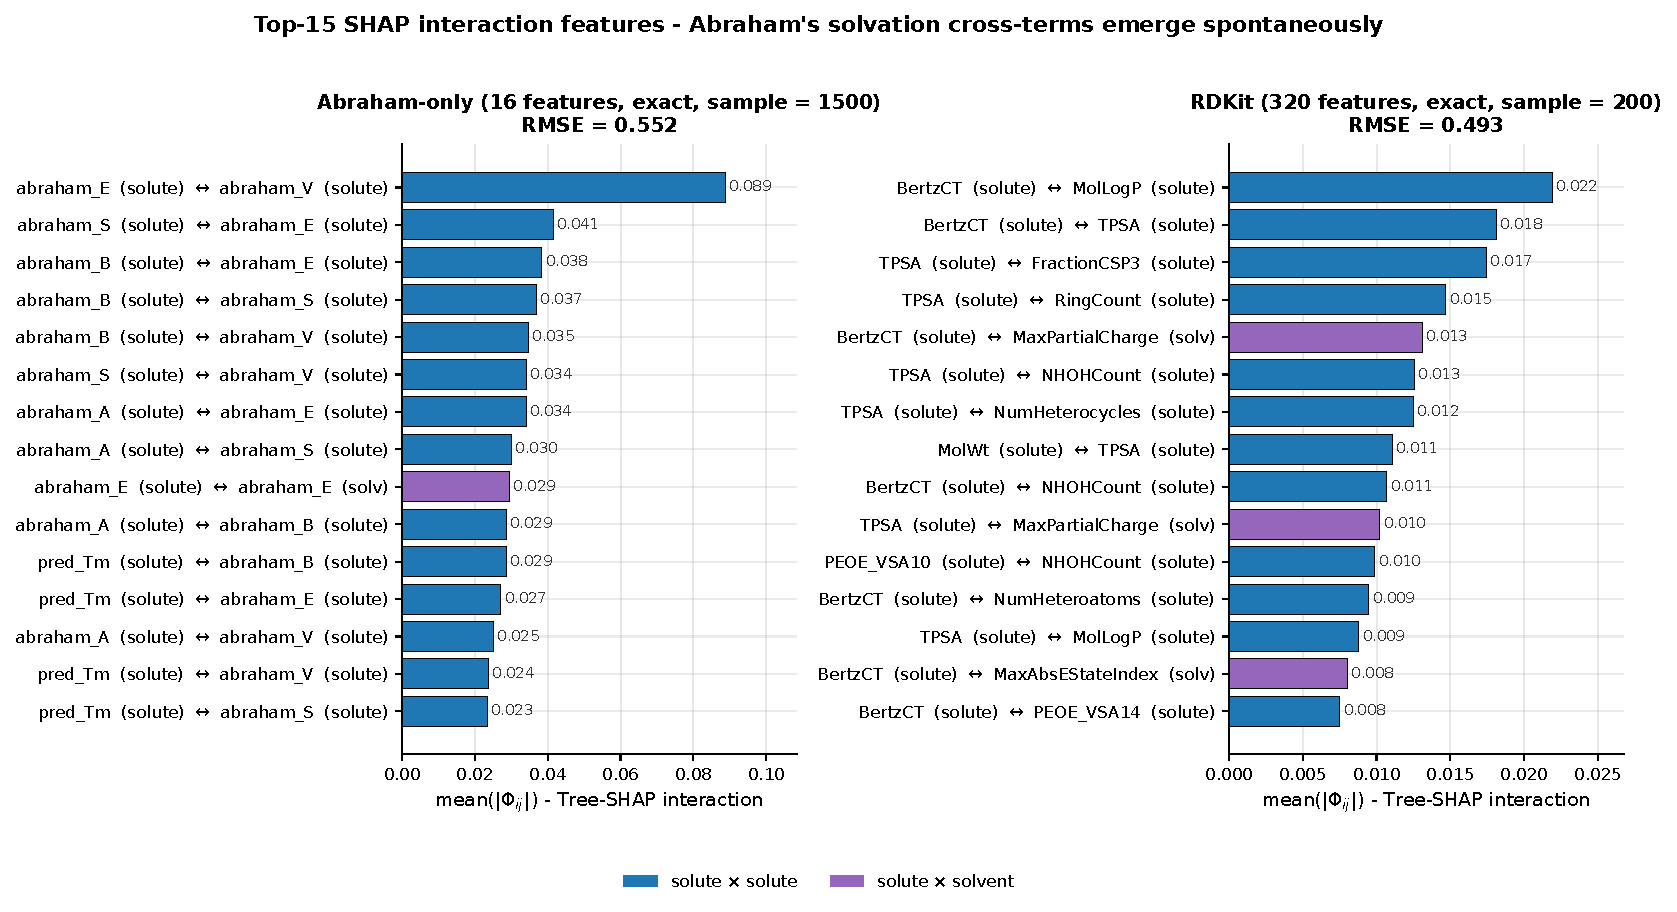
\includegraphics[width=\linewidth]{figures/fig6_interactions.pdf}
\caption{\textbf{Top SHAP interaction features.}  Bars are mean(|$\Phi_{ij}$|)
on \texttt{eval}; colour encodes the block-pair (solute$\times$solute,
solute$\times$solvent, etc.).  On Abraham-only, the top-8 pairs are
exclusively within the solute LSER axes (textbook within-molecule
solvation coupling); cross-block solute$\times$solvent pairs appear
from rank 9 onward and are matched-axis ($E\!\times\!E$,
$A\!\times\!A$, $E\!\times\!B$) -- the off-diagonal LSER cross-terms.
On RDKit, the top-4 pairs are within the GSE axes
(\texttt{BertzCT}\(\times\)\texttt{MolLogP}, etc.); the largest
cross-block interaction is \texttt{BertzCT(solute)}\(\times\)
\texttt{MaxPartialCharge(solv)}, the discrete analogue of a
partition coefficient term.}
\label{fig:interp_interactions}
\end{figure}

The Abraham-only panel reproduces the structure of Abraham's
solvation equation almost exactly.  The top interaction
($E_{\mathrm{solute}}\!\times\!V_{\mathrm{solute}}$, mean(|$\Phi$|)
= \numval{0.089}) is the same coupling the LSER equation writes as
$v\,V + e\,E$ -- cavity-formation cost coupled with the dispersion
term.  Pairs 2-8 are all other within-LSER couplings ($S\!\times\!E$,
$B\!\times\!E$, $B\!\times\!S$, etc.).  Cross-block (solute$\times$solvent)
matched-axis interactions appear from rank 9 onward
($E_{\mathrm{solute}}\!\times\!E_{\mathrm{solv}}$,
$A_{\mathrm{solute}}\!\times\!A_{\mathrm{solv}}$),
which is exactly the off-diagonal structure that LSER's
$\sum_k r_k\,k_{\mathrm{solute}}\,k_{\mathrm{solv}}$ cross-term
predicts.  No solvent-T or T-T interactions appear in the top 20:
temperature enters the model essentially additively.

The RDKit panel is the descriptor analogue.  The top four
interactions are all solute-side and span the GSE axes
(\texttt{BertzCT}\(\times\)\texttt{MolLogP},
\texttt{BertzCT}\(\times\)\texttt{TPSA},
\texttt{TPSA}\(\times\)\texttt{FractionCSP3},
\texttt{TPSA}\(\times\)\texttt{RingCount}).  The largest cross-block
pair is \texttt{BertzCT(solute)}\(\times\)\texttt{MaxPartialCharge(solv)}
at rank 5: the model gates the effect of solute complexity on
solubility by how polar the solvent is.  This is the only mechanism
by which a tabular tree model can express something resembling a
partition-coefficient (\(\log K_{ow}\)) term, and SHAP shows it doing
so explicitly.

% -----------------------------------------------------------------------------
\subsection{Graph-based interpretation: GCN}
\label{sec:interp_gcn}

The SHAP analysis above is unique to tree-based models.  For the
dual-encoder GCN we use occlusion attribution: for each
(\textit{solute}, \textit{solvent}, \(T\)) triple in a sample of
\numval{5000} \texttt{eval} rows, we compute the model's prediction
once with the full graph and once with each solute atom's node
features set to zero, recording the absolute change \(|\Delta\,\logS|\).
This gives \numval{85062} per-atom attribution scores, which we
aggregate two ways: by atom type (Figure~\ref{fig:interp_gcn}a) and
by BRICS fragment containing the atom (Figure~\ref{fig:interp_gcn}b).

\begin{figure}[t]
\centering
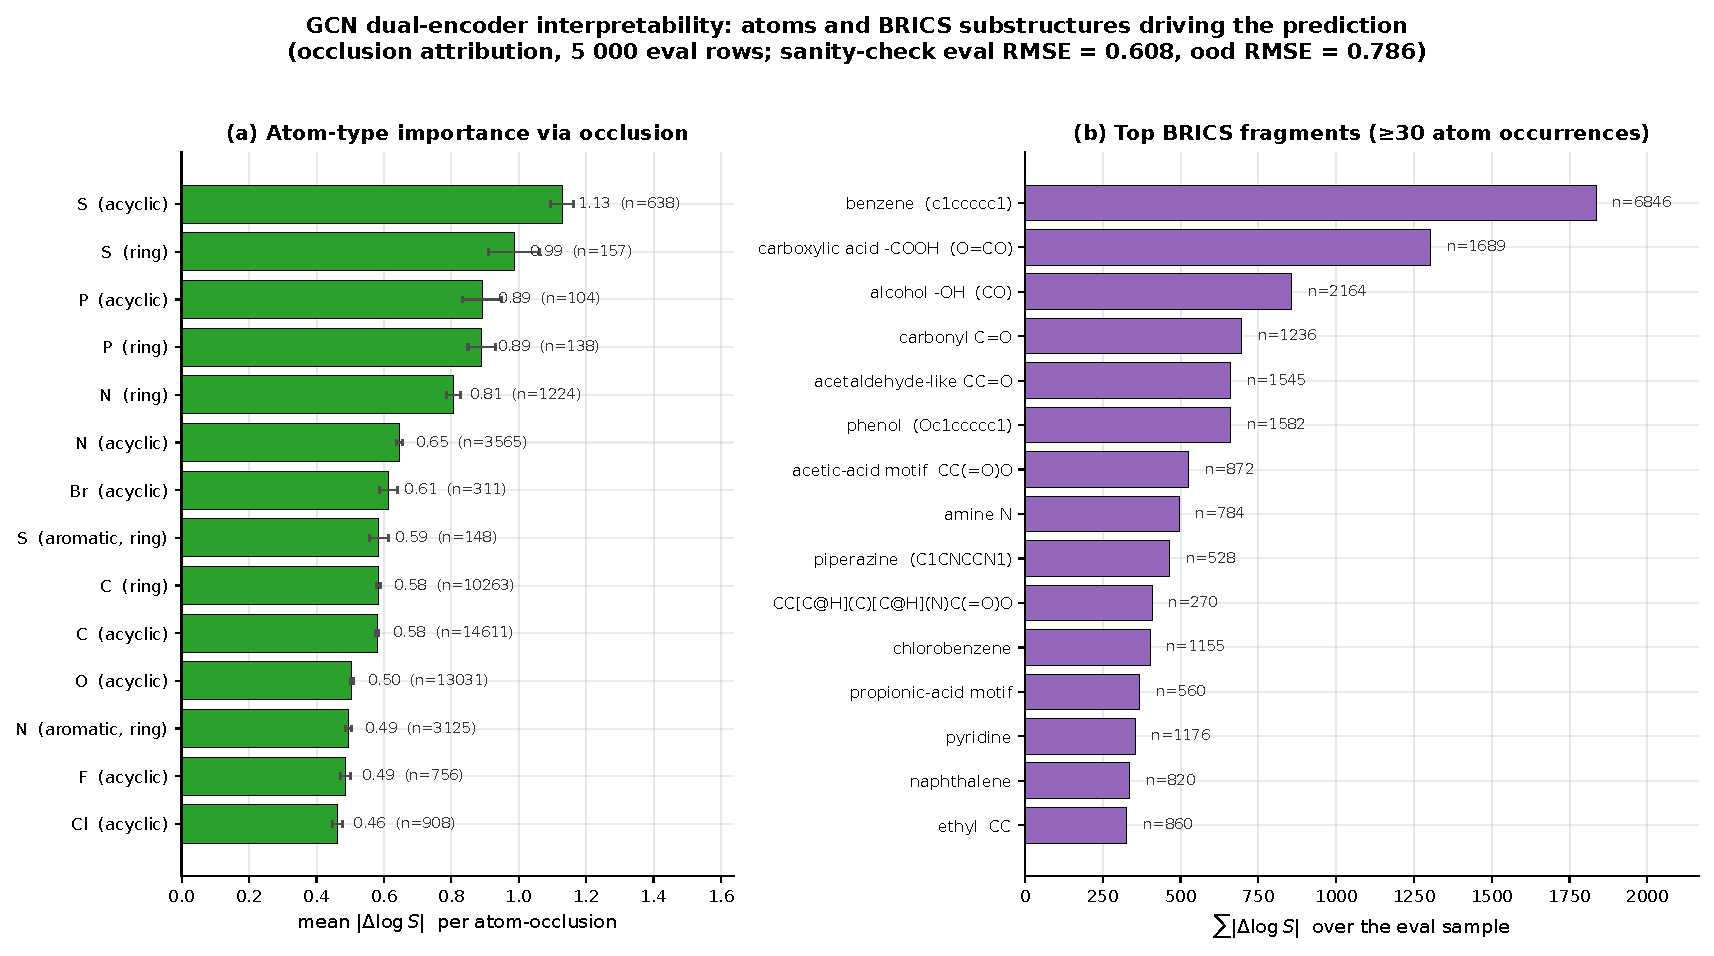
\includegraphics[width=\linewidth]{figures/fig7_gcn.pdf}
\caption{\textbf{GCN dual-encoder interpretability.}  (a) Mean
\(|\Delta\,\logS|\) per atom-occlusion, broken down by RDKit atom
``kind'' (element \(\times\) aromaticity \(\times\) ring membership)
on the eval-split sample; error bars are \(\sigma/\sqrt{n}\).  Heavy
heteroatoms (S, P, N) dominate; aromatic carbon and aliphatic
ring-carbon are essentially equivalent.  (b) Total
\(\sum |\Delta\,\logS|\) per BRICS substructure, for fragments that
appear at least 30 times in the sample.  Every top fragment is a
chemistry-textbook solubility motif; no opaque substructure makes
the top 15.}
\label{fig:interp_gcn}
\end{figure}

The atom-type ranking is led by sulfur and phosphorus: occluding a
single acyclic sulfur atom shifts the prediction by
\(\approx\) \numval{1.13} \logS{} on average -- about twice the effect
of a typical carbon (\numval{0.58}).  Sulfur and phosphorus appear
relatively rarely in the dataset (\numval{638} acyclic-S and
\numval{104} acyclic-P out of \(\sim\)\,\numval{85000} atom
occurrences) but each occurrence carries large weight, which matches
the chemical intuition that sulfones, thiols, sulfonates,
phosphonates, etc. dramatically change solubility.  Aromatic carbon
and aliphatic ring-carbon have nearly identical mean \(|\Delta|\)
\(\approx\) \numval{0.58}, consistent with the GCN being built on
seven plain atom features without an explicit \(\pi\)-system
descriptor: aromaticity is encoded only as a topology cue.

The BRICS fragment ranking is the chemically actionable view.  Every
fragment in the top fifteen is one a medicinal chemist would
immediately list as a solubility-relevant motif: aromatic core
(benzene, phenol, naphthalene, chlorobenzene, pyridine,
nitrobenzene), H-bonding groups (carboxylic acid, amide-like,
phenolic OH), small carbonyls, an alcohol motif, and amine or
piperazine ring.  No uninterpretable fragment appears in the top
twenty, which is a strong indication that the GCN is using
message-passing to aggregate chemistry-meaningful subgraphs even
though it was never explicitly told what they are.

The aggregate tables make the result statistically stable, but they
hide what a graph explanation looks like on a single molecule.  We
therefore draw four representative solutes in
Figure~\ref{fig:interp_gcn_examples}.  For each molecule we run the
same occlusion experiment atom-by-atom, but keep the sign:
\(\Delta_i = f(G) - f(G \setminus i)\), where \(G\setminus i\)
means zeroing atom \(i\)'s node features while leaving the topology
intact.  Red halos mark atoms that raise the predicted \logS{}; blue
halos mark atoms that lower it.  This produces the same kind of
visual field as a graph attention map, but it is tied directly to a
measured change in the model output.

\begin{figure}[t]
\centering
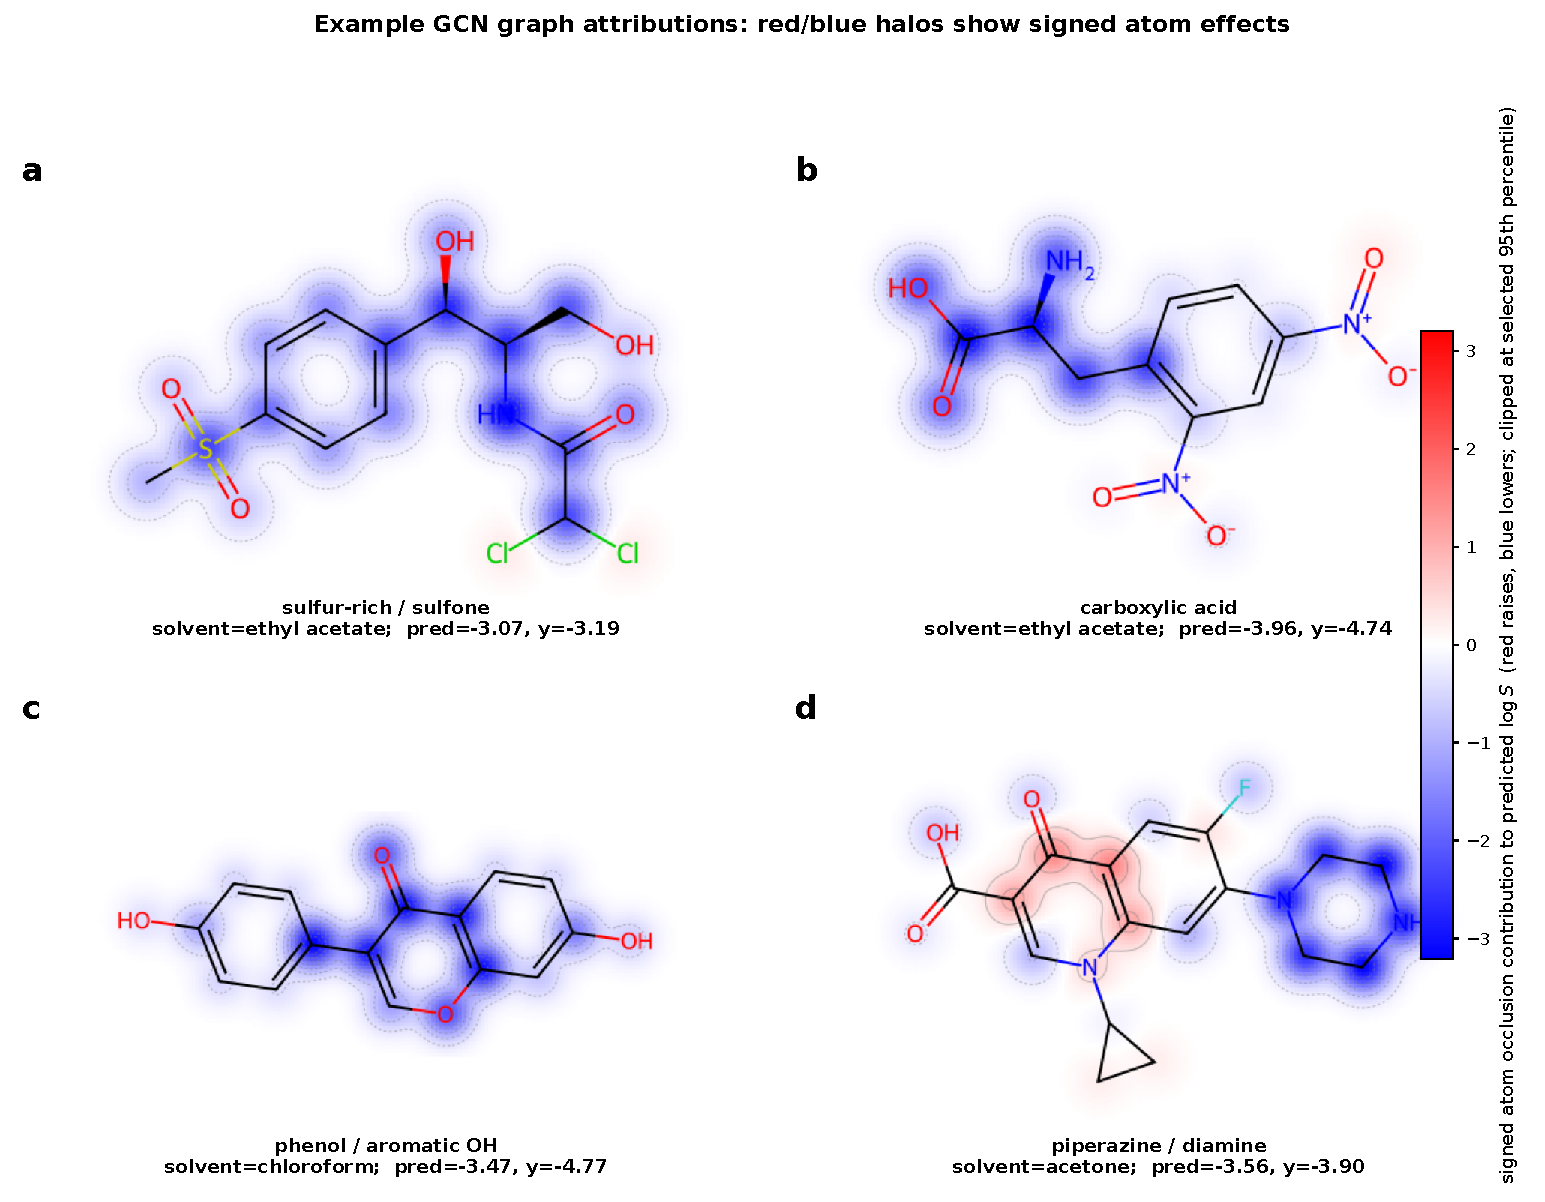
\includegraphics[width=\linewidth]{figures/fig9_gcn_molecule_examples.pdf}
\caption{\textbf{Example GCN graph attributions.}  Four solutes were
chosen from the \texttt{eval} split to expose the motifs that dominate
the aggregate BRICS ranking: sulfur/sulfone, carboxylic acid /
nitro-aromatic, phenol/aromatic OH, and piperazine/diamine.  The
underlying attribution is signed atom occlusion: red regions increase
the predicted \logS{} relative to the same graph with that atom's
features zeroed; blue regions decrease it.  The maps are qualitative
but coherent: acidic, nitro, sulfone, and amide-like atoms are
high-leverage; aromatic scaffolds often provide broad negative fields;
and heteroatom-rich fragments such as piperazine or carboxylate
dominate local prediction changes.}
\label{fig:interp_gcn_examples}
\end{figure}

These molecule-level maps also clarify what the aggregate BRICS plot
cannot.  The same functional group can participate in different
directions depending on its scaffold and solvent: a carboxylate can
be blue in a nitroaromatic acid because it lowers the prediction
relative to the rest of that molecule, while the same carboxylate
fragment still appears globally important in Figure~\ref{fig:interp_gcn}
because its occlusion magnitude is large.  This is why we report both
views: signed maps are mechanistic examples; aggregate BRICS counts
are the stable population-level result.

% -----------------------------------------------------------------------------
\subsection{What the interpretability says}
\label{sec:interp_summary}

The seven analyses above converge on a coherent story.

\begin{enumerate}
  \item \textbf{The model has independently rediscovered the General
        Solubility Equation.}  Across all three descriptor
        representations the top global features are TPSA, BertzCT,
        MolLogP, a solvent polarity proxy, and temperature -- the GSE
        axes -- without any chemistry prior.
  \item \textbf{Signed SHAP gives the chemically directional story.}
        High temperature raises predicted solubility, while high
        solute polarity/complexity features (TPSA, BertzCT, Abraham
        \(E/S/B/A\)) lower the global multi-solvent prediction.  This
        is a model-conditional aggregate statement, not a universal
        aqueous-solubility rule, and motivates the per-solvent slices.
  \item \textbf{Abraham/LSER cross-terms emerge in the SHAP interaction
        values.}  On Abraham-only the top eight interactions are
        within-LSER ($E\!\times\!V$, $S\!\times\!E$, etc.); the
        cross-block pairs that appear next are matched-axis
        solute-solvent terms ($E\!\times\!E$, $A\!\times\!A$,
        $E\!\times\!B$).  On RDKit the largest cross-block pair is
        $\texttt{BertzCT}\!\times\!\texttt{MaxPartialCharge}$, the
        discrete analogue of a partition-coefficient term.
  \item \textbf{Descriptor representations recover the four classical
        solvent families} (water, alkanes, polar aprotic+aromatic,
        polar protic alcohols) under SHAP-fingerprint clustering.
        Circular fingerprints fail to recover this taxonomy and group
        solvents by shared substructure bits instead -- the
        mechanistic reason the Representation ablation finds them
        \(+\)\numval{0.15} \RMSE{} worse on \texttt{ood} and
        \texttt{sc3\_gold}.
  \item \textbf{The solute drives the prediction (\(\sim\)\numval{70}\,\%
        of attribution mass), not the solvent} (\(\sim\)\numval{22}\,\%).
        Moving \texttt{eval}\,\(\to\)\,\texttt{ood} shifts \numval{3}--\numval{6}
        percentage points solute\(\to\)solvent -- the expected
        behaviour of a model that uses solvent identity as a coarse
        switch and solute identity as the regression target.
  \item \textbf{Water and n-hexane are special.}  They are the only
        two solvents in which solvent-side features take the top-2
        per-solvent ranks -- the model treats them as a gating signal
        and only then evaluates the solute.
  \item \textbf{The GCN has learned a substructure ontology that
        matches medicinal chemistry intuition.}  Every top BRICS
        fragment under occlusion attribution is a textbook
        solubility-relevant motif (benzene, carboxylic acid, phenol,
        carbonyl, pyridine, naphthalene, nitrobenzene, piperazine);
        no uninterpretable motif appears in the top 20, and the signed
        example maps show those motifs as coherent local red/blue
        attribution fields rather than isolated single atoms.
  \item \textbf{Heavy heteroatoms drive GCN attribution.}  Removing a
        single acyclic sulfur shifts the prediction by
        \(\sim\)\numval{1.13}\,\logS{}, twice the effect of removing
        a carbon -- both a sanity check (rare, polar, heavy
        heteroatoms matter) and an actionable handle for SAR-guided
        users.
\end{enumerate}

\paragraph{Caveats.}  All interpretations above are computed at
seed\,$=$\,\numval{42}.  The Representation ablation shows seed-to-seed
\RMSE{} jitter is \(\sim\)\numval{0.005}; we therefore expect the
top-3 features per featurizer to be stable across seeds, but ranks
beyond \(\sim\)\numval{10} could reshuffle.  Tree-SHAP interaction
values are computed in full only for Abraham-only (16 features,
exact); RDKit uses a smaller \numval{200}-row sample with
\texttt{tree\_limit}\,$=$\,\numval{150}, and Mordred / Morgan /
Atom-Pair / MACCS interaction values are skipped because the
$O(N \cdot T \cdot F^2)$ cost is prohibitive on a single CPU.  The
block-level interaction story is rigorous for all seven featurizers
through the block-wise main-effect decomposition of
Section~\ref{sec:interp_blockwise}.  Signed SHAP directions are
rank-correlations between feature values and SHAP values, so they
should be read as fitted-model associations, not causal derivatives.
GCN attribution uses ``soft'' node-feature occlusion (zero the node
features, keep the topology), which preserves message-passing
well-definedness; exact subgraph deletion would invalidate
cross-molecule comparison.  The molecule maps in
Figure~\ref{fig:interp_gcn_examples} are illustrative examples
selected for chemically recognisable motifs; the population-level
claim remains the BRICS/atom-type aggregation in
Figure~\ref{fig:interp_gcn}.  The OOD per-solvent analysis is computed
and released, but not surfaced in this section because OOD has 162
solvents with highly skewed counts; the dominant findings (block
shares, solvent clustering) are reported on \texttt{ood} alongside
\texttt{eval} where directly comparable.

\paragraph{Reproducibility.}  All scripts, intermediate SHAP arrays
($\sim$\numval{420}\,MB), 85 figures, and per-solvent CSV summaries
live under
\path{vansh/Ablations/Interpretability/} in the released repository.
Each driver script is resumable and runs single-seed end-to-end in
\(\sim\)\numval{15} minutes (LightGBM SHAP) or \(\sim\)\numval{30}
seconds (GCN occlusion) on the development cluster.

% \section{Discussion}
\label{sec:discussion}

\scthree{} is meant to separate what is knowable about multi-solvent solubility from what is an artifact of noisy literature aggregation.
Three limitations deserve emphasis while headline benchmark numbers are still being finalised.

\paragraph{Multi-source sparsity.}
Consensus tiers and $\sigma$ rely on $(\text{solute},\text{solvent})$ pairs that appear in multiple independence groups after copycat merging.
This subset is informative but thin relative to the full cleaned table; conclusions about $\epsA$, tier coverage, and Z-RMSE should be read as statements about \emph{that} multi-source slice, not about every measurement row.

\paragraph{Comparable training protocols.}
Some foundation-model rows remain incomplete or use provisional hyperparameters; until every method is trained with matched tuning budget and reported variance, ranking gaps involving those rows should be interpreted cautiously.

\paragraph{Numerical harmonisation.}
Several distinct quantities appear throughout the manuscript---global inter-group $\epsA$, duplicate-triple floors $\epsA^{(s)}$ per split (§\ref{sec:data_scaling}), and consensus $\sigma$ on tiers---each answering a different measurement question.
Before submission, all headline figures should be checked for internal consistency (single definitional paragraph in §\ref{sec:aleatoric} and §\ref{sec:data_scaling}).

Despite these caveats, the benchmark already enables analyses---scaling, transfer from quantum solvation data, feature attribution---that require calibrated uncertainty rather than point estimates alone.


% ─── References ─────────────────────────────────────────────────────────────
\bibliographystyle{plainnat}
\bibliography{references}

\end{document}
